


%%%%%%%%%%%%%%%%%%%%%%%%%%%%%%%%%%%%%%%%%%%%%%%%%%%%%%%%%%%
%%%%%%%%%%%%% RESULTADOS DE VERDAD %%%%%%%%%%%%%%%%
%%%%%%%%%%%%%%%%%%%%%%%%%%%%%%%%%%%%%%%%%%%%%%%%%%%%%%%%%%%

\begin{landscape}

\subsection{Visualización del Modelo ajustado para Mujeres y hombres}
\begin{figure}[H]
    \centering
    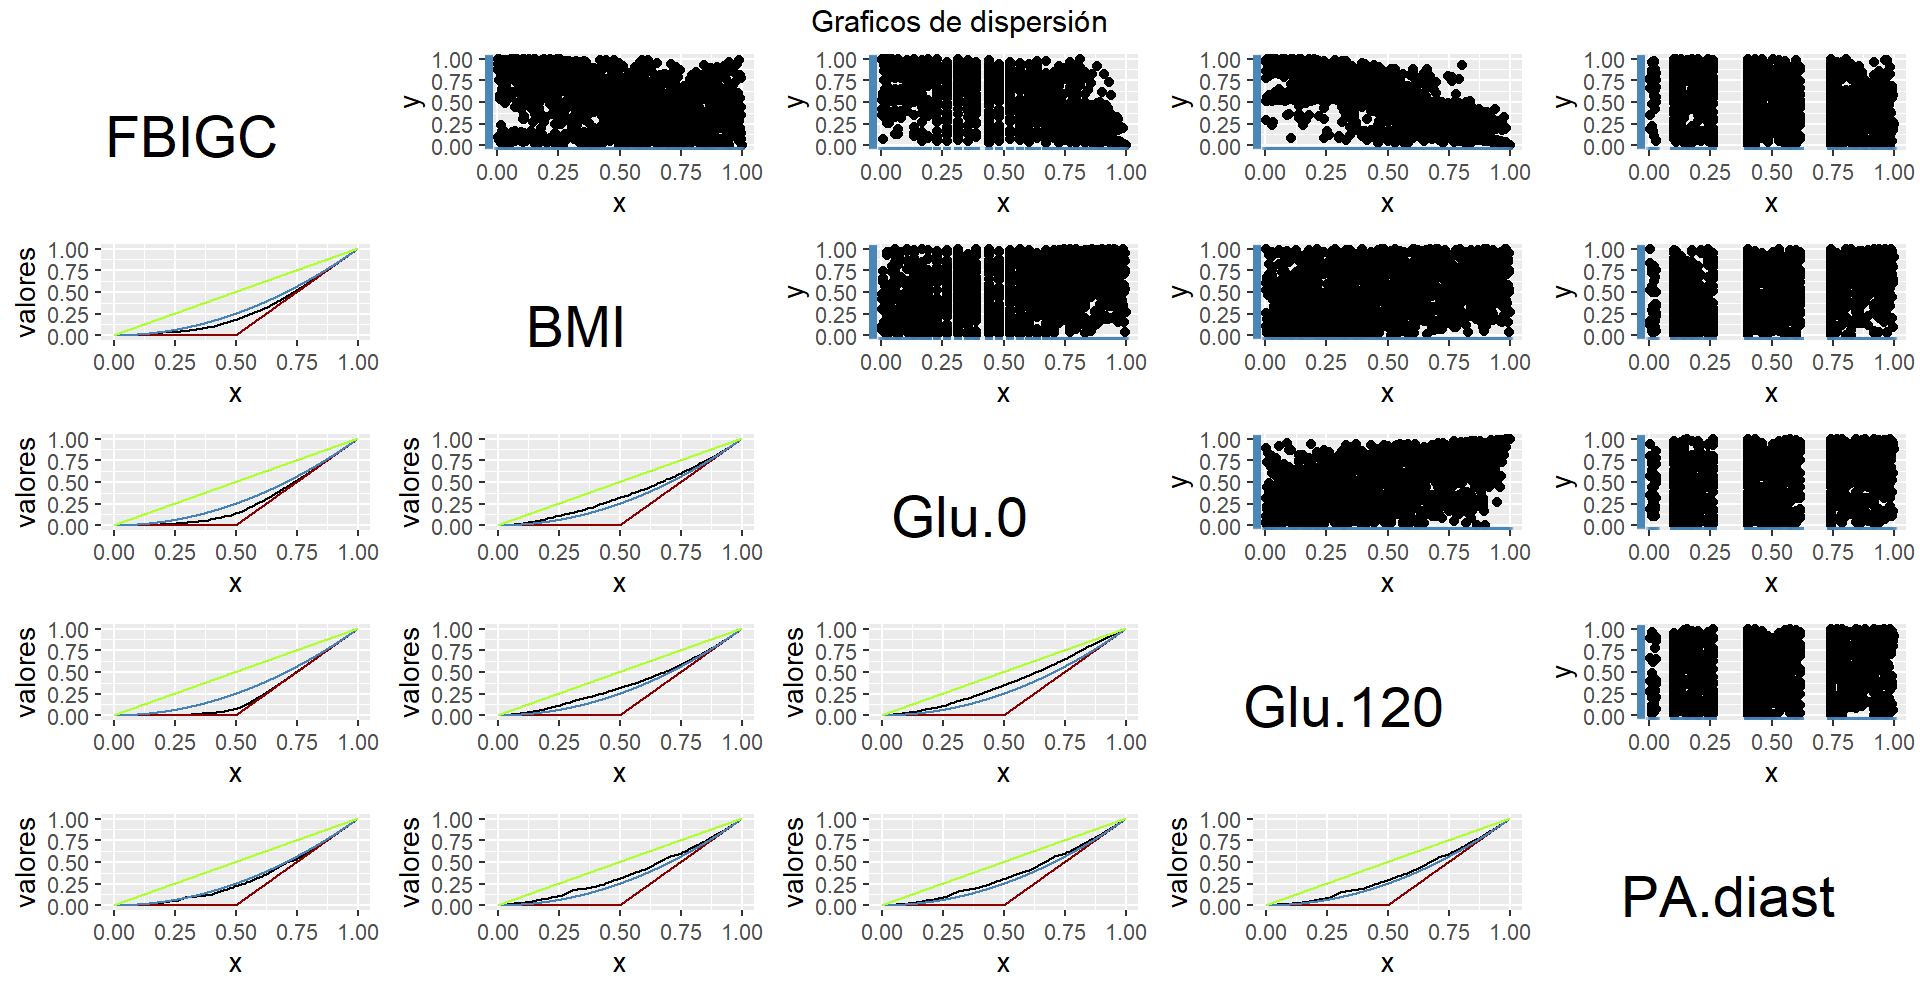
\includegraphics[height = 13.5 cm, width = 1.4 \textwidth]{4img/UdiagT.png}
    \caption{Diagonales y gráficos de dispersión en escala $u$ de hombres y mujeres.}
    \label{fig:diagTot}
\end{figure}

\end{landscape}

Uno de los aspectos más destacados de la Figura \ref{fig:diagTot}, es la posición de la diagonal de la cópula empírica en relación con la diagonal de cópula producto. En su mayor parte, la diagonal de la cópula empírica se sitúa por debajo o por encima de la diagonal, lo que indica que las dependencias entre las variables son mayoritariamente concordantes negativas o positivas, respectivamente. Este patrón de comportamiento es crucial, ya que las cópulas paramétricas pueden modelar estas relaciones de manera efectiva. Por lo tanto, como ya se había mencionado antes utilizar un modelo \texttt{R} vine con un ajuste paramétrico parece ser una estrategia apropiada.

Otro aspecto destacable es la partición que genera la variable presión diastólica. Recuérdese que esta es la presión arterial mínima registrada en las arterias durante el ciclo cardíaco cuando el corazón se encuentra en reposo entre latidos. La creación de estos tres grupos podría deberse a la presencia de tres subpoblaciones, como personas con presión diastólica normal, con hipertensión leve y con hipertensión moderada o grave o también podría provenir de las características de los instrumentos de medición. Sin embargo, no parece haber una dependencia estable con las otras variables.


Ahora, se muestran los heatmaps $\mathscr{H}\rho$, $\mathscr{H}\sigma$ y $\mathscr{H}$ de todas las cópulas utilizadas en el modelo D-vine para el modelo considerando hombre y mujeres. 


\begin{figure}[H]
 \centering
  \subfloat[$\mathscr{H}\rho_{C_{12}}$]{
   \label{C12rhoT}
    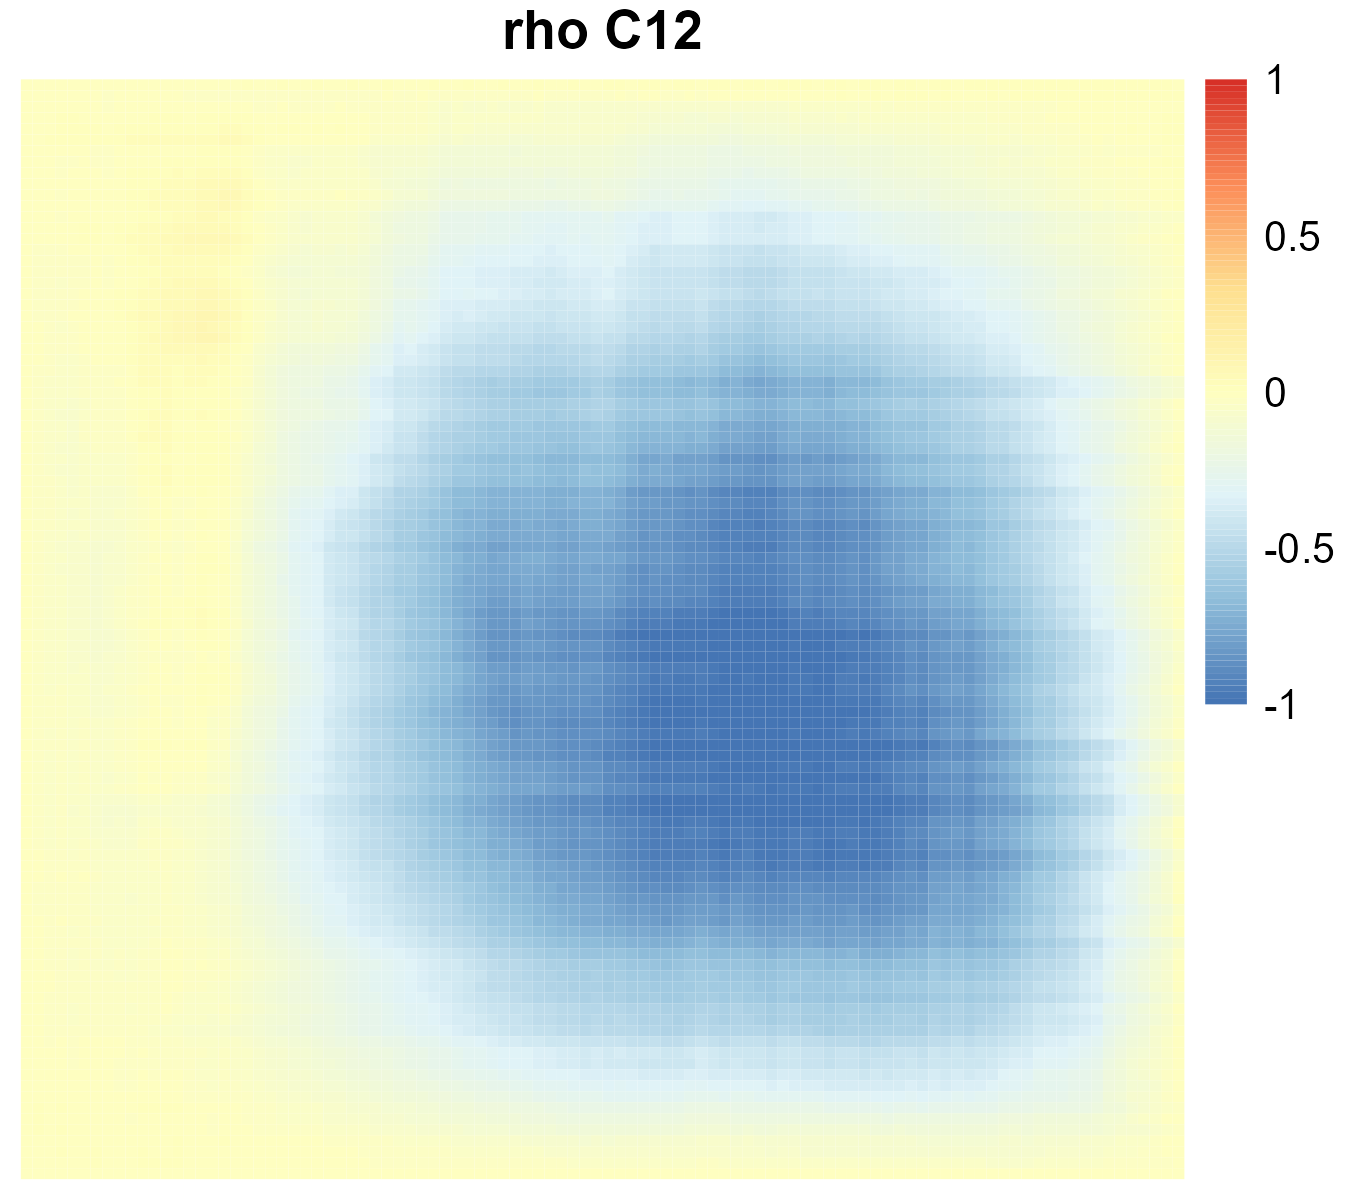
\includegraphics[width=0.3\textwidth]{4img/TotalrhoC12.png}}
  \subfloat[$\mathscr{H}\sigma_{C_{12}}$]{
   \label{C12sigmaT}
    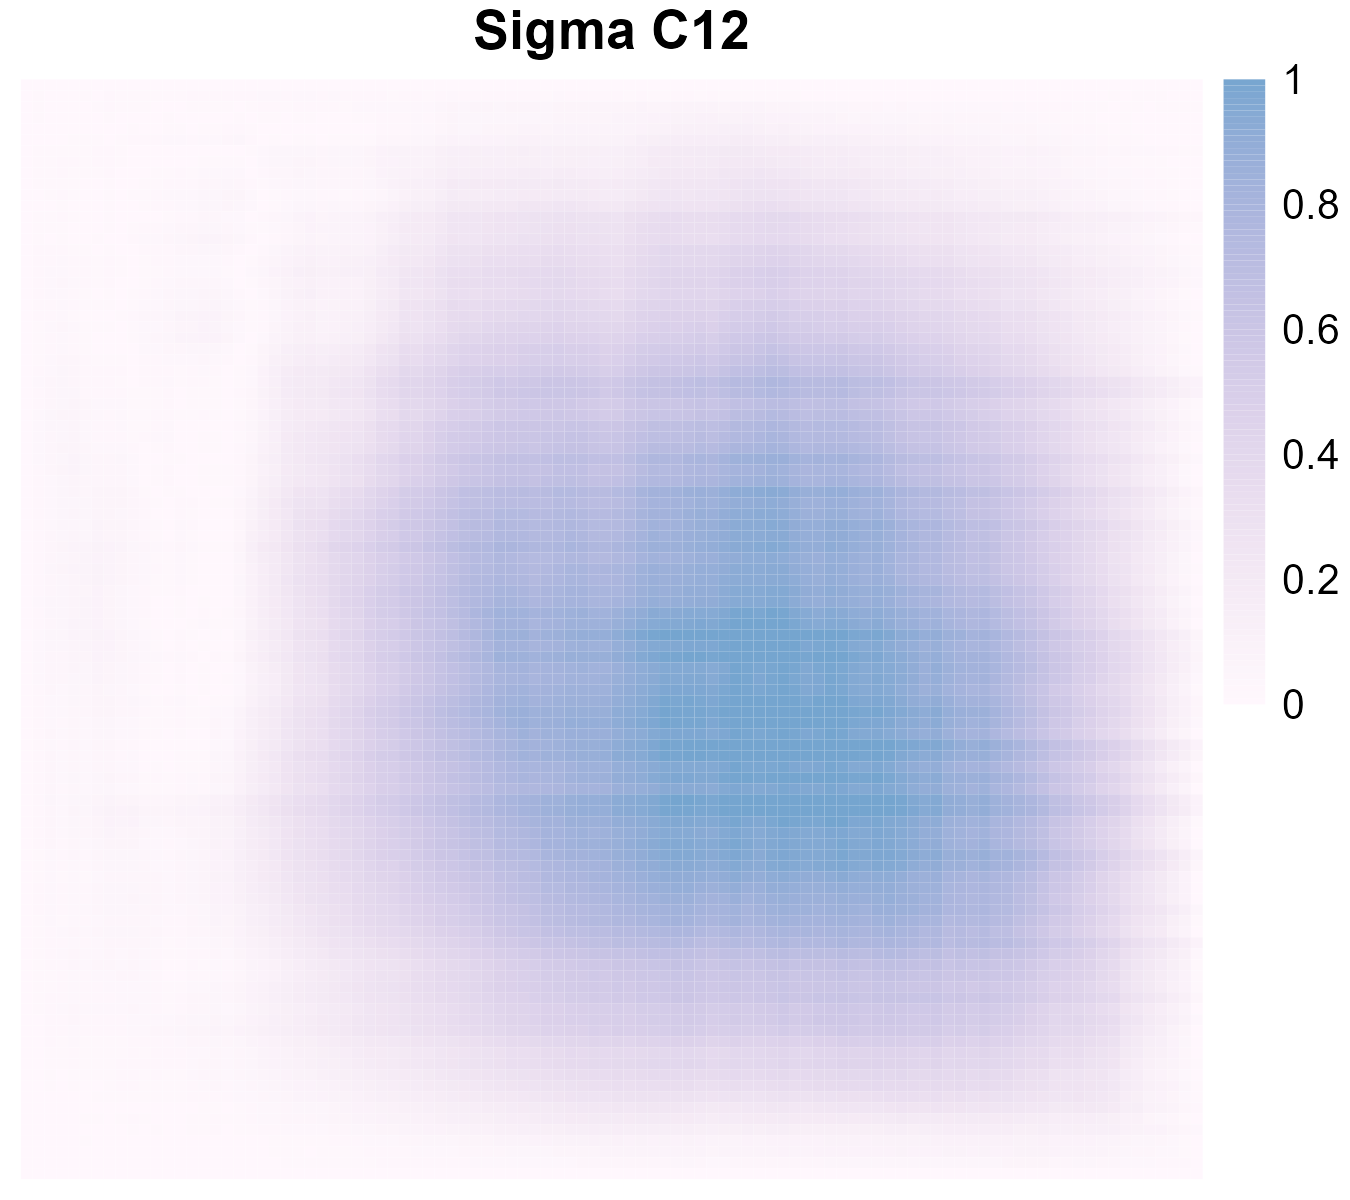
\includegraphics[width=0.3\textwidth]{4img/TotalsigmaC12.png}}
  \subfloat[$\mathscr{H}_{C_{12}}$]{
   \label{C12HT}
    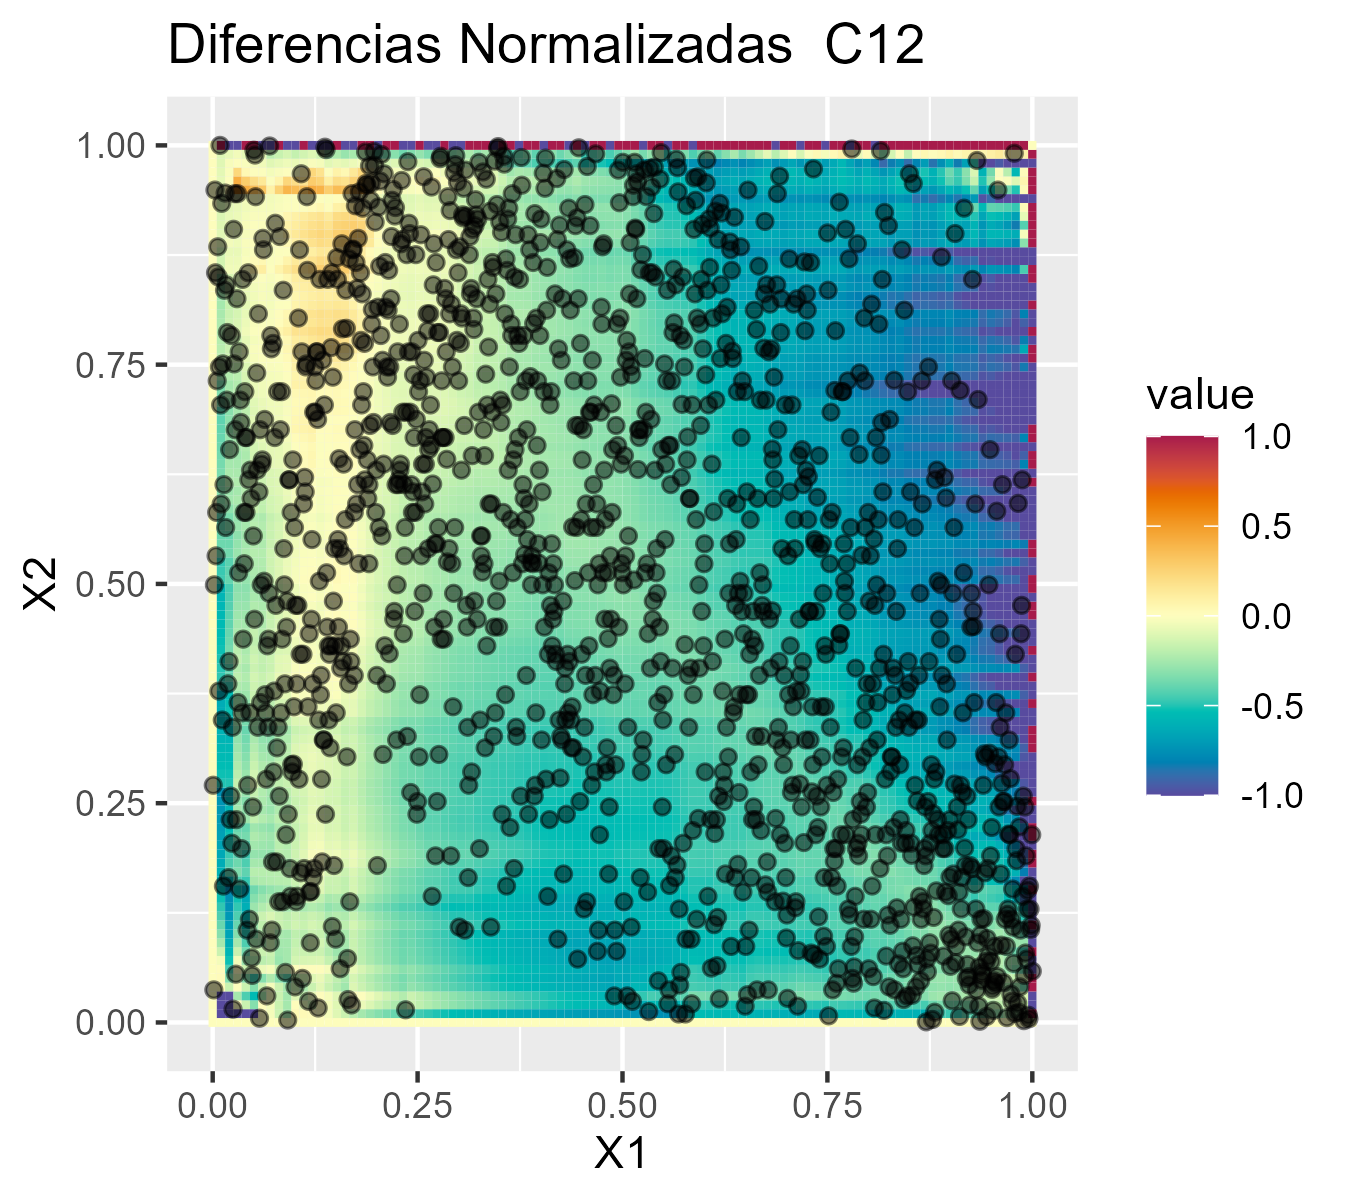
\includegraphics[width=0.3\textwidth]{4img/TotalHC12.png}}
\end{figure}

\begin{figure}[H]
 \centering
  \subfloat[$\mathscr{H}\rho_{C_{23}}$]{
   \label{C23rhoT}
    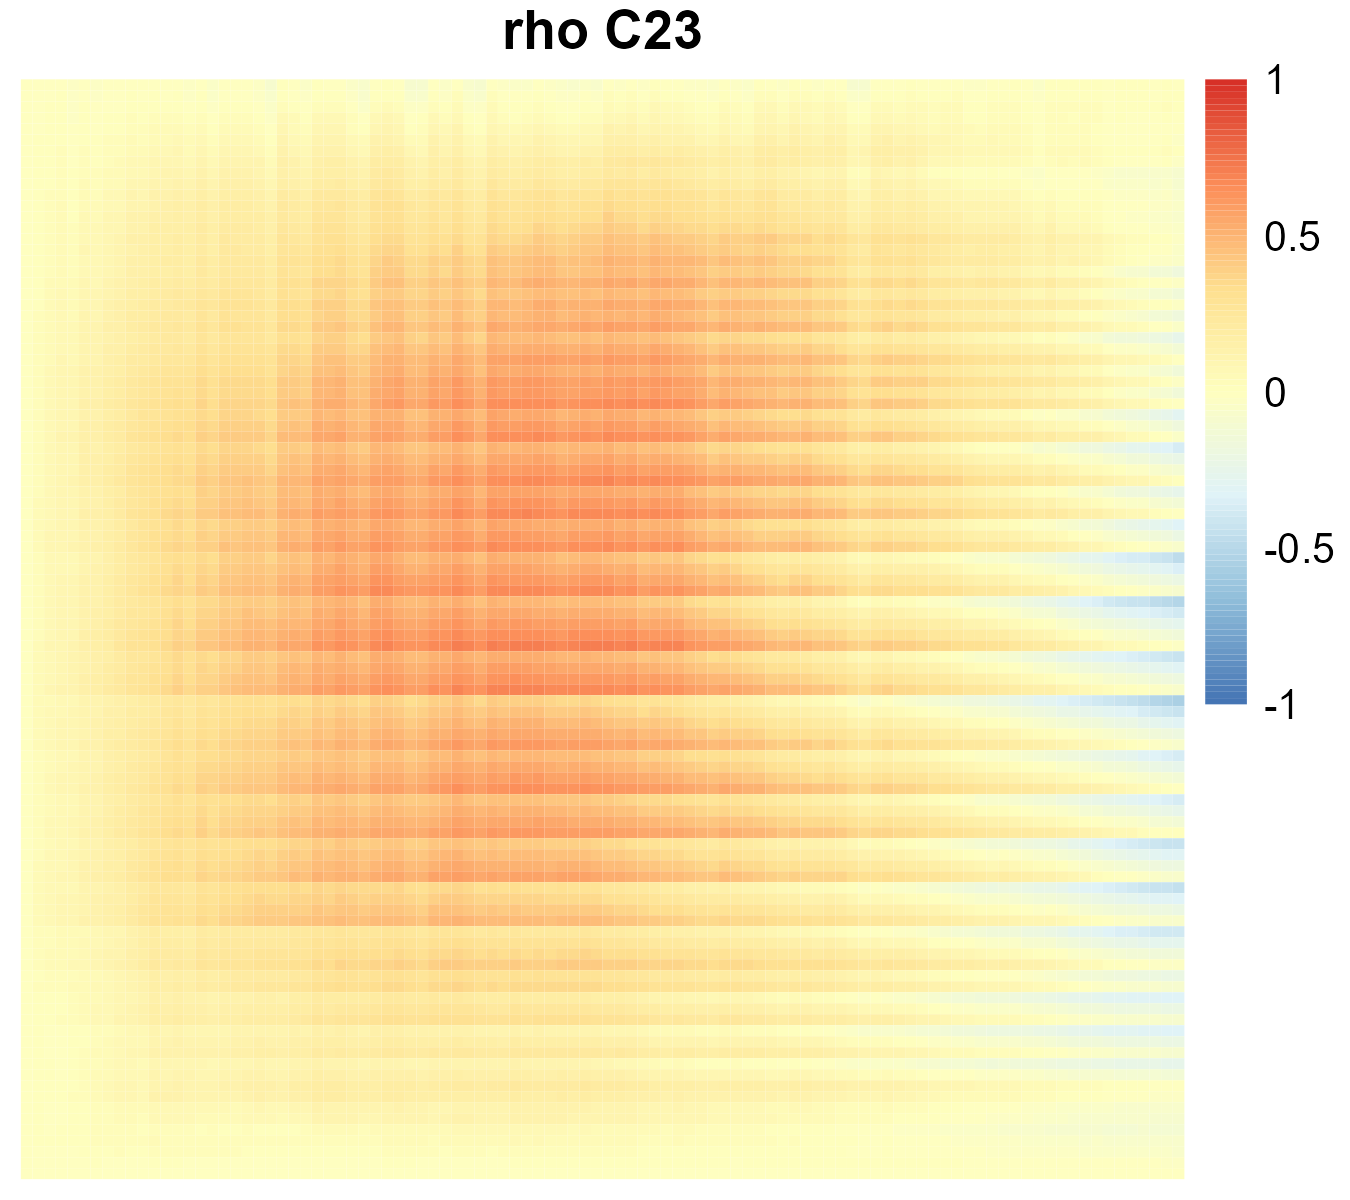
\includegraphics[width=0.3\textwidth]{4img/TotalrhoC23.png}}
  \subfloat[$\mathscr{H}\sigma_{C_{23}}$]{
   \label{C23sigmaT}
    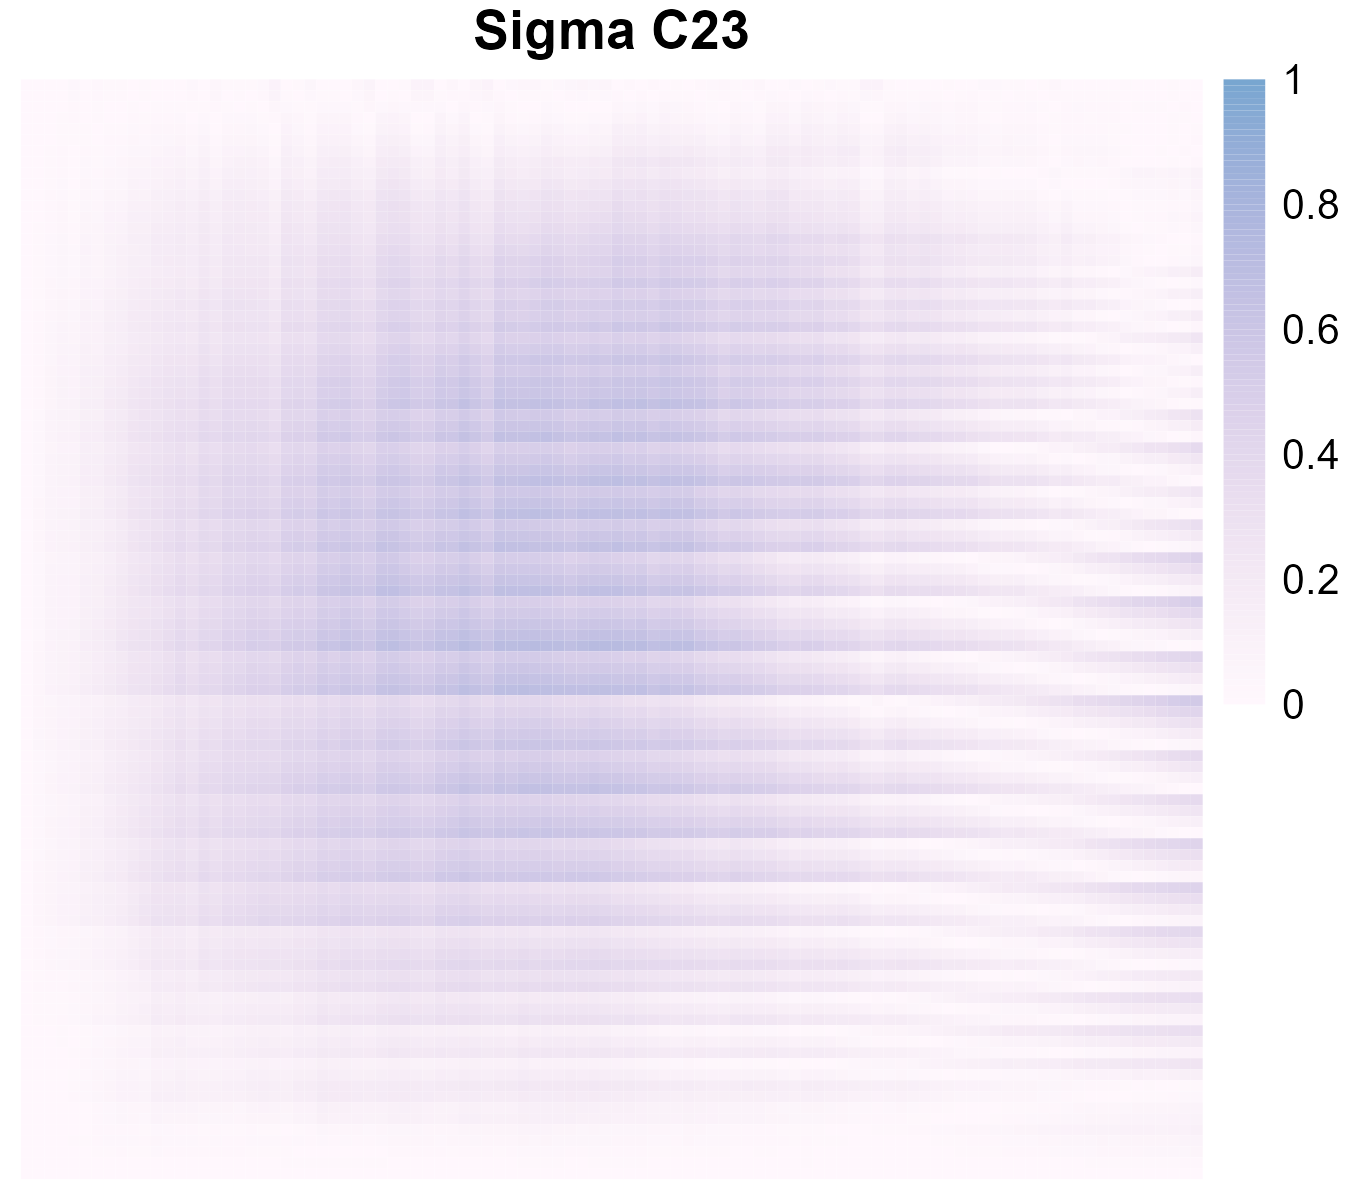
\includegraphics[width=0.3\textwidth]{4img/TotalsigmaC23.png}}
  \subfloat[$\mathscr{H}_{C_{23}}$]{
   \label{C23HT}
    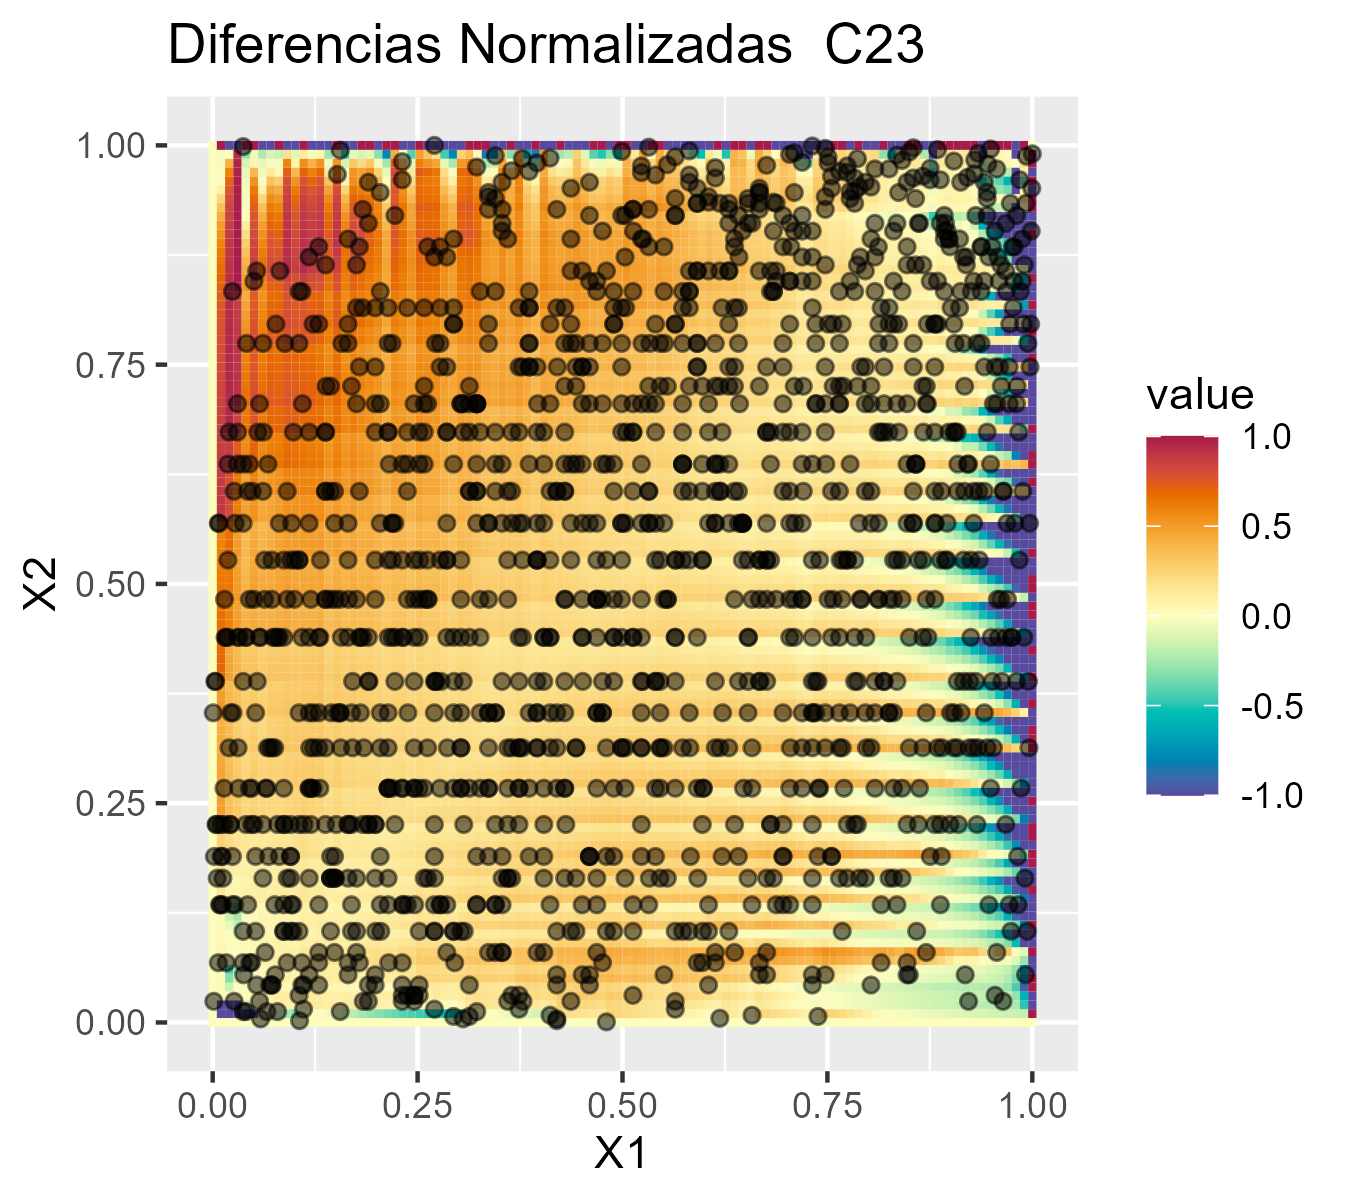
\includegraphics[width=0.3\textwidth]{4img/TotalHC23.png}}
\end{figure}

\begin{figure}[H]
 \centering
  \subfloat[$\mathscr{H}\rho_{C_{34}}$]{
   \label{C34rhoT}
    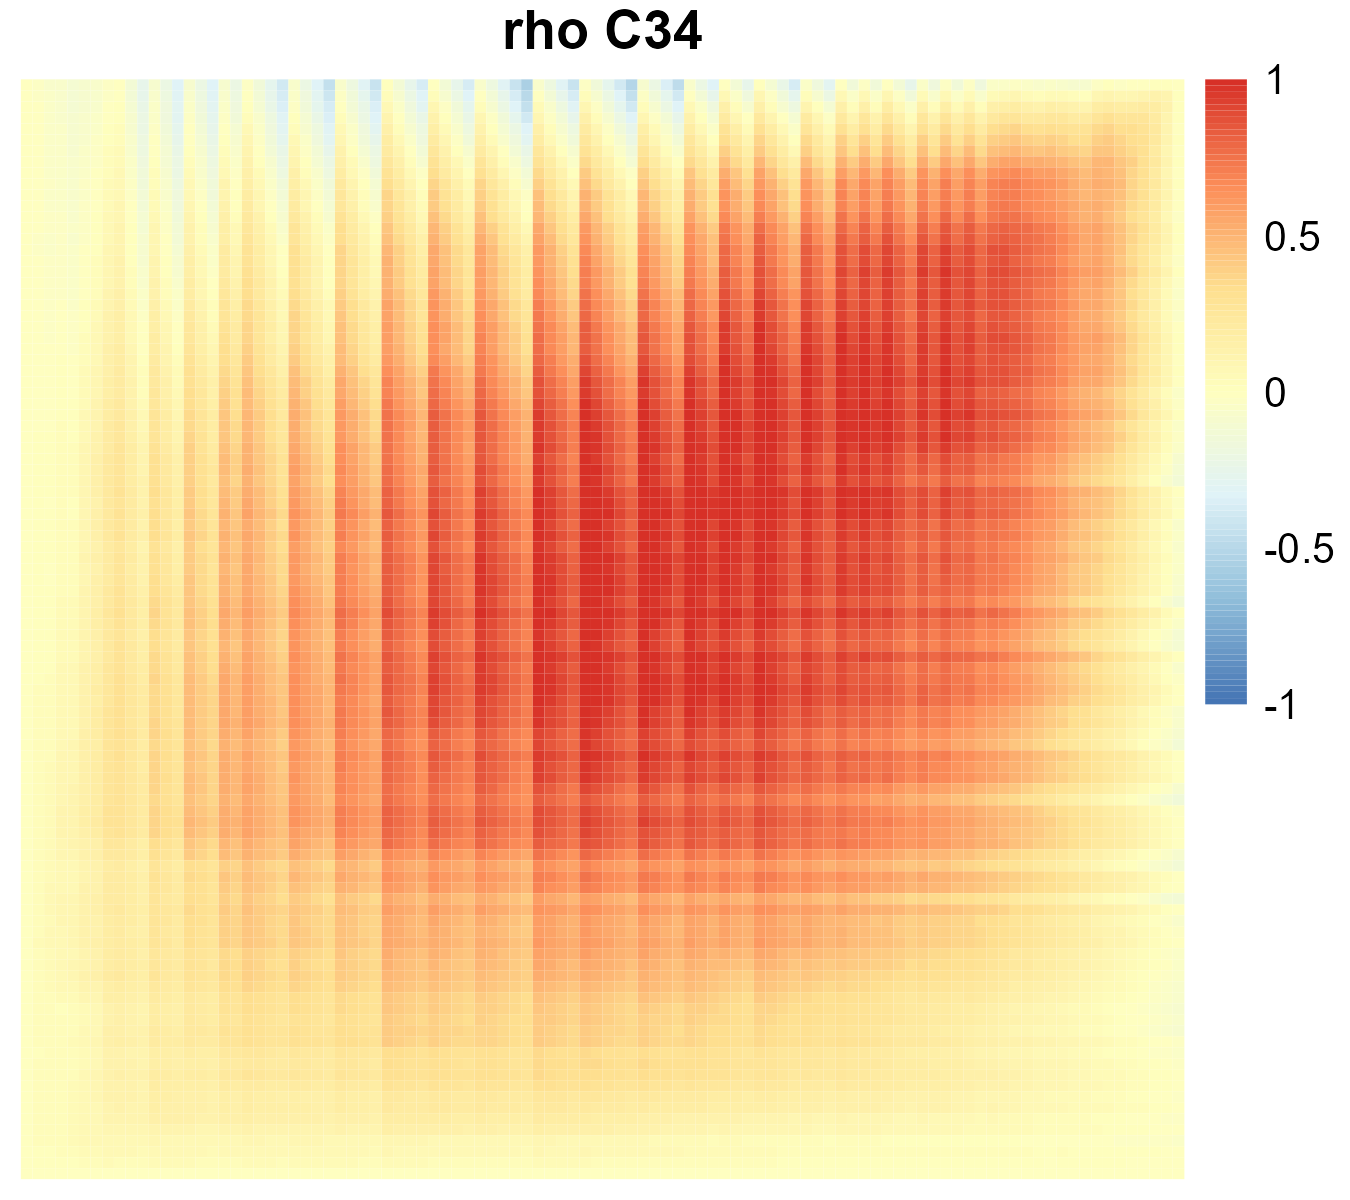
\includegraphics[width=0.3\textwidth]{4img/TotalrhoC34.png}}
  \subfloat[$\mathscr{H}\sigma_{C_{34}}$]{
   \label{C34sigmaT}
    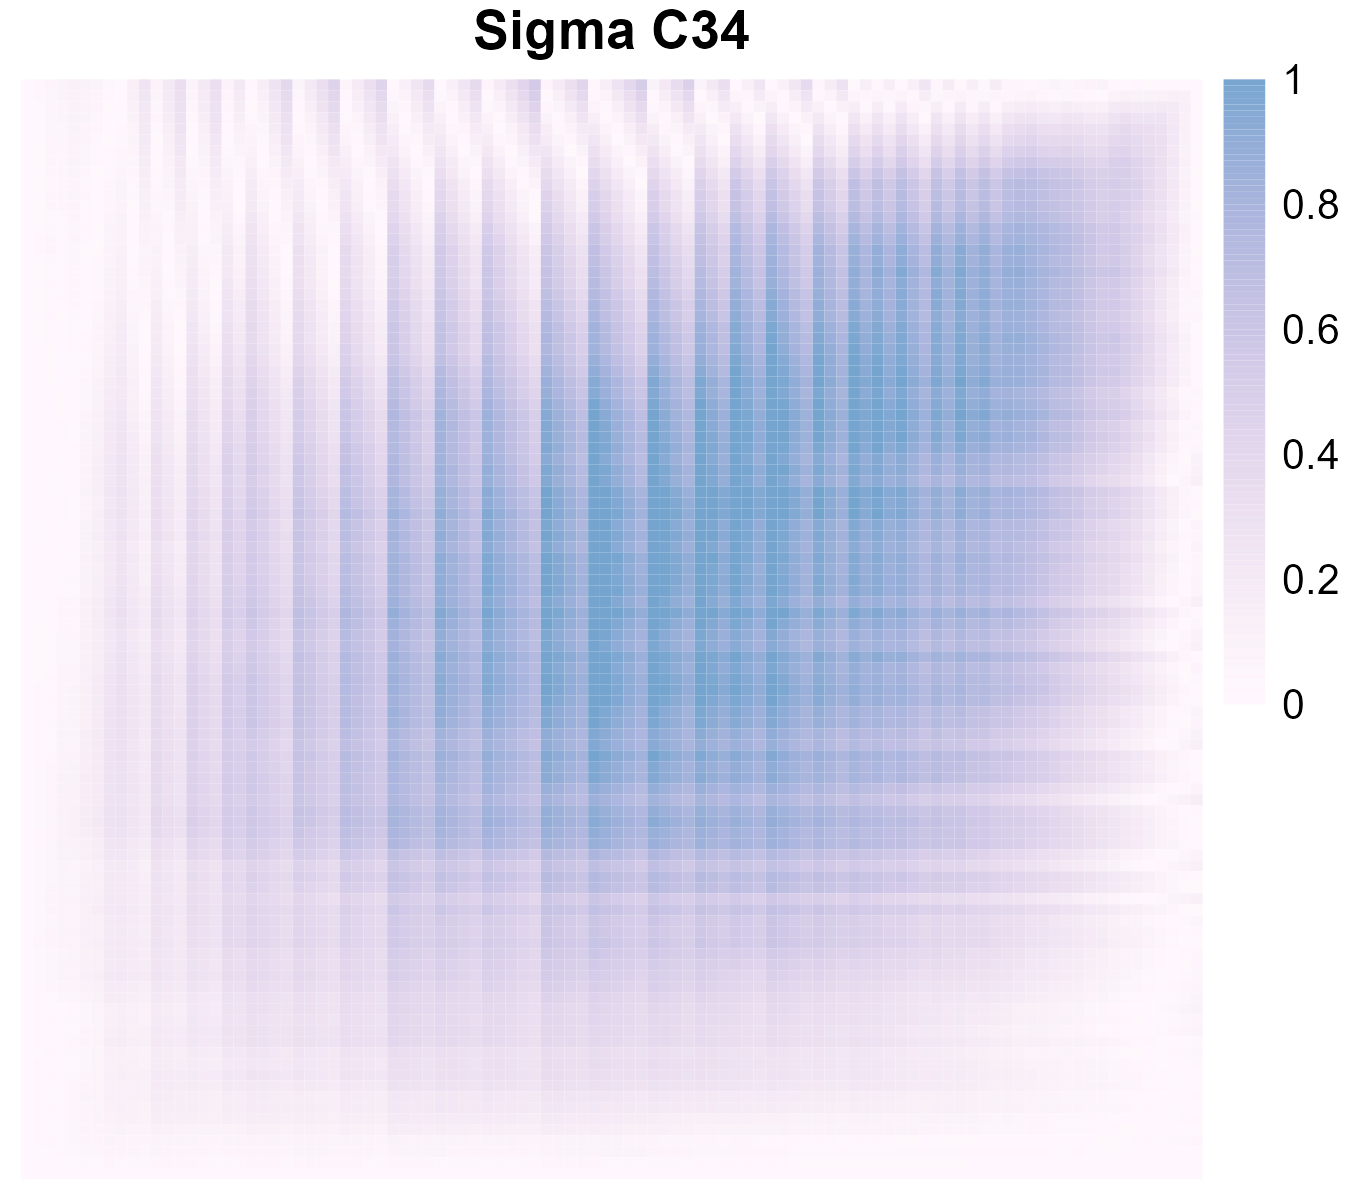
\includegraphics[width=0.3\textwidth]{4img/TotalsigmaC34.png}}
  \subfloat[$\mathscr{H}_{C_{34}}$]{
   \label{C34HT}
    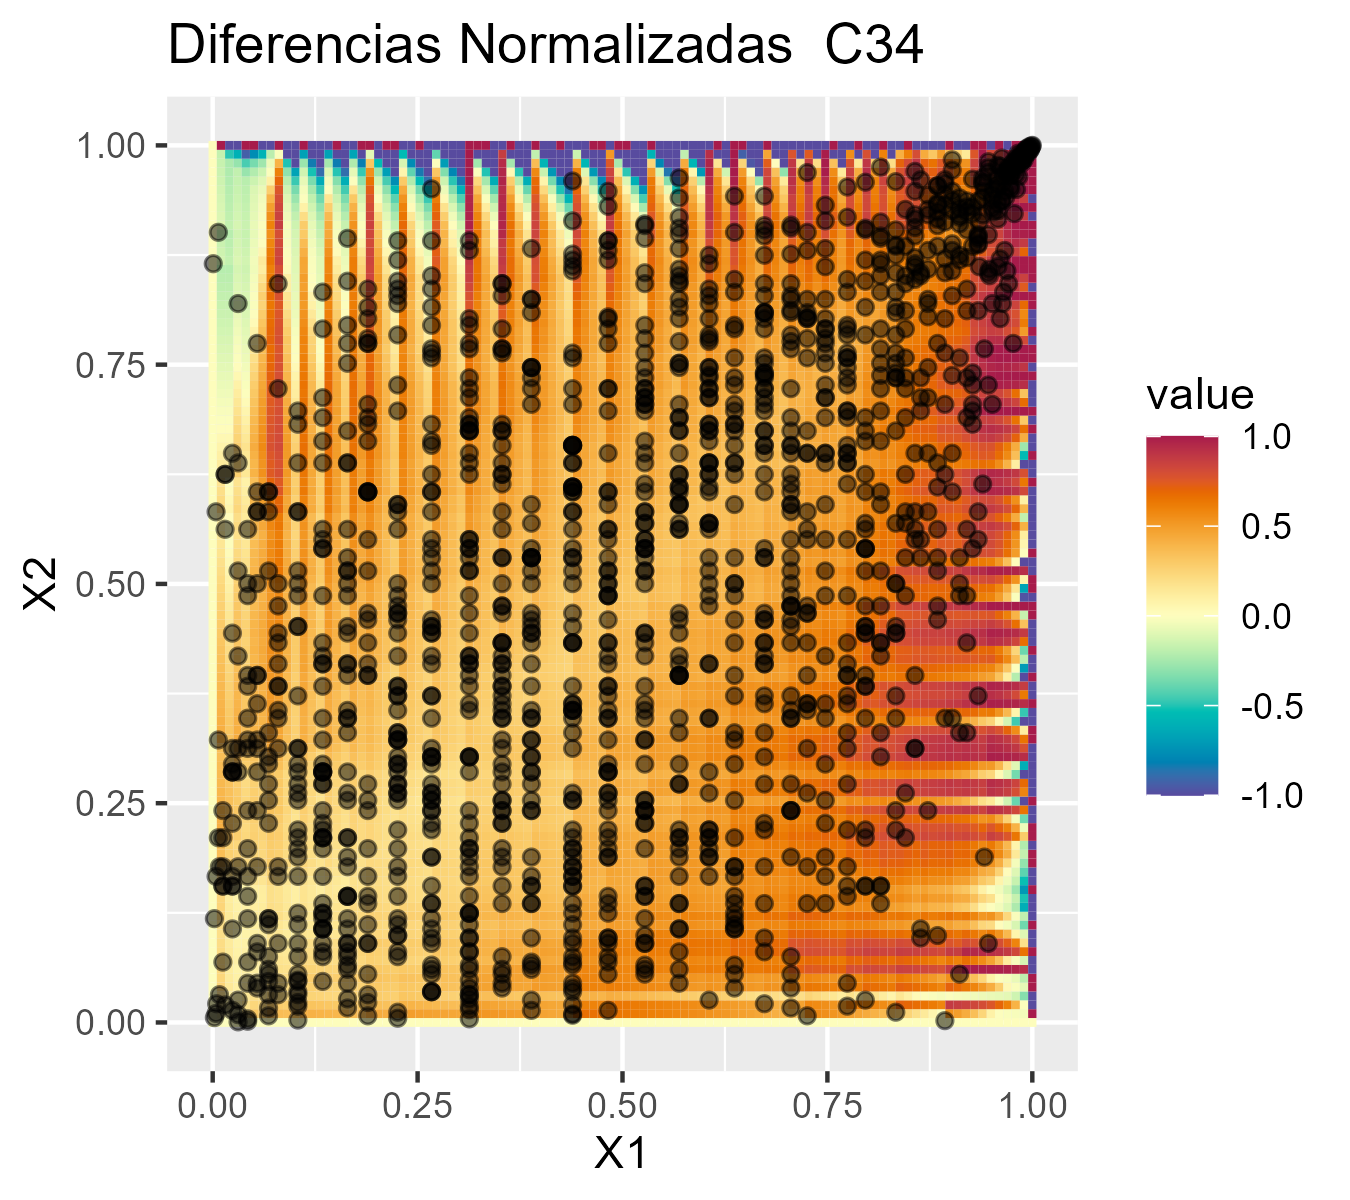
\includegraphics[width=0.3\textwidth]{4img/TotalHC34.png}}
\end{figure}

\begin{figure}[H]
 \centering
  \subfloat[$\mathscr{H}\rho_{C_{45}}$]{
   \label{C45rhoT}
    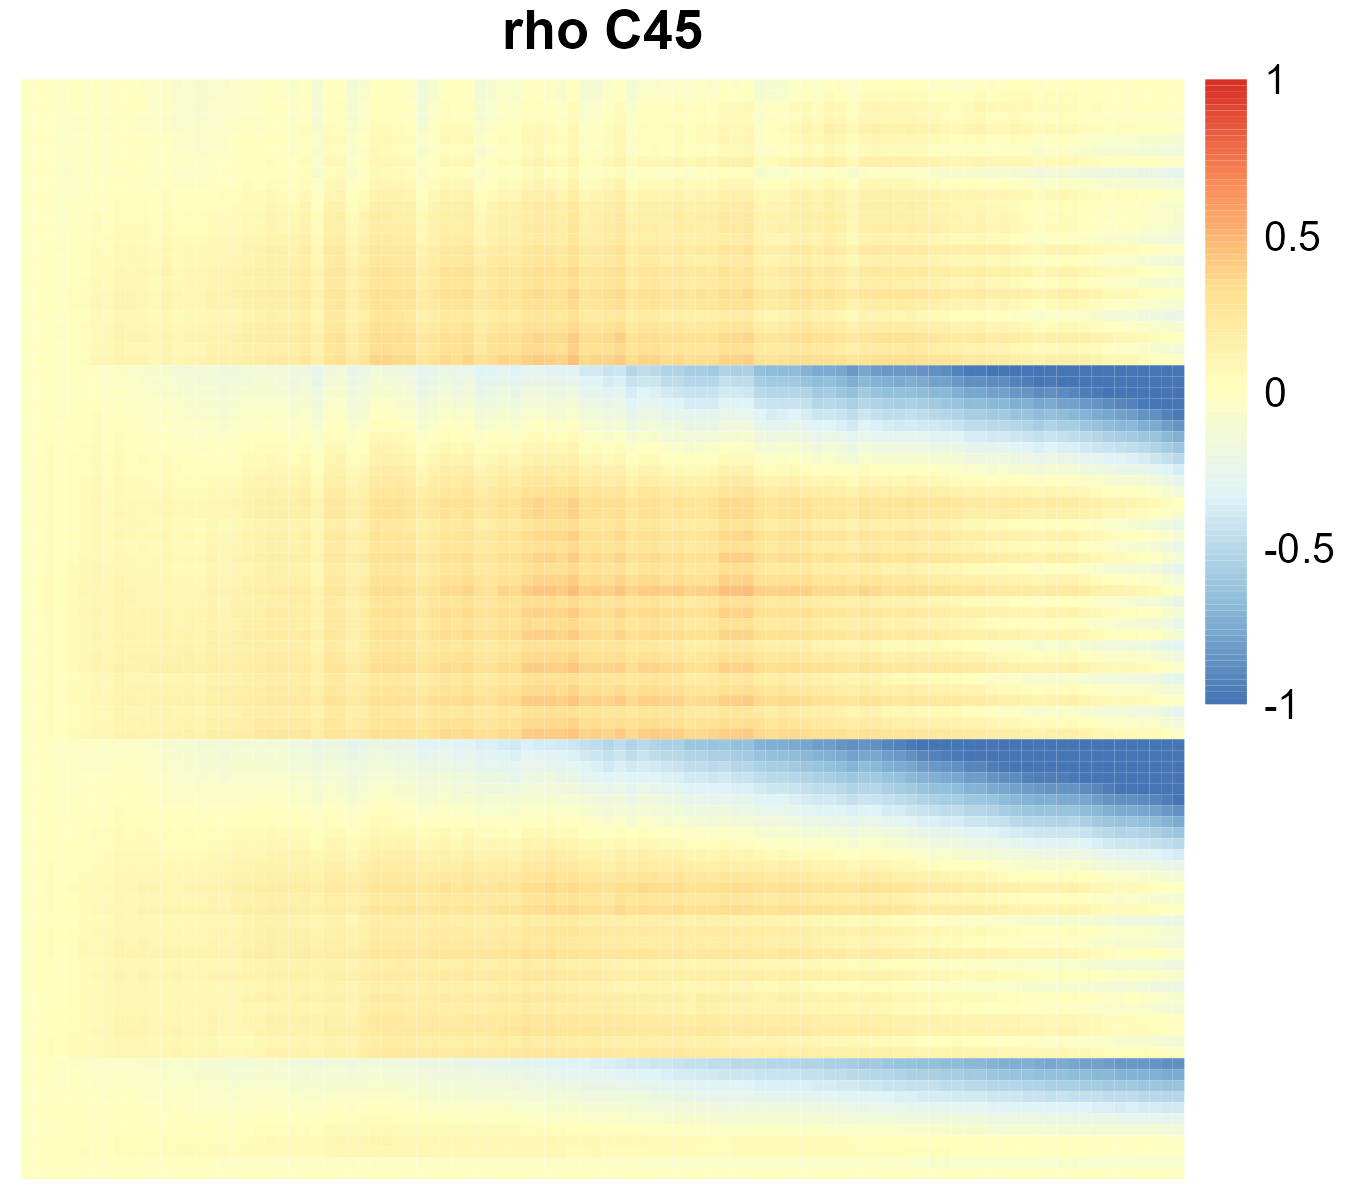
\includegraphics[width=0.3\textwidth]{4img/TotalrhoC45.png}}
  \subfloat[$\mathscr{H}\sigma_{C_{45}}$]{
   \label{C45sigmaT}
    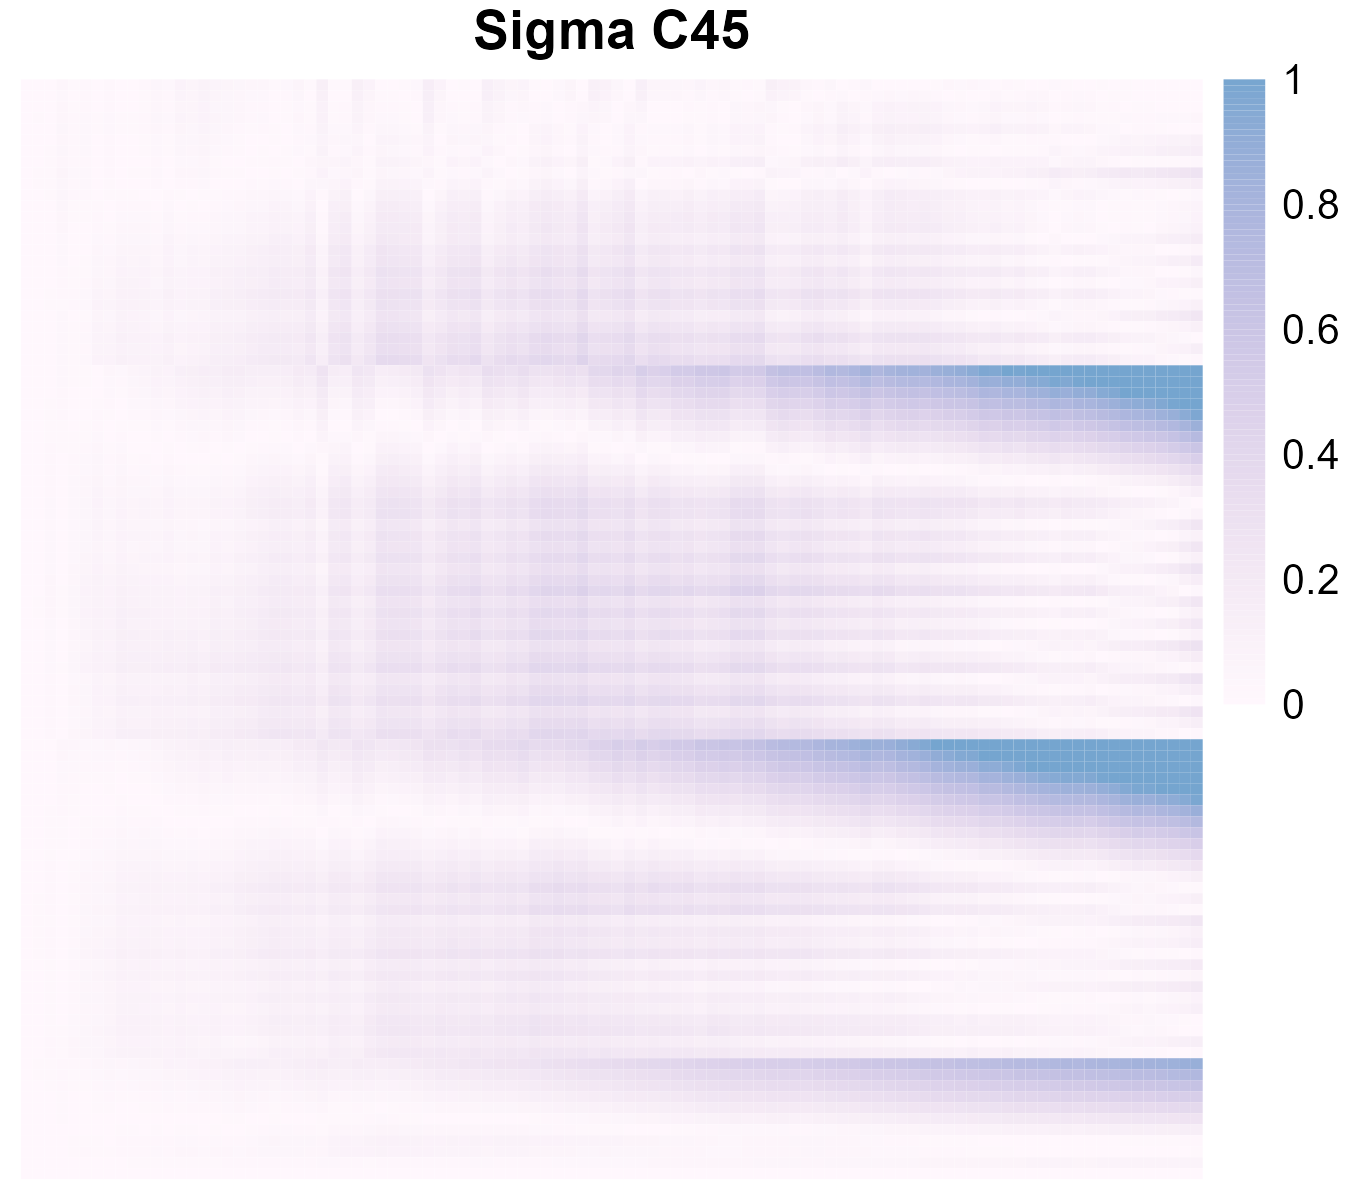
\includegraphics[width=0.3\textwidth]{4img/TotalsigmaC45.png}}
  \subfloat[$\mathscr{H}_{C_{45}}$]{
   \label{C45HT}
    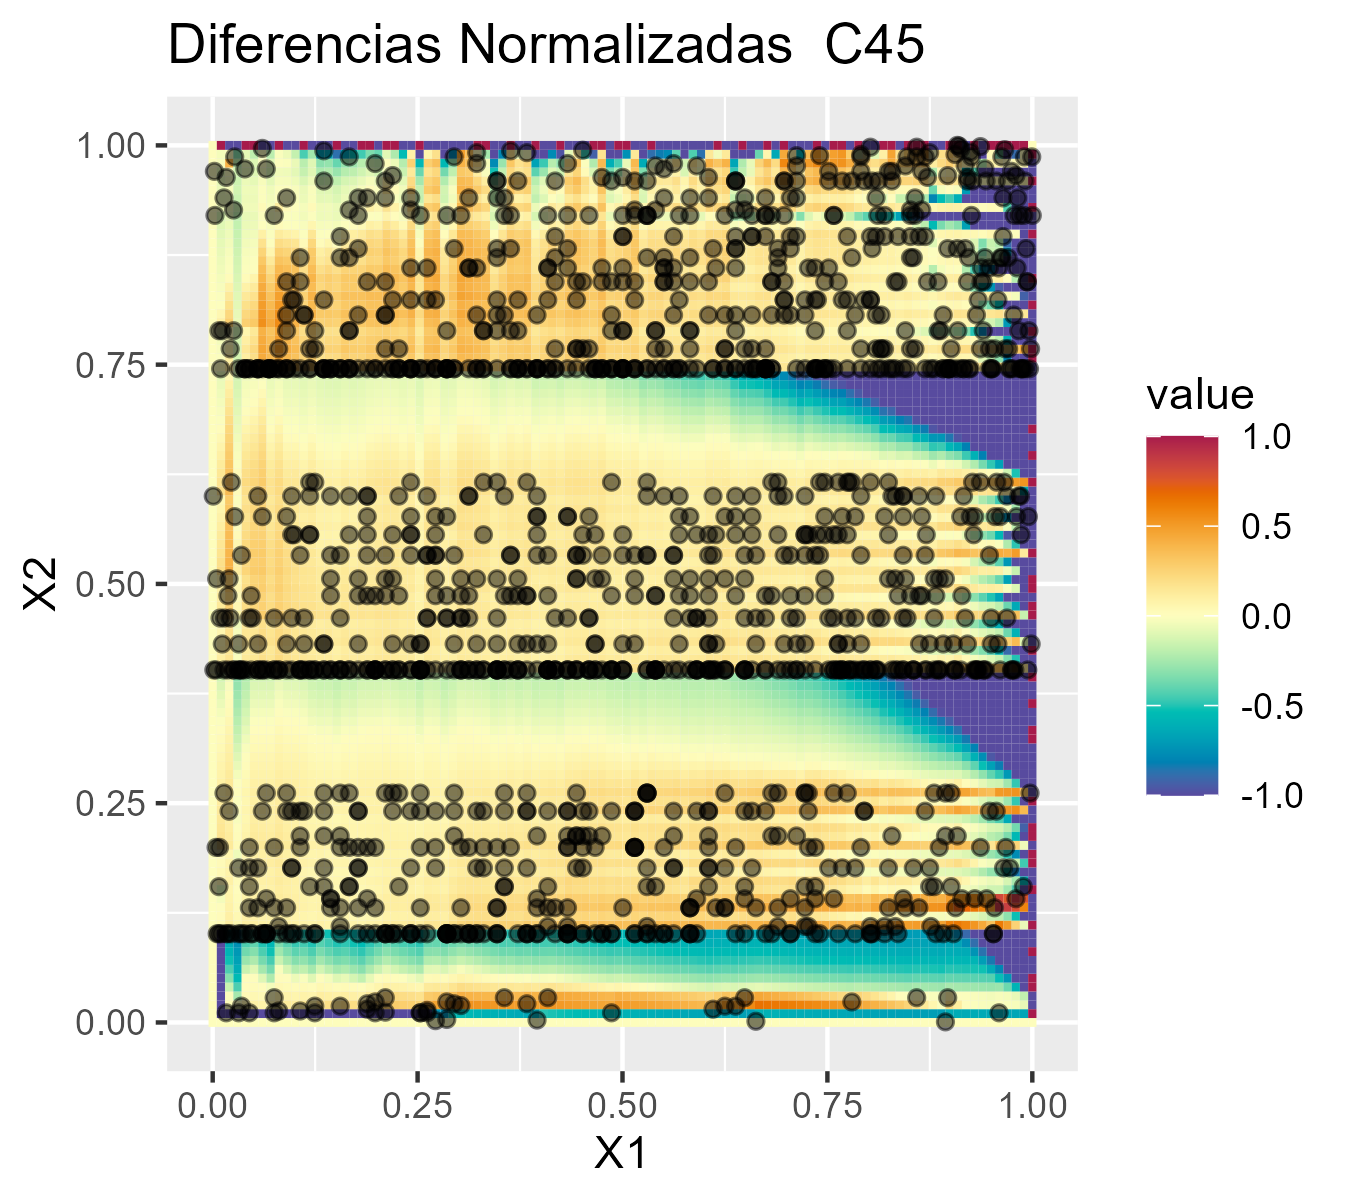
\includegraphics[width=0.3\textwidth]{4img/TotalHC45.png}}
    \caption{Cópulas ajustadas para mujeres y hombres, nivel $1$.}
    \label{fig:Modelo4TotalNivel1}
\end{figure}

Estas gráficas proporcionan una mejor comprensión del tipo y la fuerza de dependencia de cada cópula, y nos permitirá verificar visualmente la monotonicidad de la función para juzgar si el enfoque paramétrico es correcto. Estos heatmaps ayudan a identificar patrones de dependencia y a evaluar la idoneidad del modelo para capturar las relaciones entre las variables.

En la Figura \ref{fig:Modelo4TotalNivel1}, se muestran los heatmaps para cada cópula del nivel $1$. En la cópula $C_{12}$, que modela la relación entre $FBIGC$ y la glucosa al tiempo $120$. No se observa una clara dependencia en la primera parte del dominio, pero posteriormente se evidencia una dependencia de cuadrante negativo. Por otro lado, en la cópula $C_{23}$, que representa la relación entre la glucosa al tiempo $120$ y la glucosa al tiempo $0$, se observa una dependencia de cuadrante positivo que se presenta en todo el dominio. Además, en la cópula $C_{34}$, correspondiente a la glucosa al tiempo $0$ y el Índice de Masa Corporal, se observa una fuerte dependencia de cuadrante positivo.

En cuanto a la cópula $C_{45}$, se observa una relación singular caracterizada por líneas horizontales, que coinciden con los patrones de dispersión vistos en la Figura \ref{fig:diagTot}. Sin embargo, su dependencia fluctúa de positiva a negativa repentinamente, pero su depedencia en las zonas positivas no parece ser muy relevante. Es posible que sea adecuado intentar modelar esta cópula de manera no paramétrica para obtener un modelo más preciso y capturar mejor la complejidad de la relación entre las variables.

%%%%%%%%%%%%%%%%%%%%%%%%%%%%%%%%%%%%%%%%%%%%%%%%

\begin{figure}[H]
 \centering
  \subfloat[$\mathscr{H}\rho_{C_{13|2}}$]{
   \label{C13.2rhoT}
    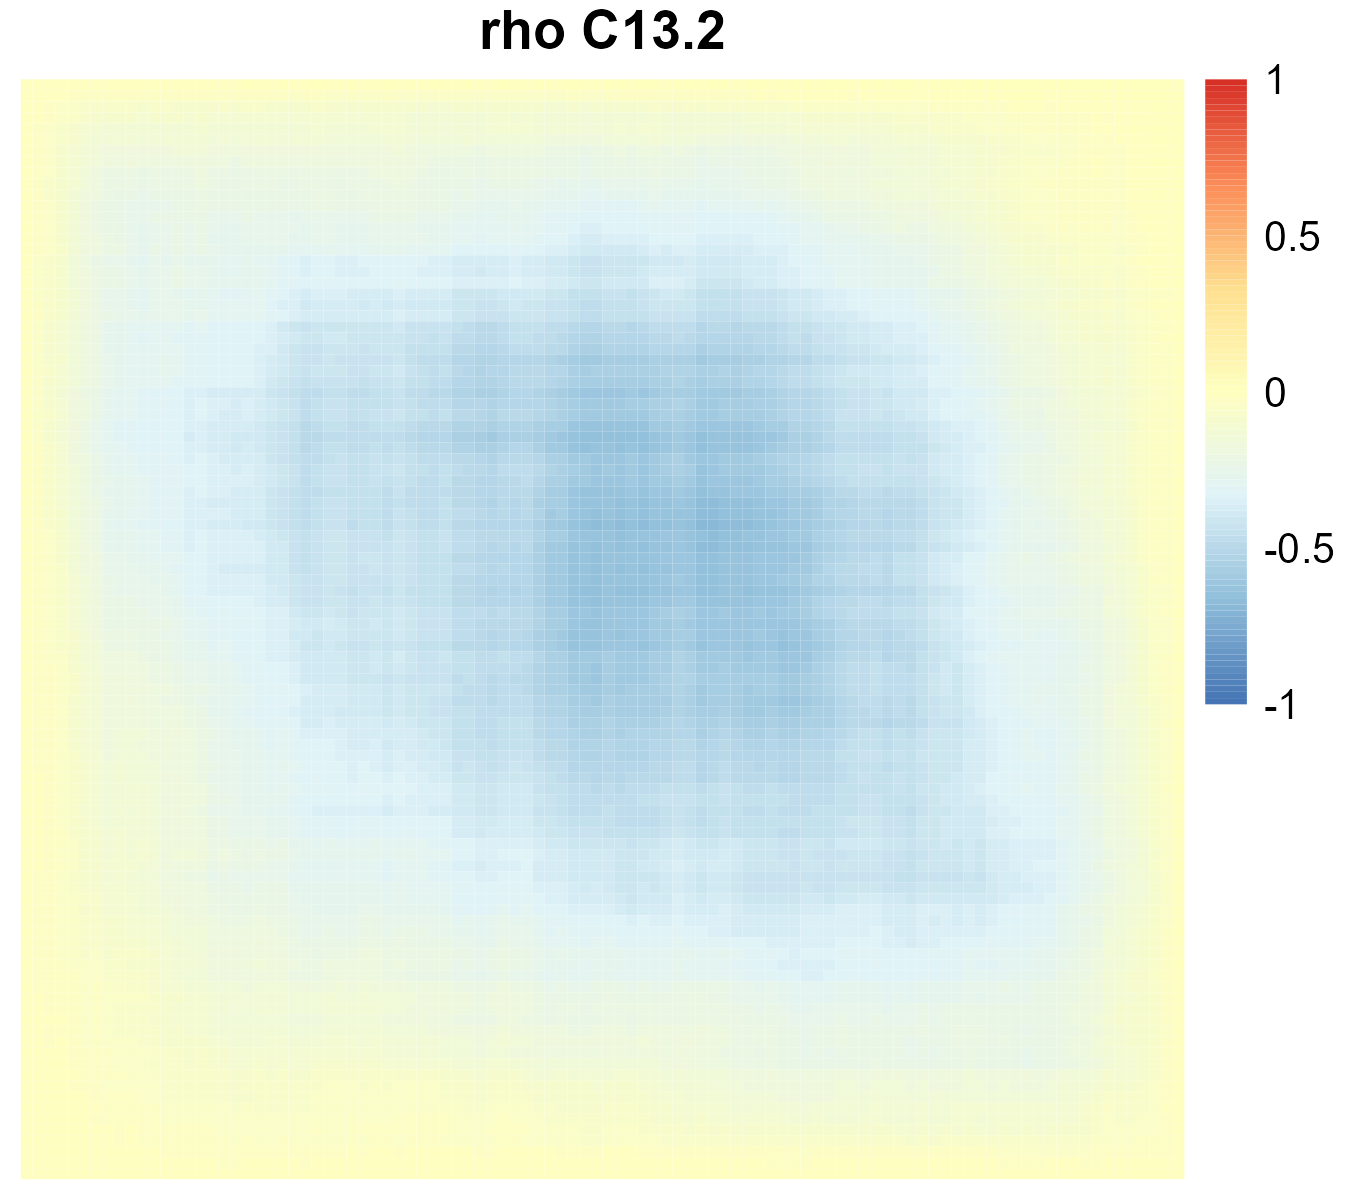
\includegraphics[width=0.33\textwidth]{4img/TotalrhoC13.2.png}}
  \subfloat[$\mathscr{H}\sigma_{C_{13|2}}$]{
   \label{C13.2sigmaT}
    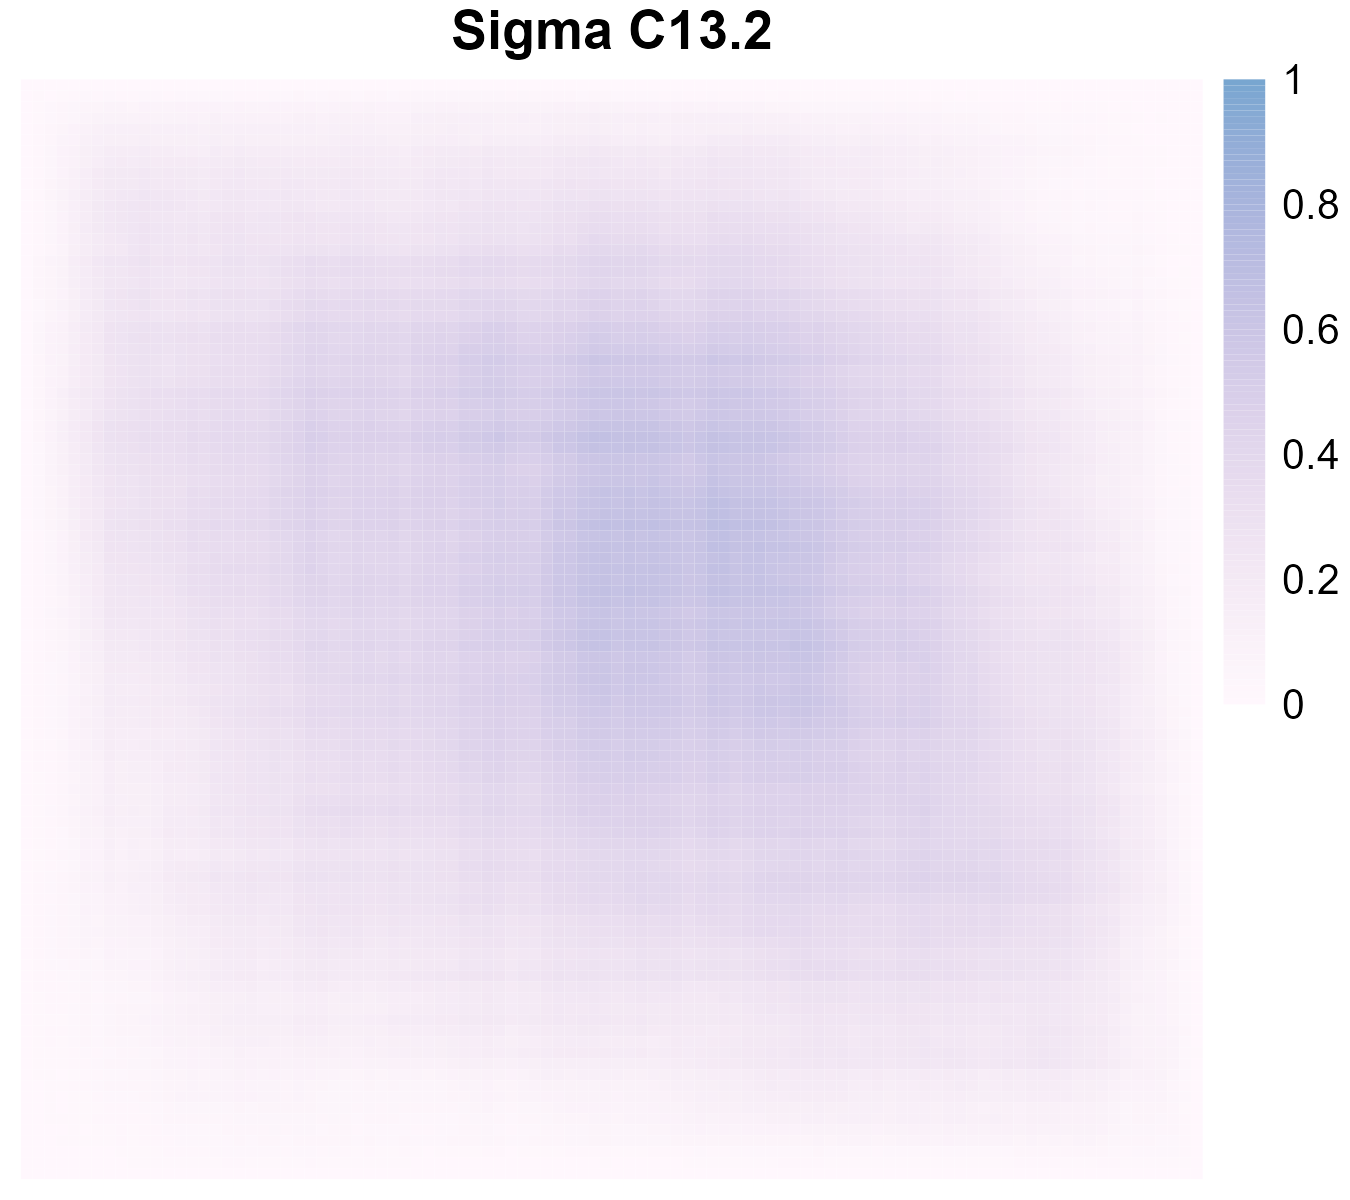
\includegraphics[width=0.33\textwidth]{4img/TotalsigmaC13.2.png}}
  \subfloat[$\mathscr{H}_{C_{13|2}}$]{
   \label{C13.2HT}
    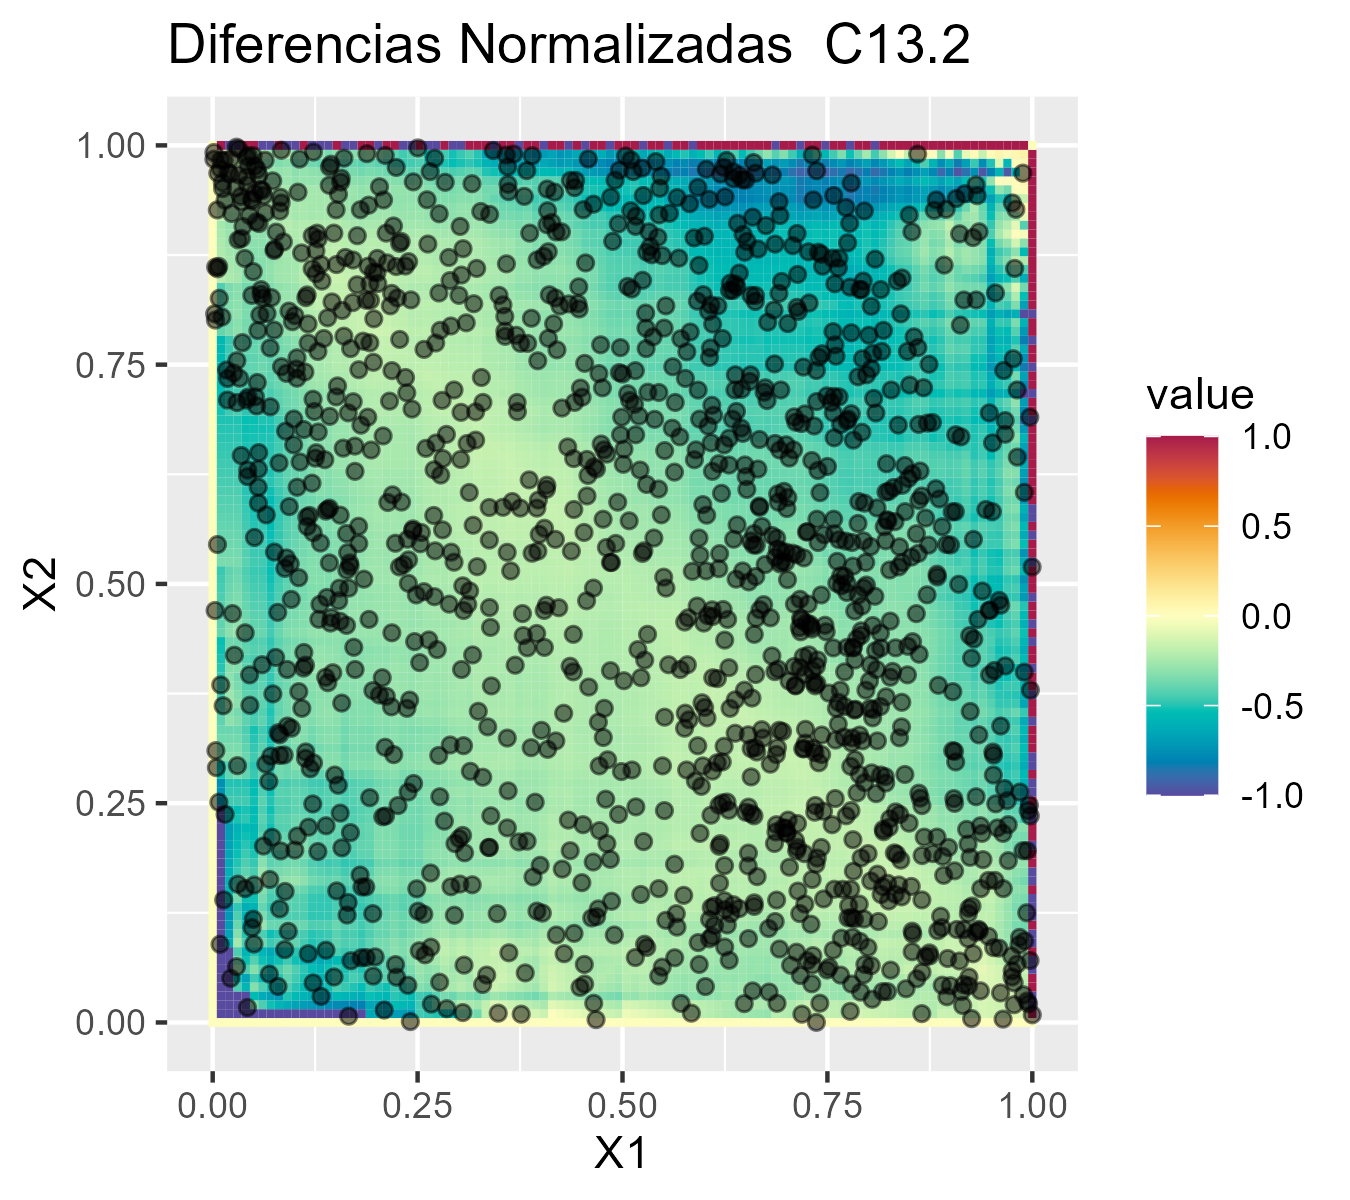
\includegraphics[width=0.33\textwidth]{4img/TotalHC13.2.png}}
\end{figure}

\begin{figure}[H]
 \centering
  \subfloat[$\mathscr{H}\rho_{C_{24|3}}$]{
   \label{C24.3rhoT}
    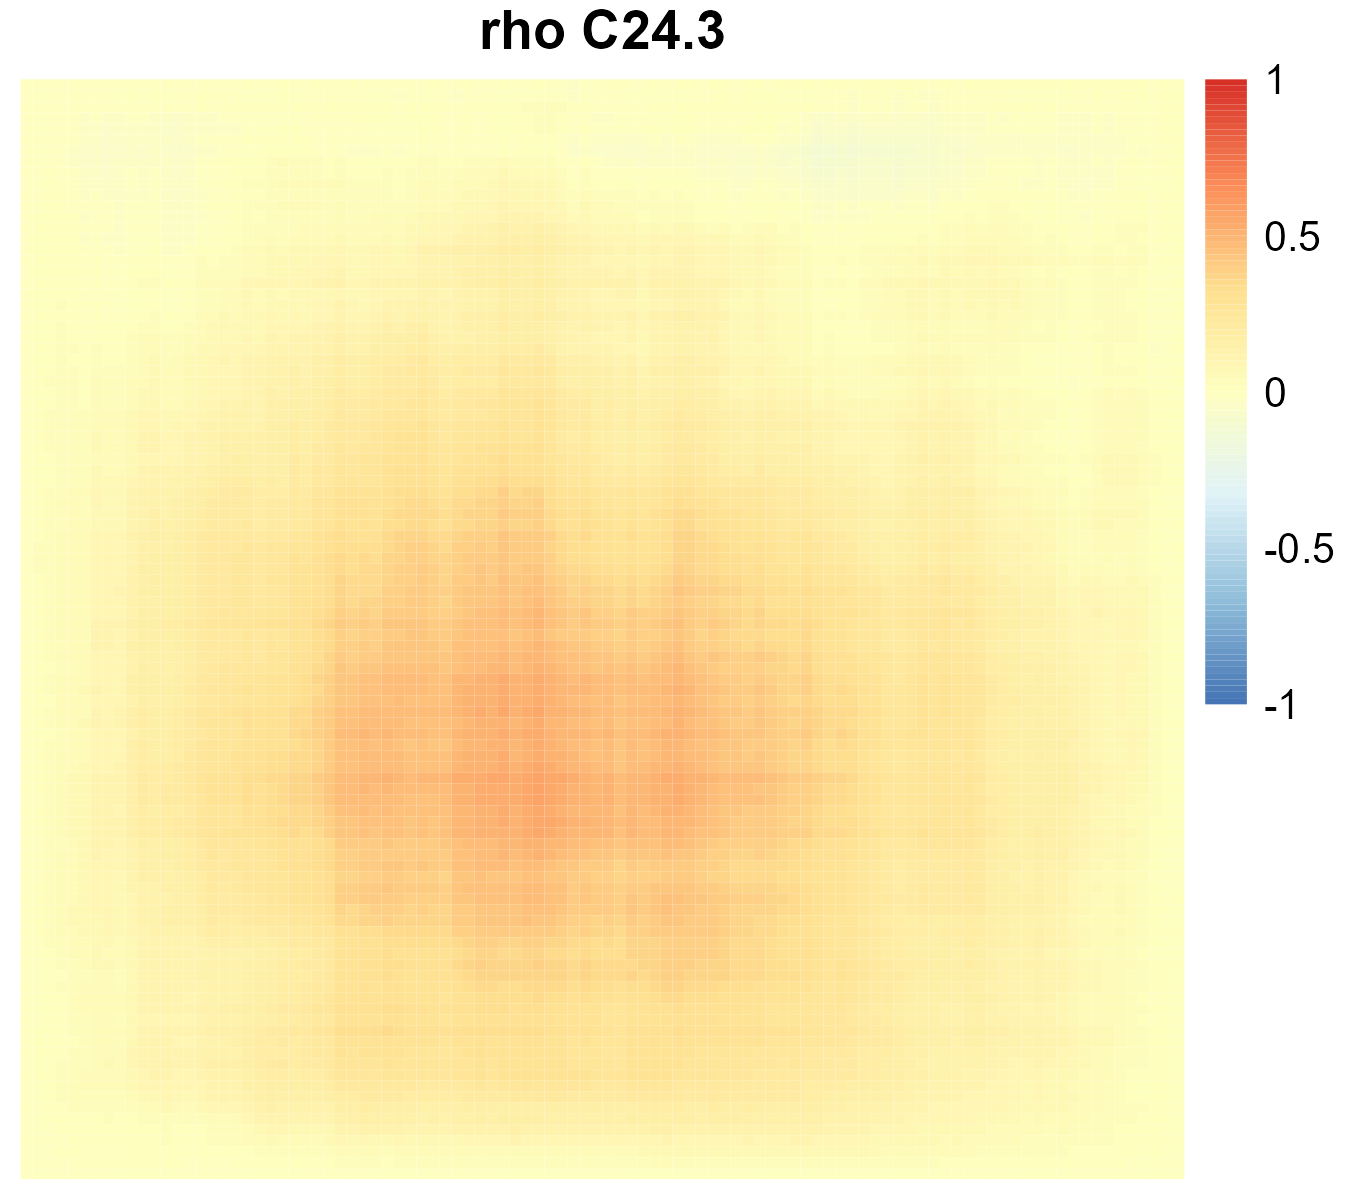
\includegraphics[width=0.33\textwidth]{4img/TotalrhoC24.3.png}}
  \subfloat[$\mathscr{H}\sigma_{C_{24|3}}$]{
   \label{C24.3sigmaT}
    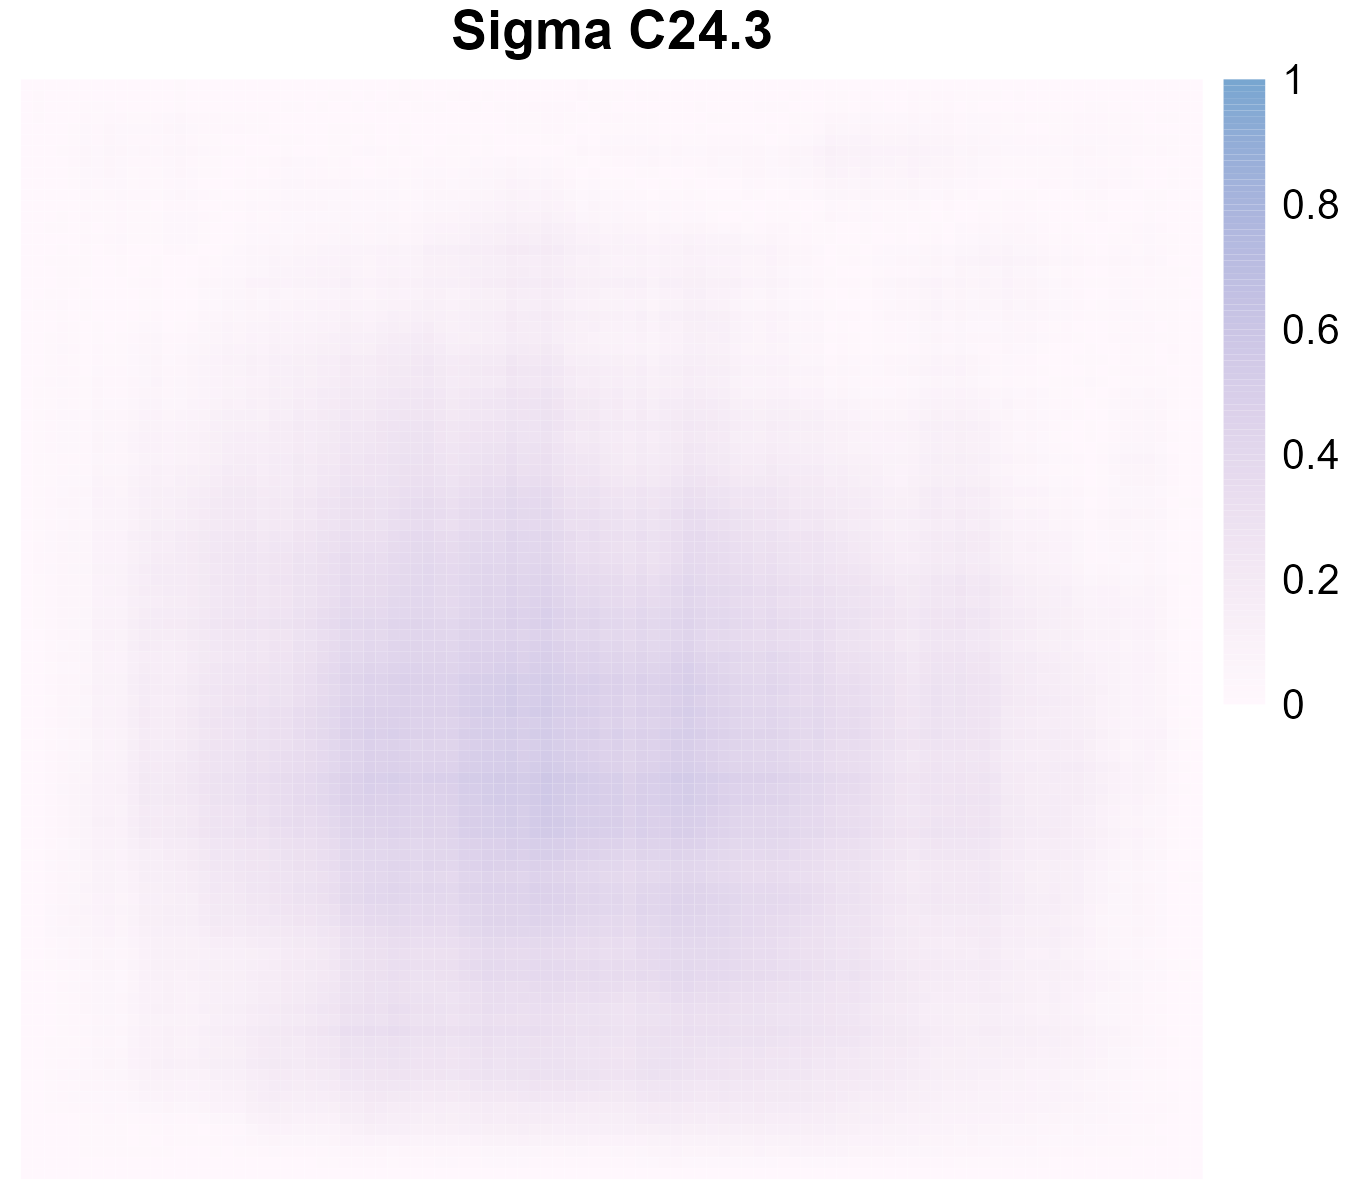
\includegraphics[width=0.33\textwidth]{4img/TotalsigmaC24.3.png}}
  \subfloat[$\mathscr{H}_{C_{24|3}}$]{
   \label{C24.3HT}
    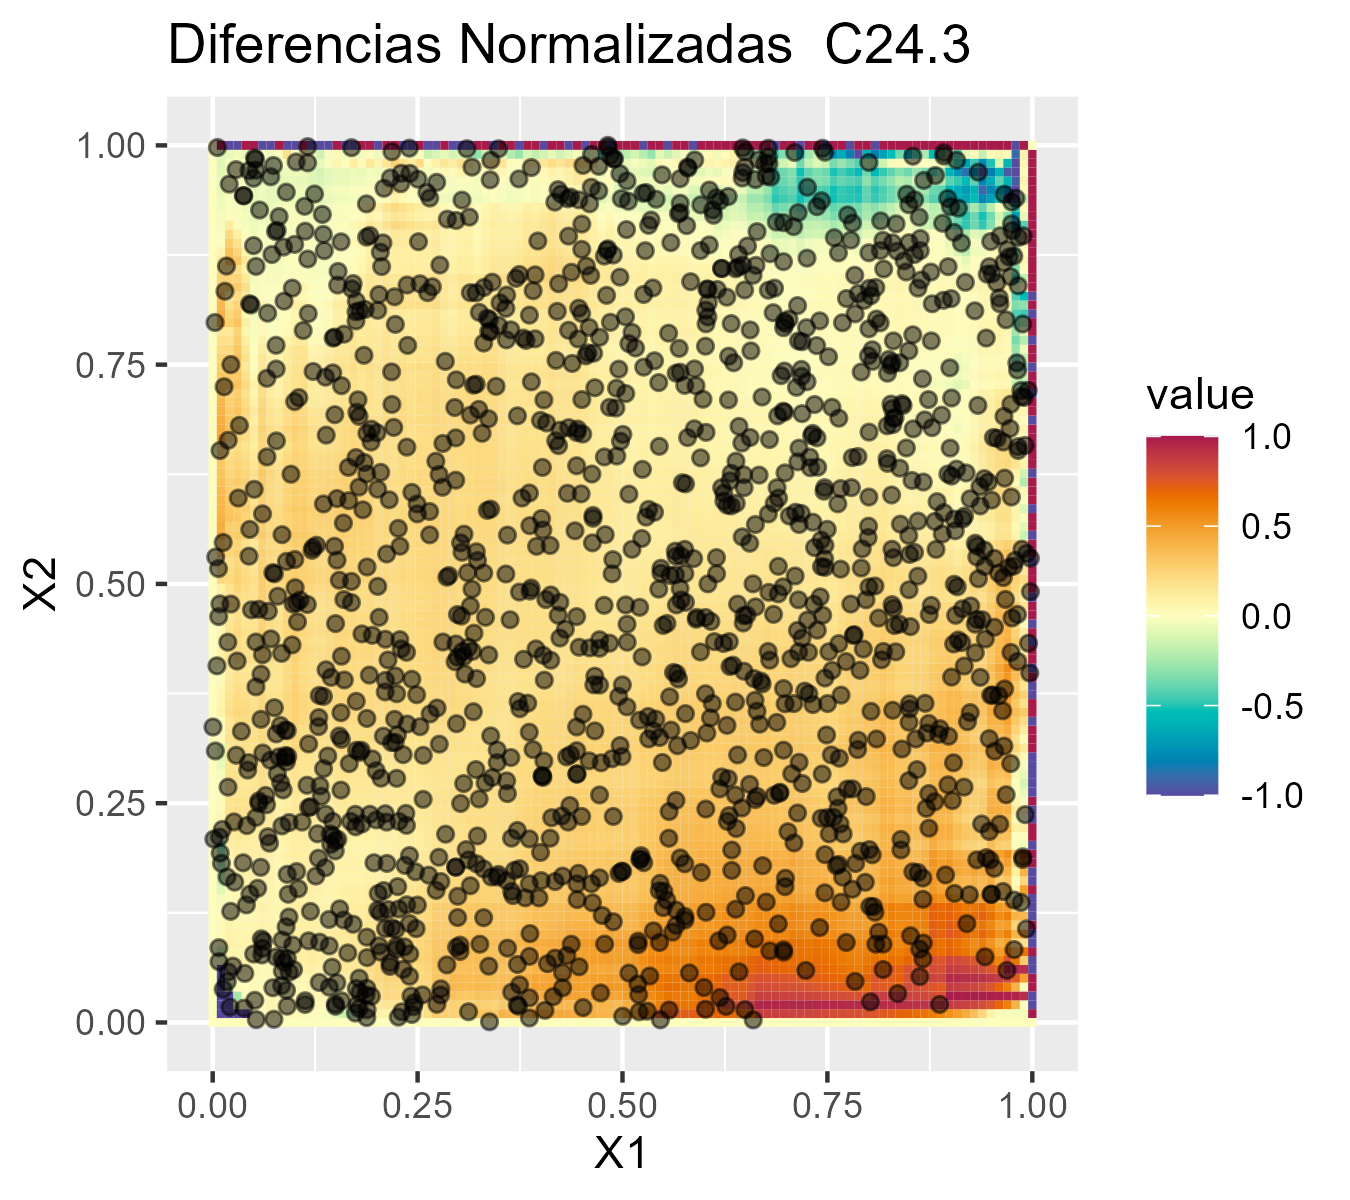
\includegraphics[width=0.33\textwidth]{4img/TotalHC24.3.png}}
\end{figure}

\begin{figure}[H]
 \centering
  \subfloat[$\mathscr{H}\rho_{C_{35|4}}$]{
   \label{C35.4rhoT}
    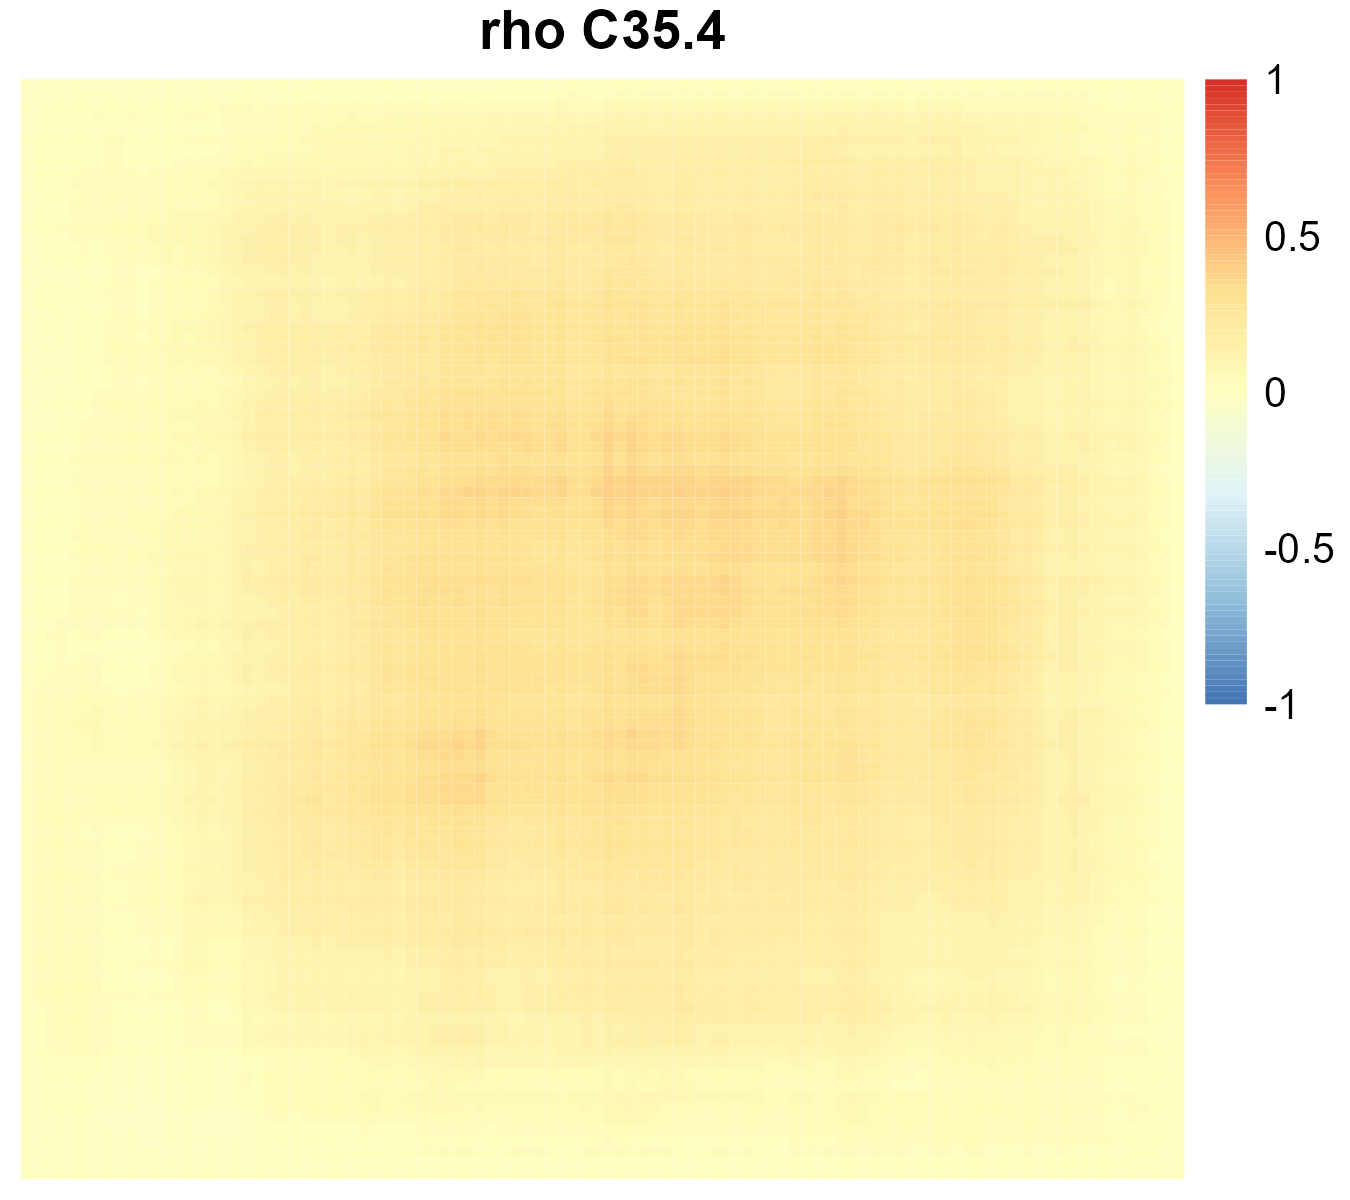
\includegraphics[width=0.33\textwidth]{4img/TotalrhoC35.4.png}}
  \subfloat[$\mathscr{H}\sigma_{C_{35|4}}$]{
   \label{C35.4sigmaT}
    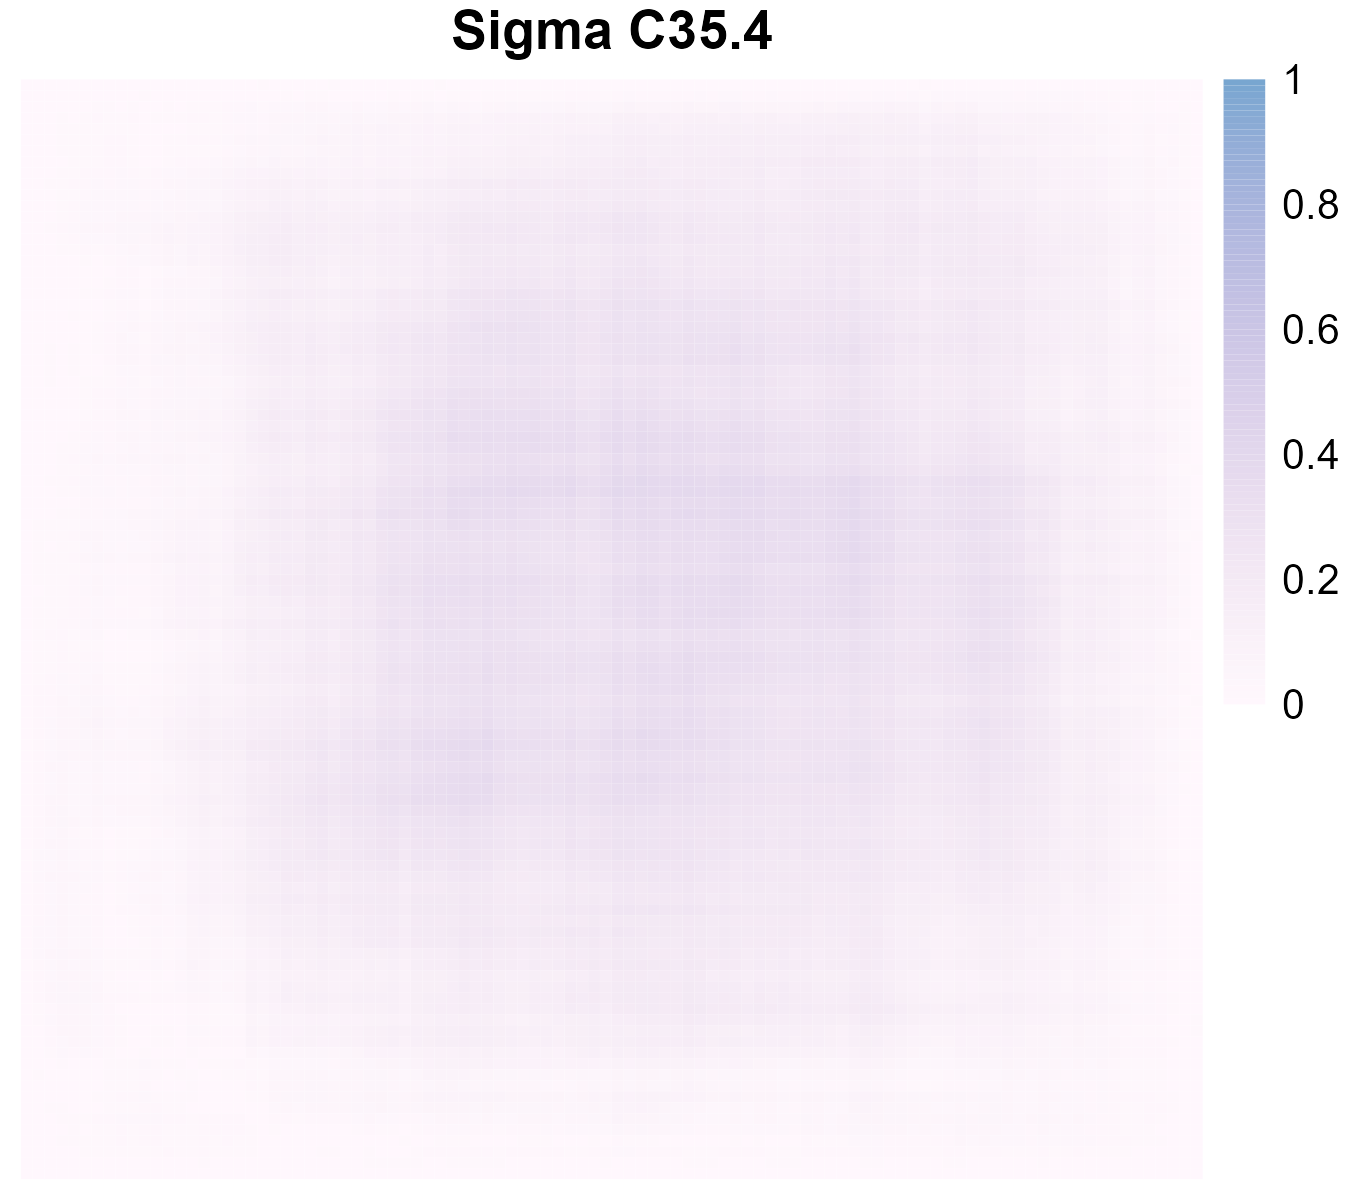
\includegraphics[width=0.33\textwidth]{4img/TotalsigmaC35.4.png}}
  \subfloat[$\mathscr{H}_{C_{35|4}}$]{
   \label{C35.4HT}
    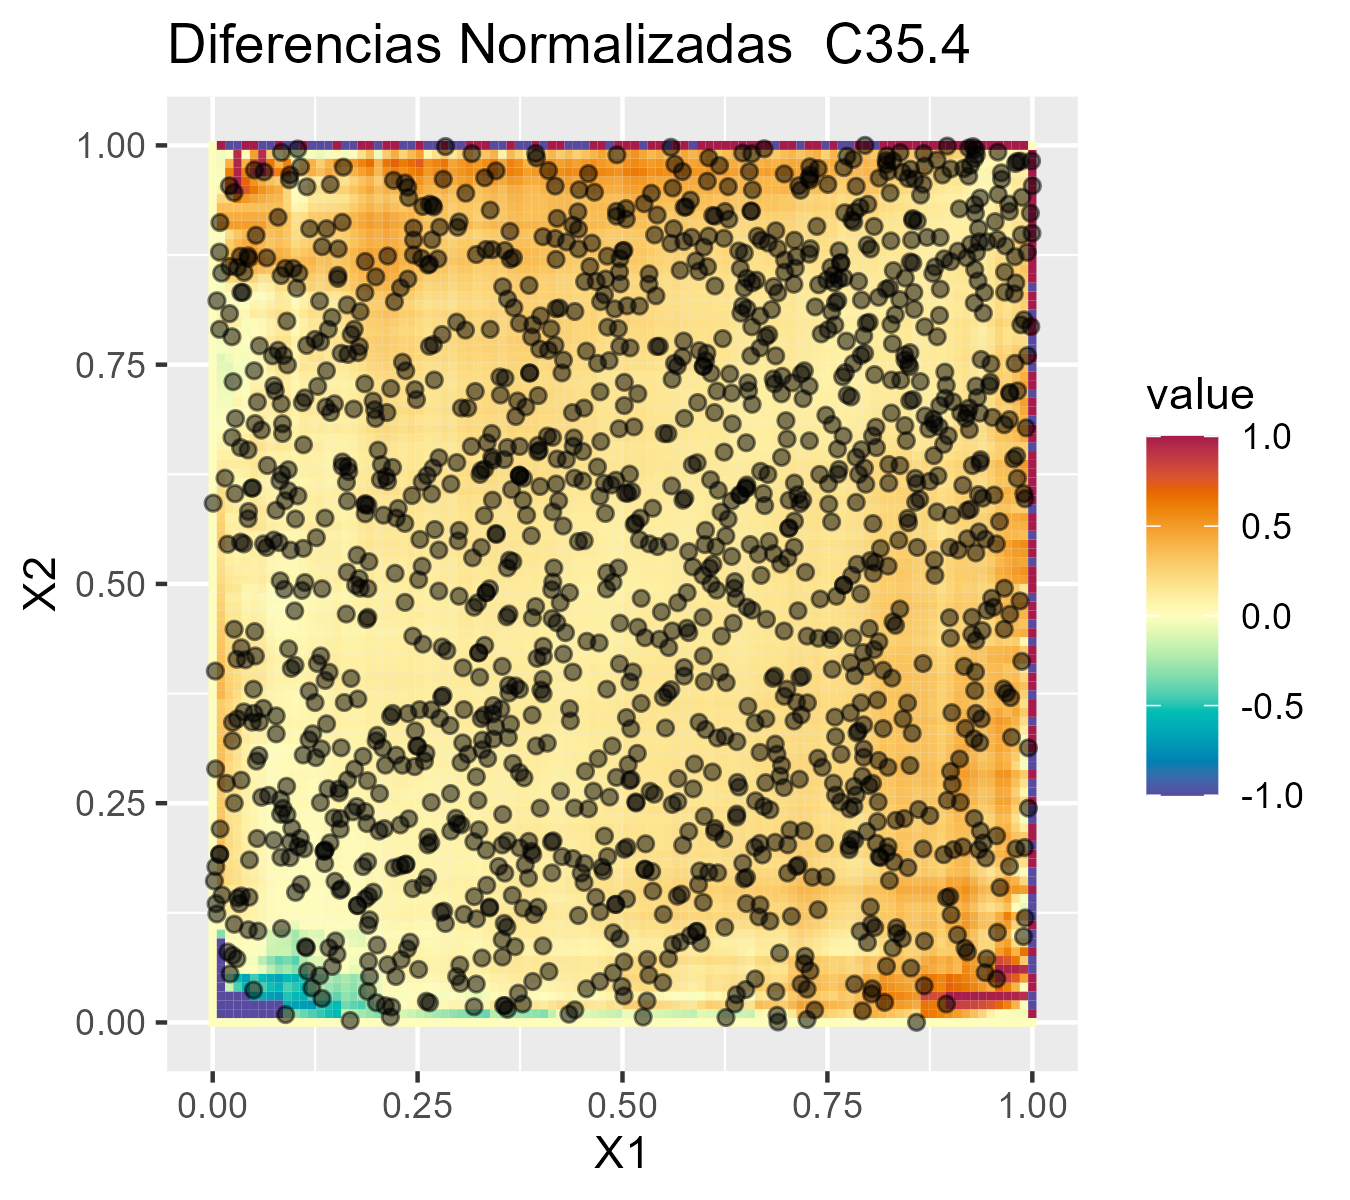
\includegraphics[width=0.33\textwidth]{4img/TotalHC35.4.png}}
    \caption{Cópulas ajustadas para mujeres y hombres, nivel $2$.}
    \label{fig:Modelo4TotalNivel2}
\end{figure}

En la Figura \ref{fig:Modelo4TotalNivel2} se muestran las cópulas del nivel $2$. La primera cópula, $C_{13|2}$, corresponde a la variable respuesta y la medición de glucosa al tiempo $0$ condicionada a la glucosa al tiempo $120$. Se observa una relación de dependencia de cuadrante negativo, lo cual tiene sentido porque cuanto más baja es la variable respuesta, es posible que el cuerpo tenga dificultades para procesar el azúcar, lo que puede resultar en niveles altos de glucosa. Esta relación sugiere una posible asociación entre la variable respuesta y los niveles de glucosa al tiempo $0$ condicionados por los niveles de glucosa al tiempo 120, lo cual es coherente con el conocimiento médico sobre la fisiología del metabolismo del azúcar en el cuerpo.

La cópula $C_{24|3}$, que representa la relación entre la medición de glucosa al tiempo $120$ y el índice de masa corporal condicionado a los niveles de glucosa al tiempo $0$, muestra una relación de dependencia de cuadrante positiva, lo cual tiene sentido desde un punto de vista médico. Esto sugiere que a medida que los niveles de glucosa al tiempo $120$ aumentan, también tiende a aumentar el índice de masa corporal.

La relación entre la glucosa al tiempo $0$ y la presión diastólica, condicionada al índice de masa corporal, corresponde a la cópula $C_{35|4}$. Al observar una dependencia de cuadrante positiva, se esperaría que un aumento en los niveles de glucosa al tiempo $0$ esté asociado con una disminución en los valores de presión diastólica. Sin embargo, es importante ser cauteloso al interpretar esta relación, ya que puede estar influida por la distribución singular que se observó en la cópula $C_{45}$.

%%%%%%%%%%%%%%%%%%%%%%%%%%%%%%%%%%%%%%%%%%%%%%%%%%

\begin{figure}[H]
 \centering
  \subfloat[$\mathscr{H}\rho_{C_{14|23}}$]{
   \label{C14.23rhoT}
    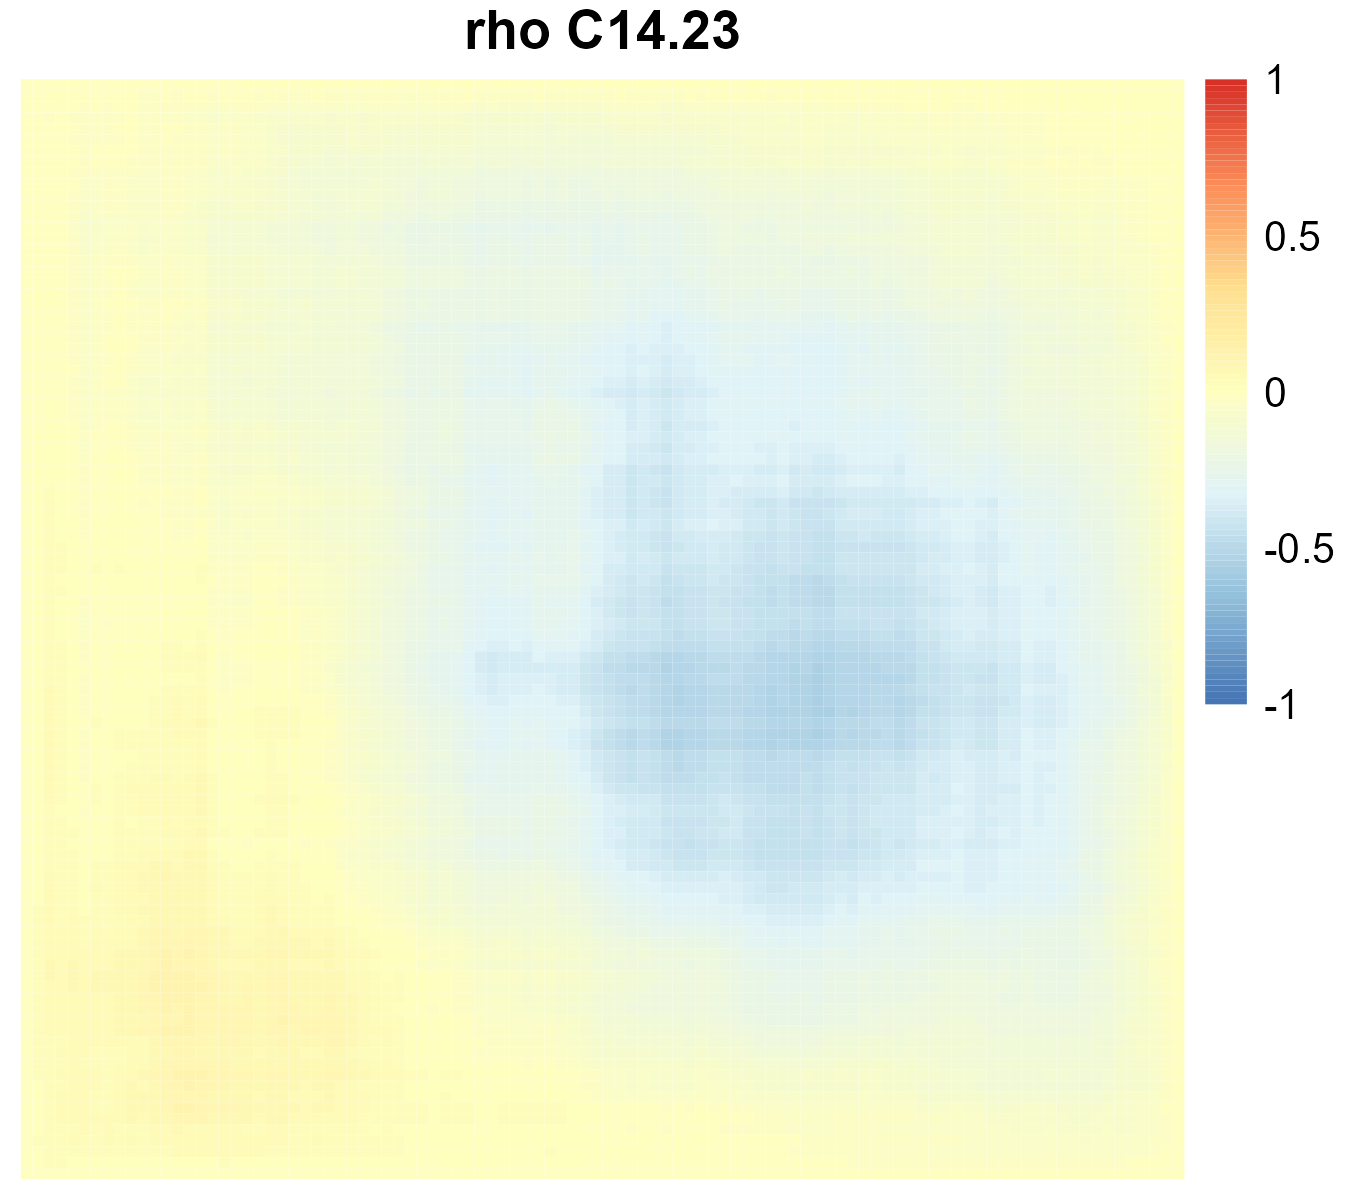
\includegraphics[width=0.3\textwidth]{4img/TotalrhoC14.23.png}}
  \subfloat[$\mathscr{H}\sigma_{C_{14|23}}$]{
   \label{C14.23sigmaT}
    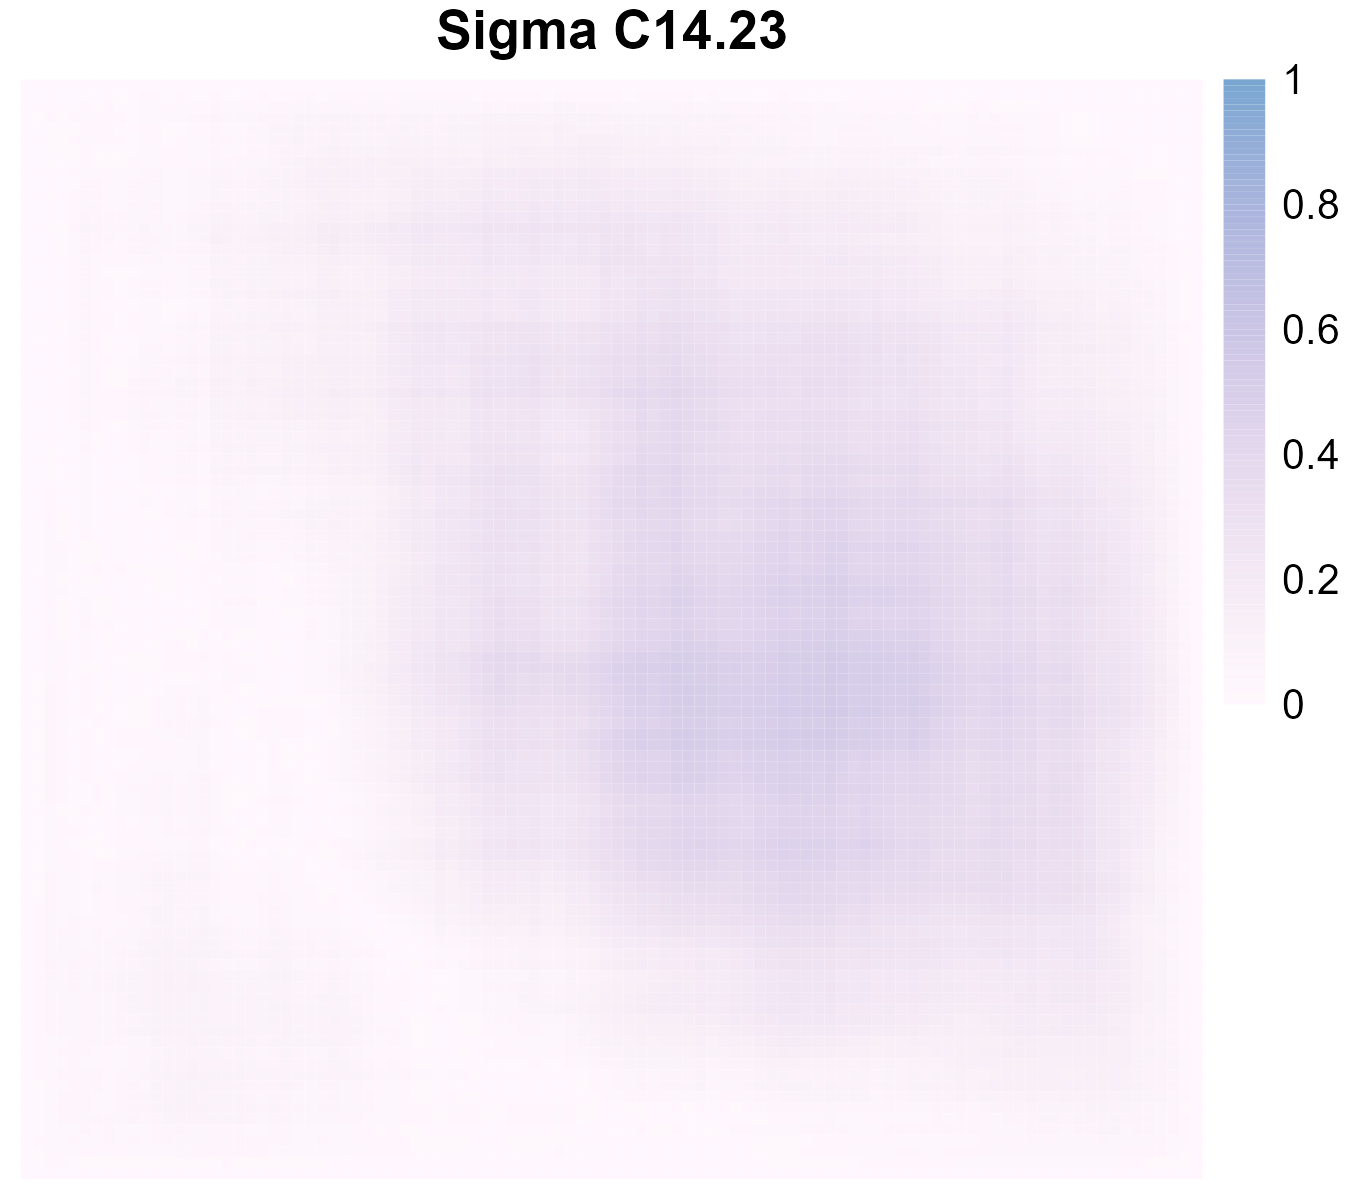
\includegraphics[width=0.3\textwidth]{4img/TotalsigmaC14.23.png}}
  \subfloat[$\mathscr{H}_{C_{14|23}}$]{
   \label{C14.23HT}
    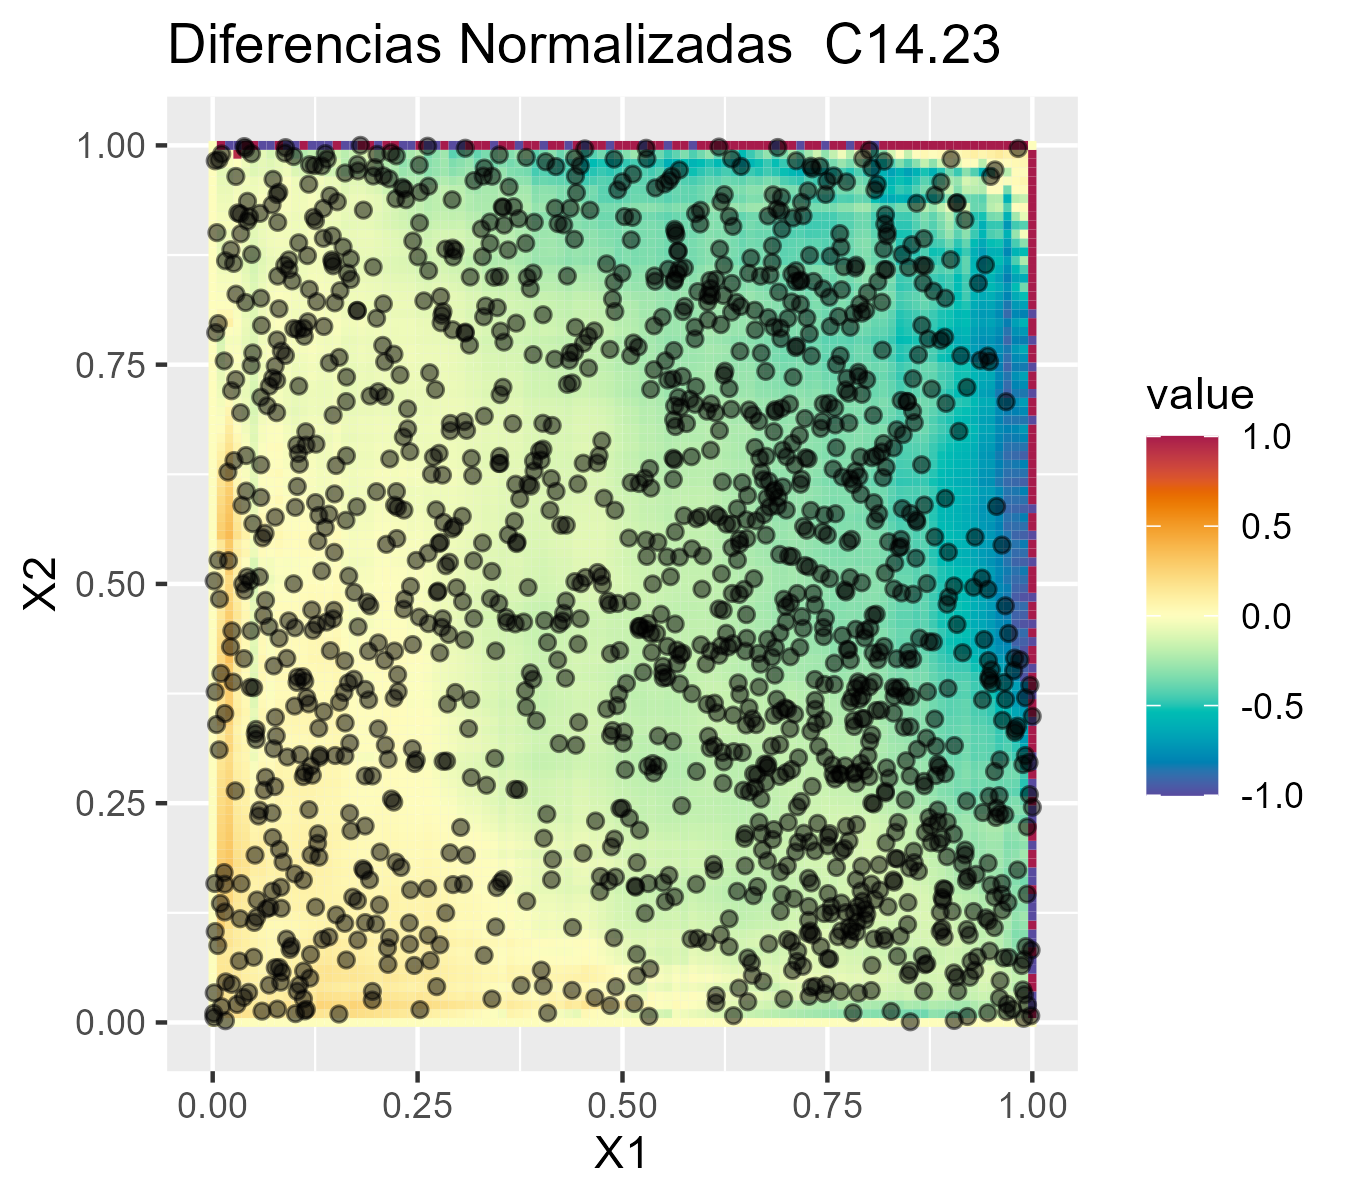
\includegraphics[width=0.3\textwidth]{4img/TotalHC14.23.png}}
\end{figure}

\begin{figure}[H]
 \centering
  \subfloat[$\mathscr{H}\rho_{C_{25|34}}$]{
   \label{C25.34rhoT}
    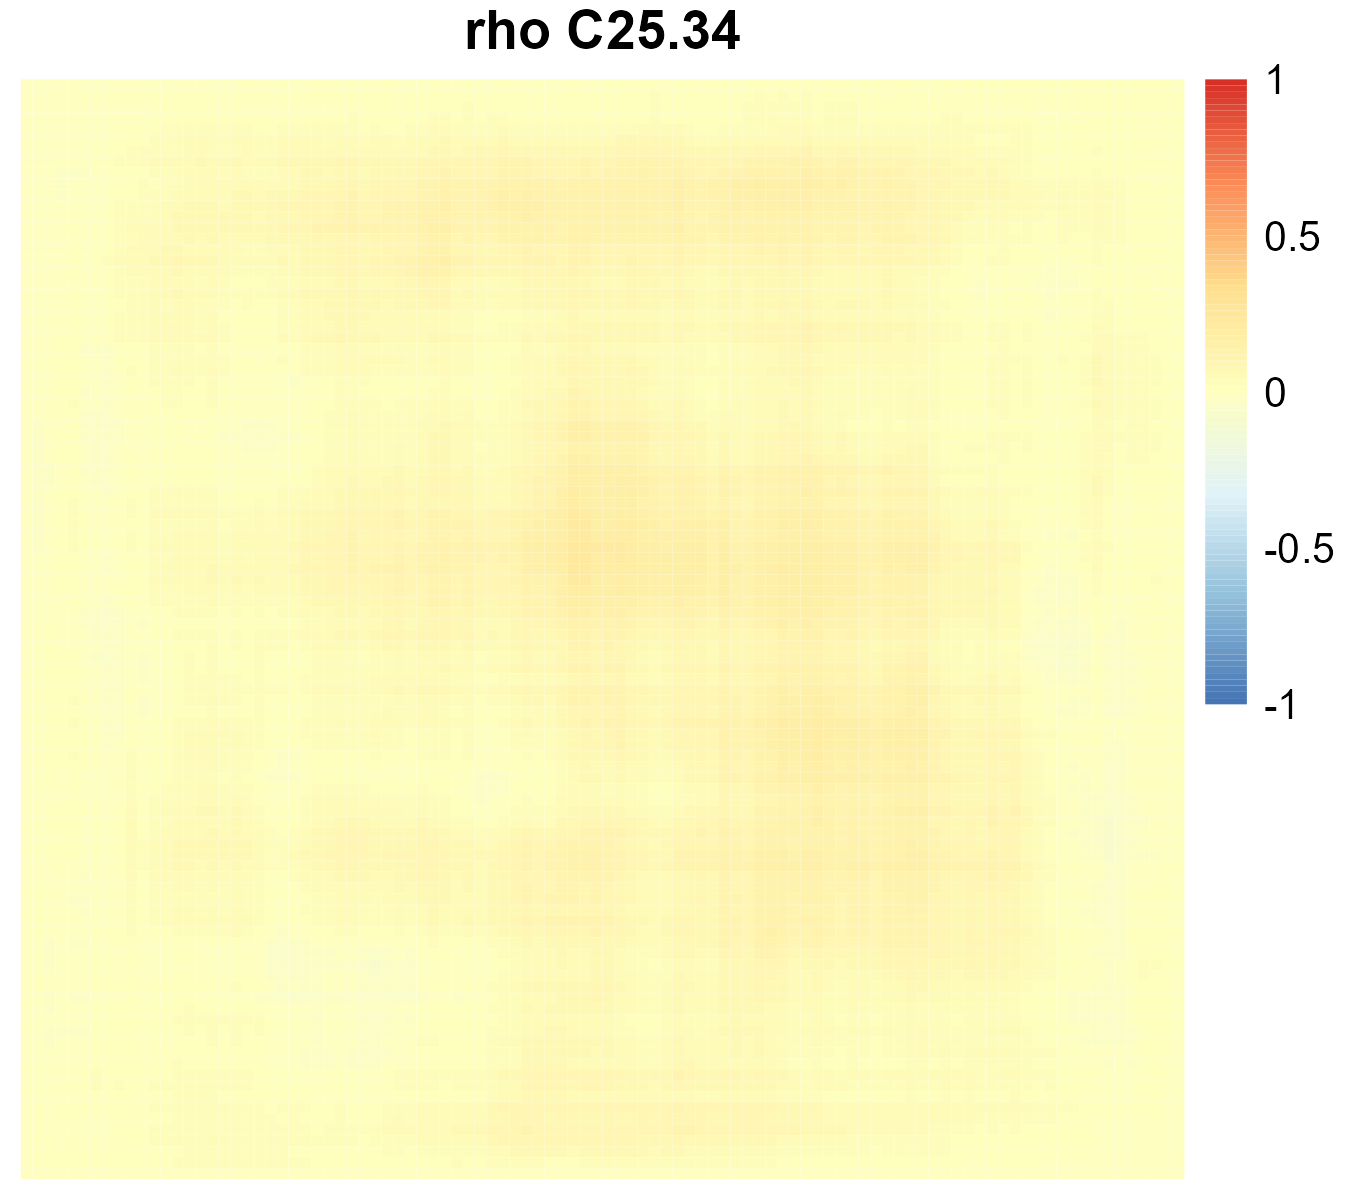
\includegraphics[width=0.3\textwidth]{4img/TotalrhoC25.34.png}}
  \subfloat[$\mathscr{H}\sigma_{C_{25|34}}$]{
   \label{C25.34sigmaT}
    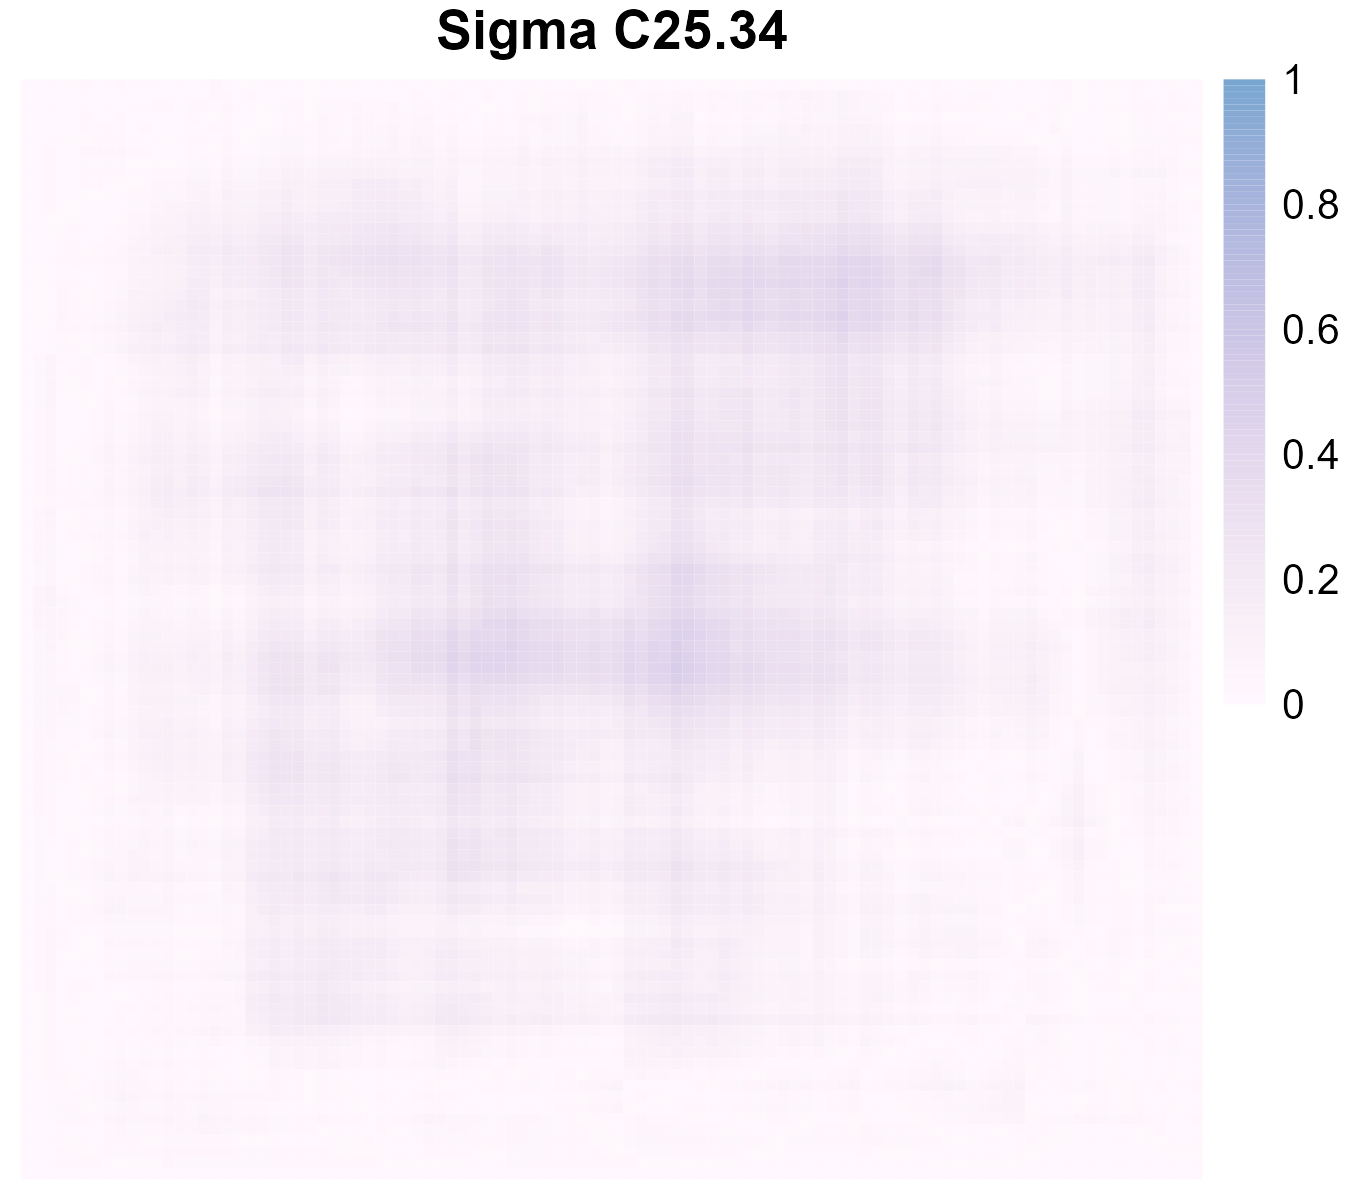
\includegraphics[width=0.3\textwidth]{4img/HomsigmaC25.34.png}}
  \subfloat[$\mathscr{H}_{C_{25|34}}$]{
   \label{C25.34HT}
    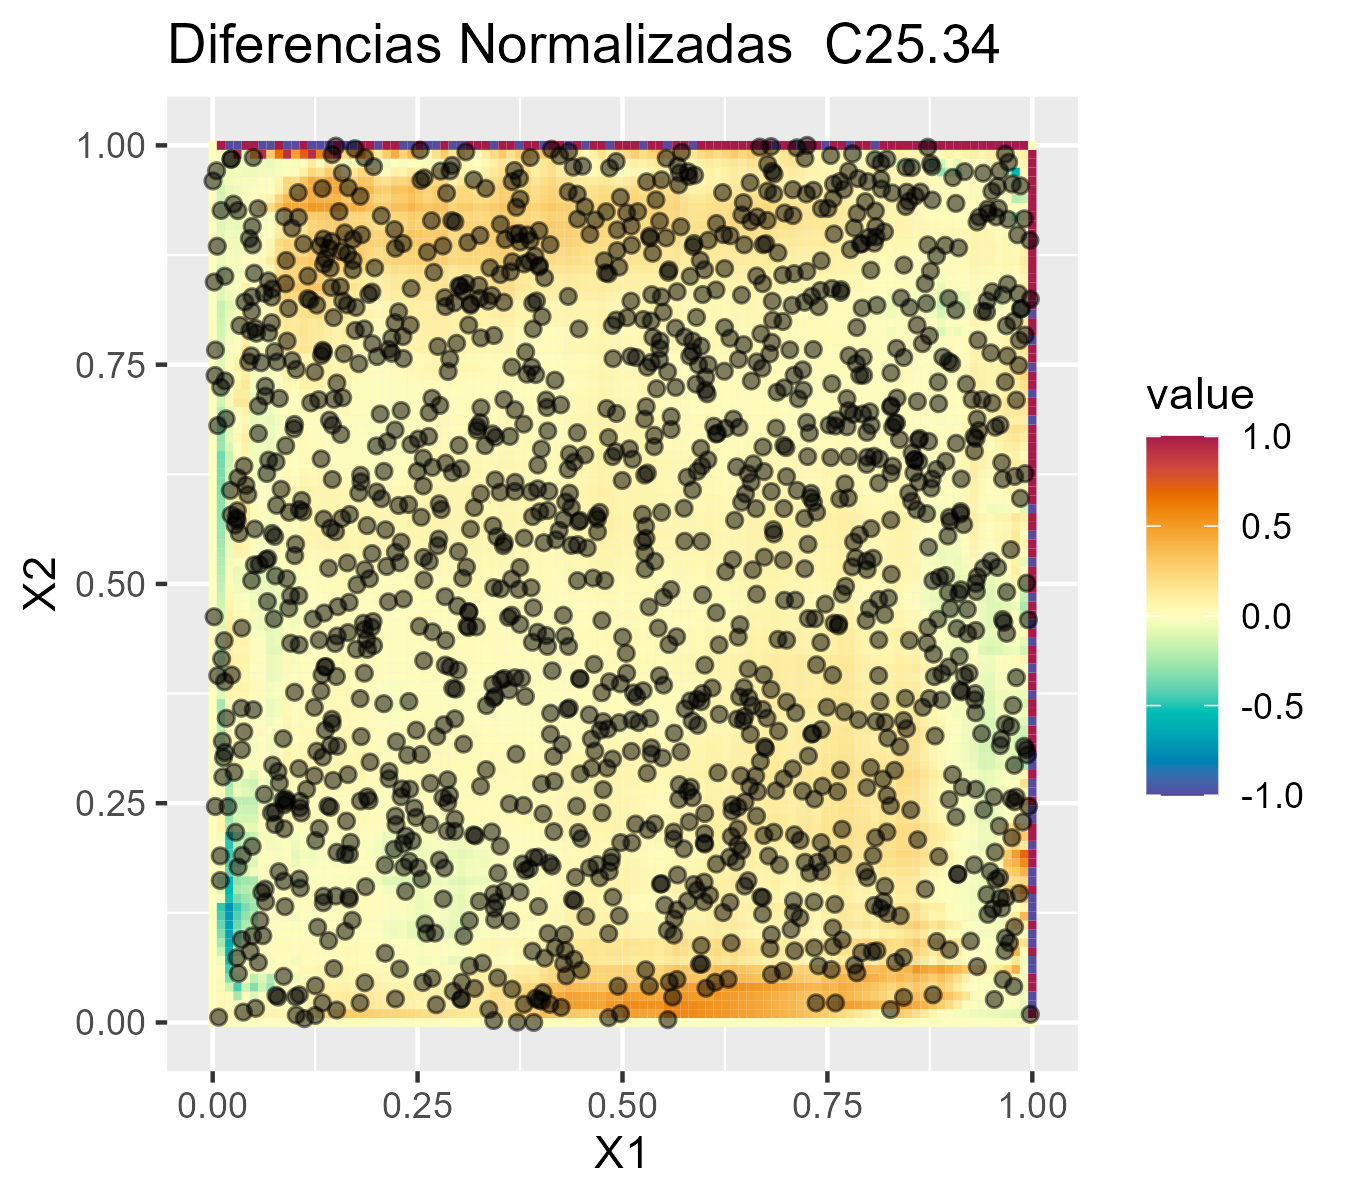
\includegraphics[width=0.3\textwidth]{4img/TotalHC25.34.png}}
    \caption{Cópulas ajustadas para mujeres y hombres, nivel $3$.}
    \label{fig:Modelo4TotalNivel3}
\end{figure}


Las cópula de nivel $3$ se muestran en la Figura \ref{fig:Modelo4TotalNivel3}. La cópula $C_{14|23}$, que representa la relación entre la variable respuesta y el índice de masa corporal condicionado a los niveles de glucosa al tiempo $0$ y $120$, muestra una baja concordancia. Esta relación se observa como negativa, y cuando el índice de masa corporal es bajo, parece haber independencia. Por otro lado, la cópula $C_{25|34}$ muestra una dependencia muy baja, lo cual está respaldado por los tests de independencia, lo que sugiere que la variable $5$ podría ser potencialmente desechada.

%%%%%%%%%%%%%%%%%%%%%%%%%%%%%%%%%%%%%%%%%%%%%%%%%%


\begin{figure}[H]
 \centering
  \subfloat[$\mathscr{H}\rho_{C_{15|234}}$]{
   \label{C15.234rhoT}
    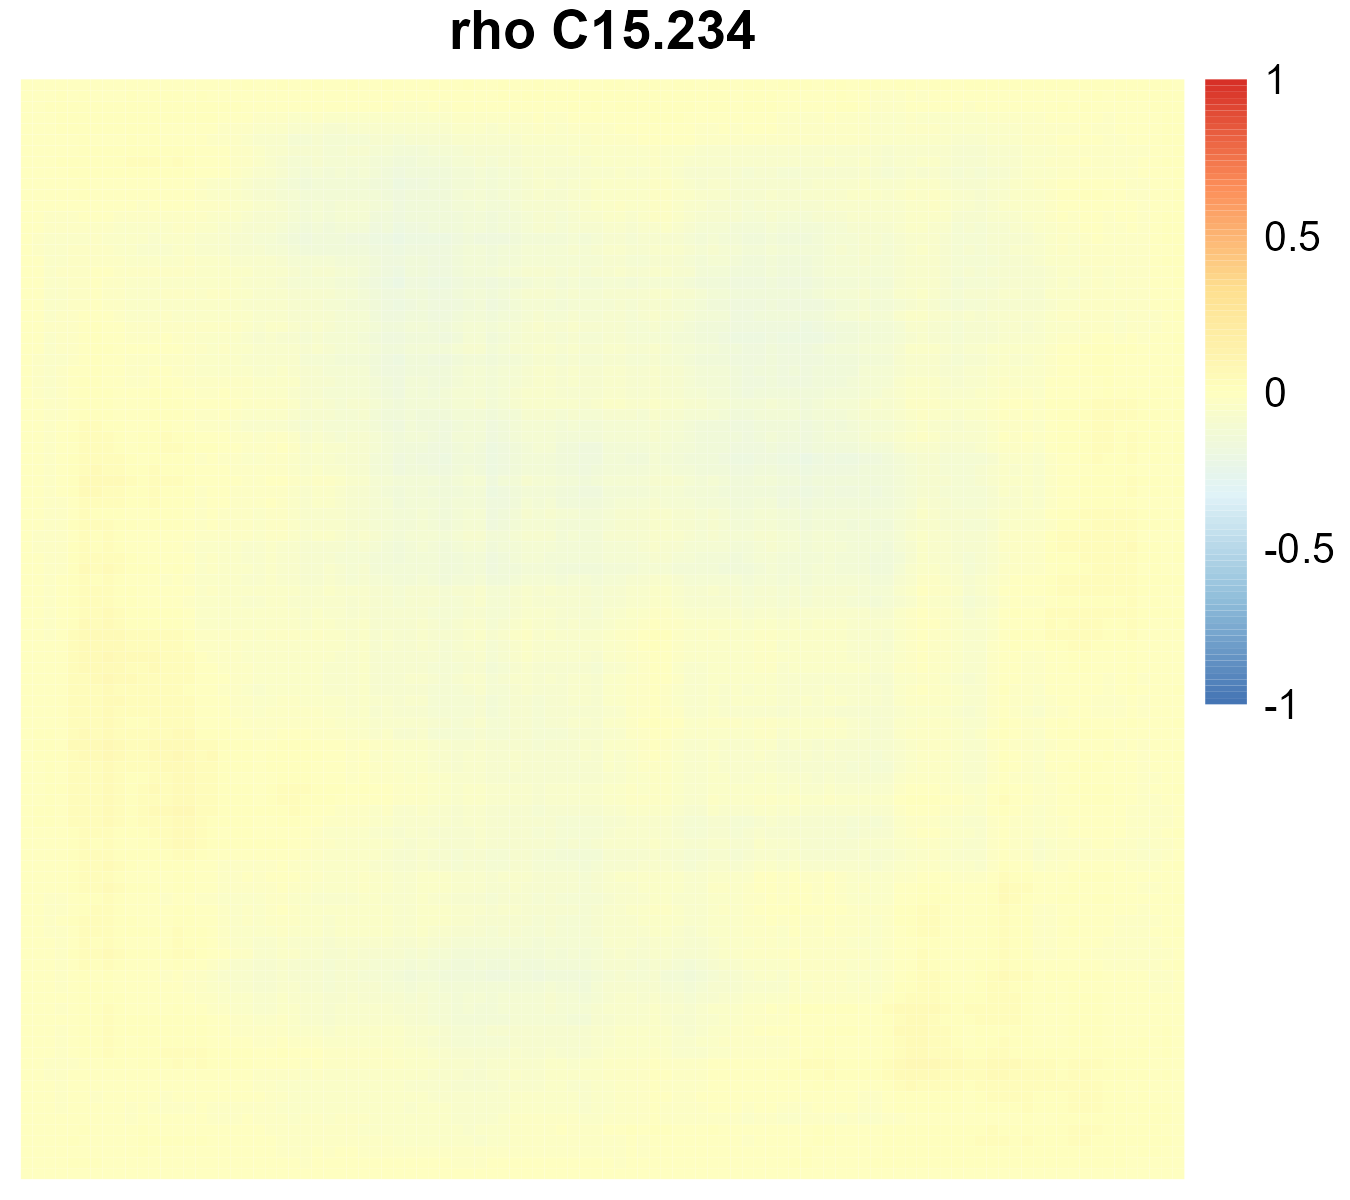
\includegraphics[width=0.3\textwidth]{4img/TotalrhoC15.234.png}}
  \subfloat[$\mathscr{H}\sigma_{C_{15|234}}$]{
   \label{C15.234sigmaT}
    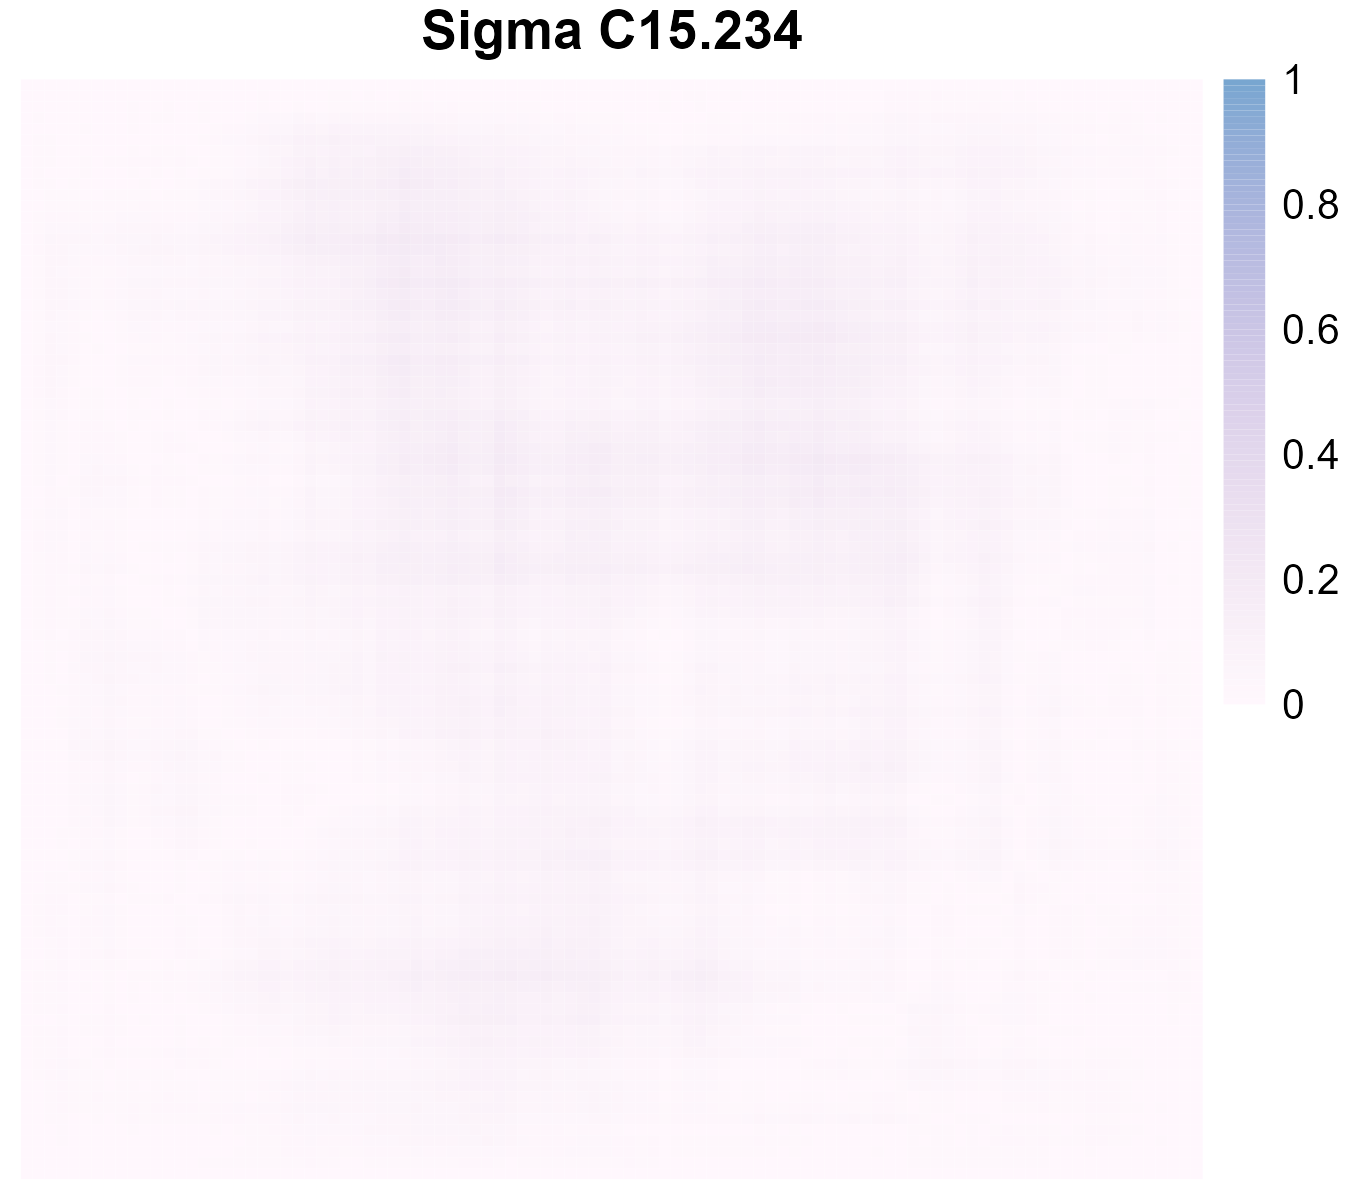
\includegraphics[width=0.3\textwidth]{4img/TotalsigmaC15.234.png}}
  \subfloat[$\mathscr{H}_{C_{15|234}}$]{
   \label{C15.234HT}
    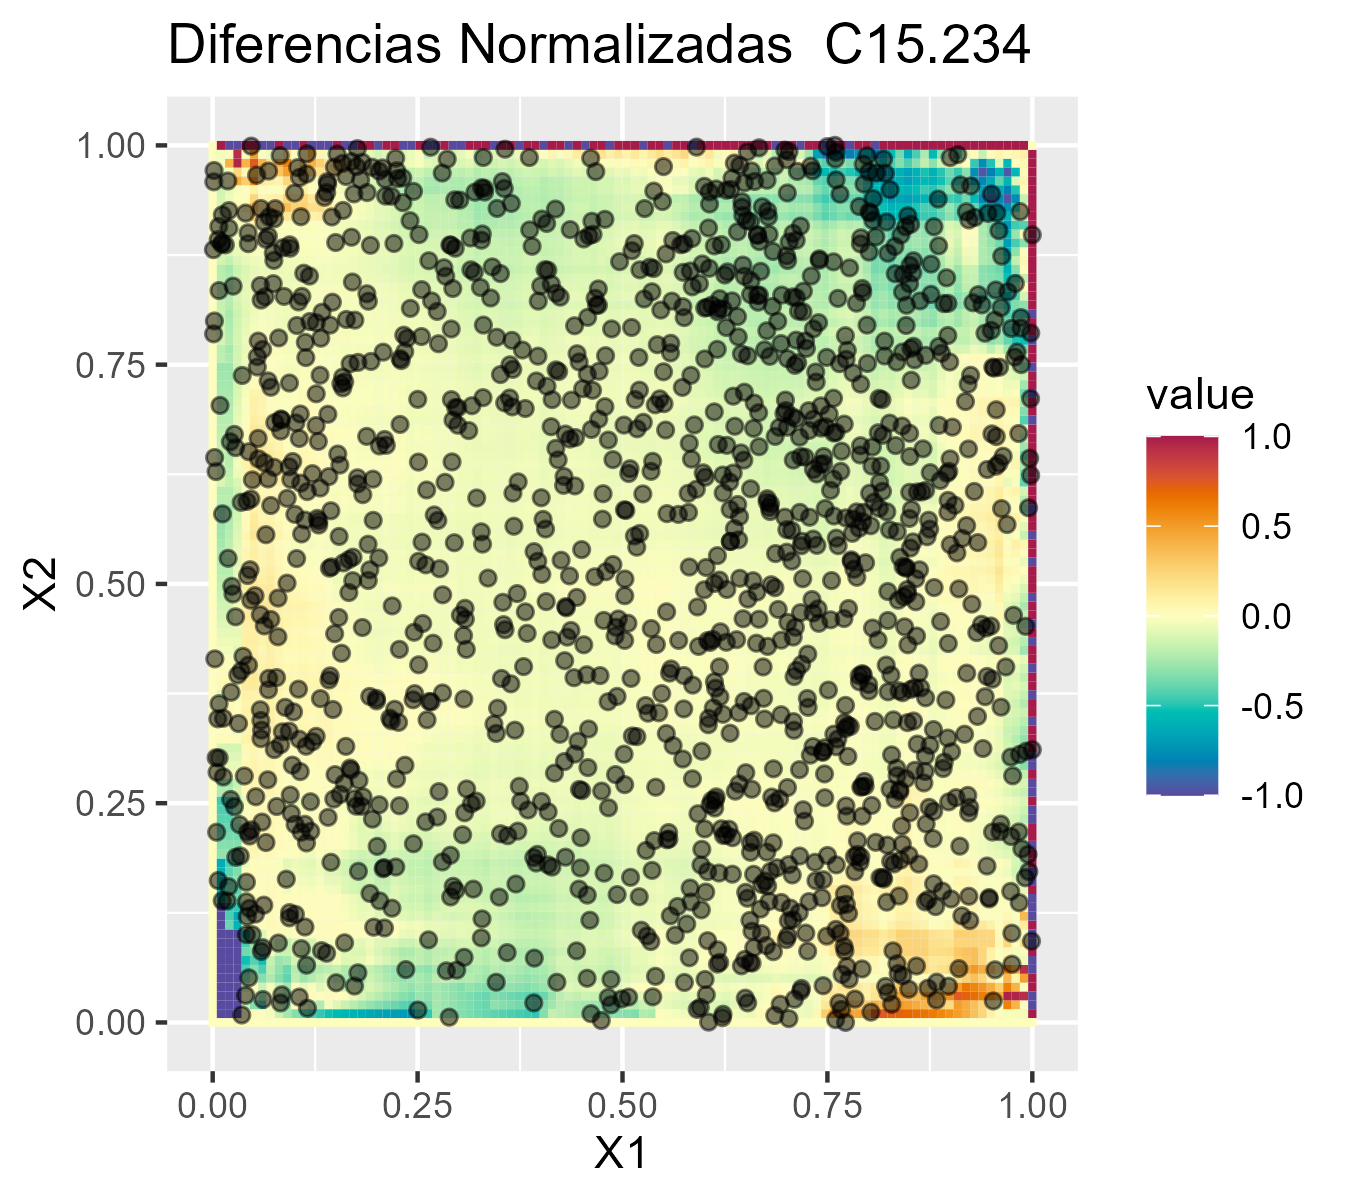
\includegraphics[width=0.3\textwidth]{4img/TotalHC15.234.png}}
    \caption{Cópulas ajustadas para mujeres y hombres, nivel $3$.}
    \label{fig:Modelo4TotalNivel4}
\end{figure}

Finalmente, en la Figura \ref{fig:Modelo4TotalNivel4} se muestra la cópula $C_{15|234}$ correspondiente al último nivel. Esta cópula representa la relación entre la variable respuesta y la presión arterial diastólica, condicionada a los niveles de glucosa en el tiempo $120$ y $0$, y el índice de masa corporal se observa una dependencia muy baja.

A continuación en la Figura \ref{fig:tabla4varTotal}, se muestra la tabla de probabilidades de tener resistencia a la insulina por clasificación de peso y glucosa para datos de hombres y mujeres. Para recordar la especificación de las clasificaciones se puede consultar las subsecciones \ref{ClasificaVar} y \ref{subTabla}.

%%%%%%%%%%%%%%%%%%%%%%%%%%%%%%%%%%%%%%%%%%%%%%%%%%%%%%%%%%%

\subsection{Tabla Resumen del Modelo}

La probabilidad de pertenecer a la clase de individuos saludables es muy alta para las personas con niveles de glucosa normales y un peso normal o con sobrepeso. En la categoría de personas con niveles de glucosa normales pero con obesidad, la probabilidad de tener resistencia a la insulina con predisfunción de las células beta aumenta. A partir de esta categoría, la probabilidad de tener resistencia a la insulina con estrés de las células beta aumenta, siendo esta la predominante en todas las clasificaciones con niveles de glucosa prediabéticos. Las categorías cuyos niveles de glucosa son diabéticos ya son clasificadas como pacientes con resistencia a la insulina con disfunción de las células beta.


\begin{figure}[H]

    \centering
    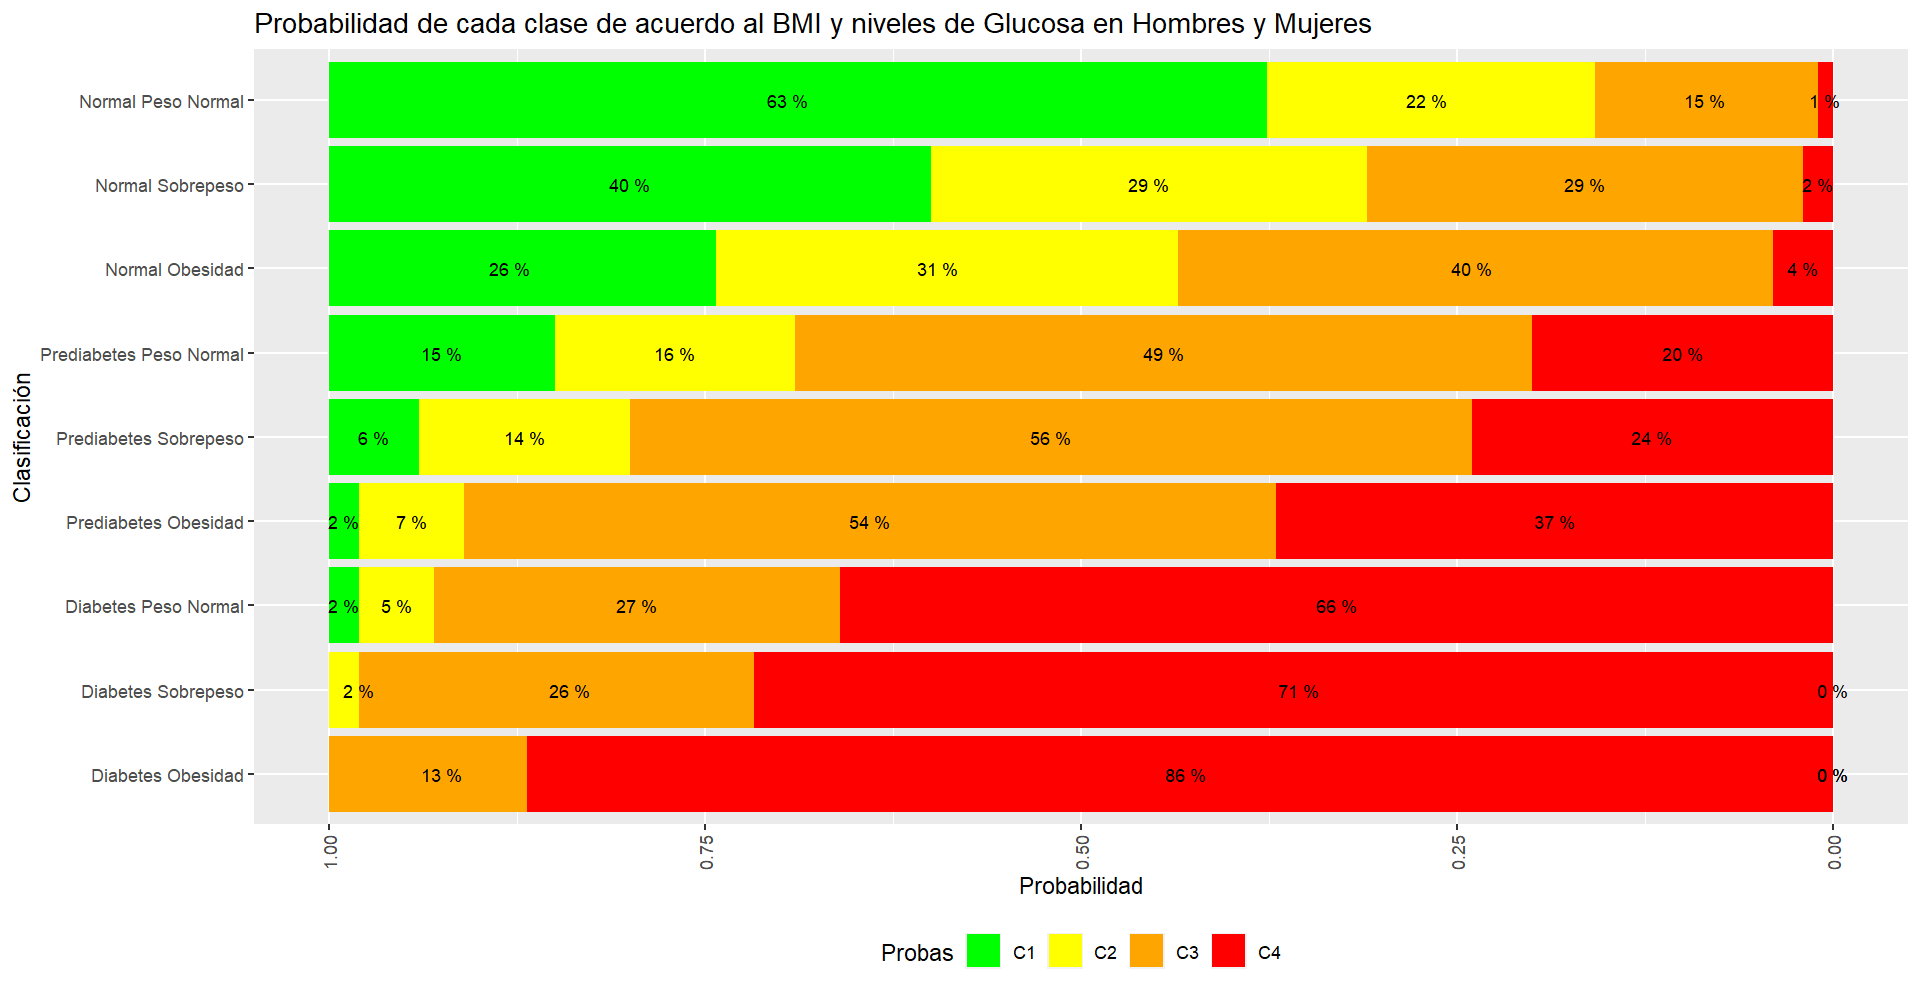
\includegraphics[height = 12 cm, width = 0.99 \textwidth]{4img/tablaT.png}
    \caption{Tabla de probabilidades de cada Clase.}
    \label{fig:tabla4varTotal}
\end{figure}



Las ventajas de tener este tipo de representaciones, y no solo quedarse con el modelo computacional, son significativas. Estas representaciones pueden llevarse a todo tipo de comunidades, incluidas aquellas con escasos recursos. Al proporcionar una visualización clara y accesible, se facilita la comprensión y el análisis de los datos sin necesidad de equipos o software avanzado. Esto es especialmente importante en áreas donde el acceso a tecnología de punta es limitado, permitiendo a los profesionales de la salud y a los encargados de la toma de decisiones identificar patrones y tomar medidas preventivas de manera más efectiva.

%%%%%%%%%%%%%%%%%%%%%%%%%%%%%%%%%%%%%%%%%%%%%%%%%%%%%%%%%
%%%%%%%  G R A F I C O S  D E  E F E C T O S  %%%%%%%%%%%
%%%%%%%%%%%%%%%%%%%%%%%%%%%%%%%%%%%%%%%%%%%%%%%%%%%%%%%%%

\subsection{Comparación de Modelos}

Con el objetivo de comparar las diferencias entre los ajustes de cada subconjunto de datos, se utilizará la gráfica de efectos para visualizar el impacto que tiene cada covariable sobre la variable respuesta. Además, se emplearán las curvas de nivel para comparar cómo son las cópulas ajustadas para cada par de variables, tanto no condicionadas como condicionadas. Estas herramientas nos permitirán evaluar de manera detallada cómo se relacionan las variables en diferentes contextos y subgrupos de datos, lo que facilitará la identificación de patrones y relaciones importantes en el modelo.

En las gráficas de efectos de la variable glucosa al tiempo $120$ se muestra en las Figuras \ref{Efec120M4}, \ref{Efec120H4} y \ref{Efec120T4}, se observa que el efecto difiere según el género. En el caso de las mujeres, esta variable influye principalmente en sus valores bajos, teniendo un efecto similar para valores mayores a $120$ $mg/dl$. Por otro lado, en los hombres, parece que la respuesta cambia poco para valores menores a aproximadamente $100$ $mg/dl$. Luego, influye significativamente en el cambio de la respuesta hasta valores menores a $300$ $mg/dl$, y vuelve a cambiar poco para valores mayores a este umbral. Estas diferencias en el efecto de la variable glucosa al tiempo $120$ entre géneros son importantes y pueden tener implicaciones significativas en el análisis y la interpretación de los resultados del modelo.

En el modelo combinado de hombres y mujeres, se observa una combinación de ambas tendencias. La gráfica muestra una tendencia descendente, similar al modelo de las mujeres, pero no tiene una forma sigmoidal tan pronunciada como la de los hombres. Sin embargo, tampoco se estanca, lo que sugiere que hay una influencia continua de la variable en la respuesta a lo largo de su rango de valores. Esta combinación de tendencias refleja la complejidad de la relación entre la variable en cuestión y la respuesta, que puede variar según el género y otros factores.

\begin{figure}[H]
 \centering
  \subfloat[Glu.120, Mujeres]{
   \label{Efec120M4}
    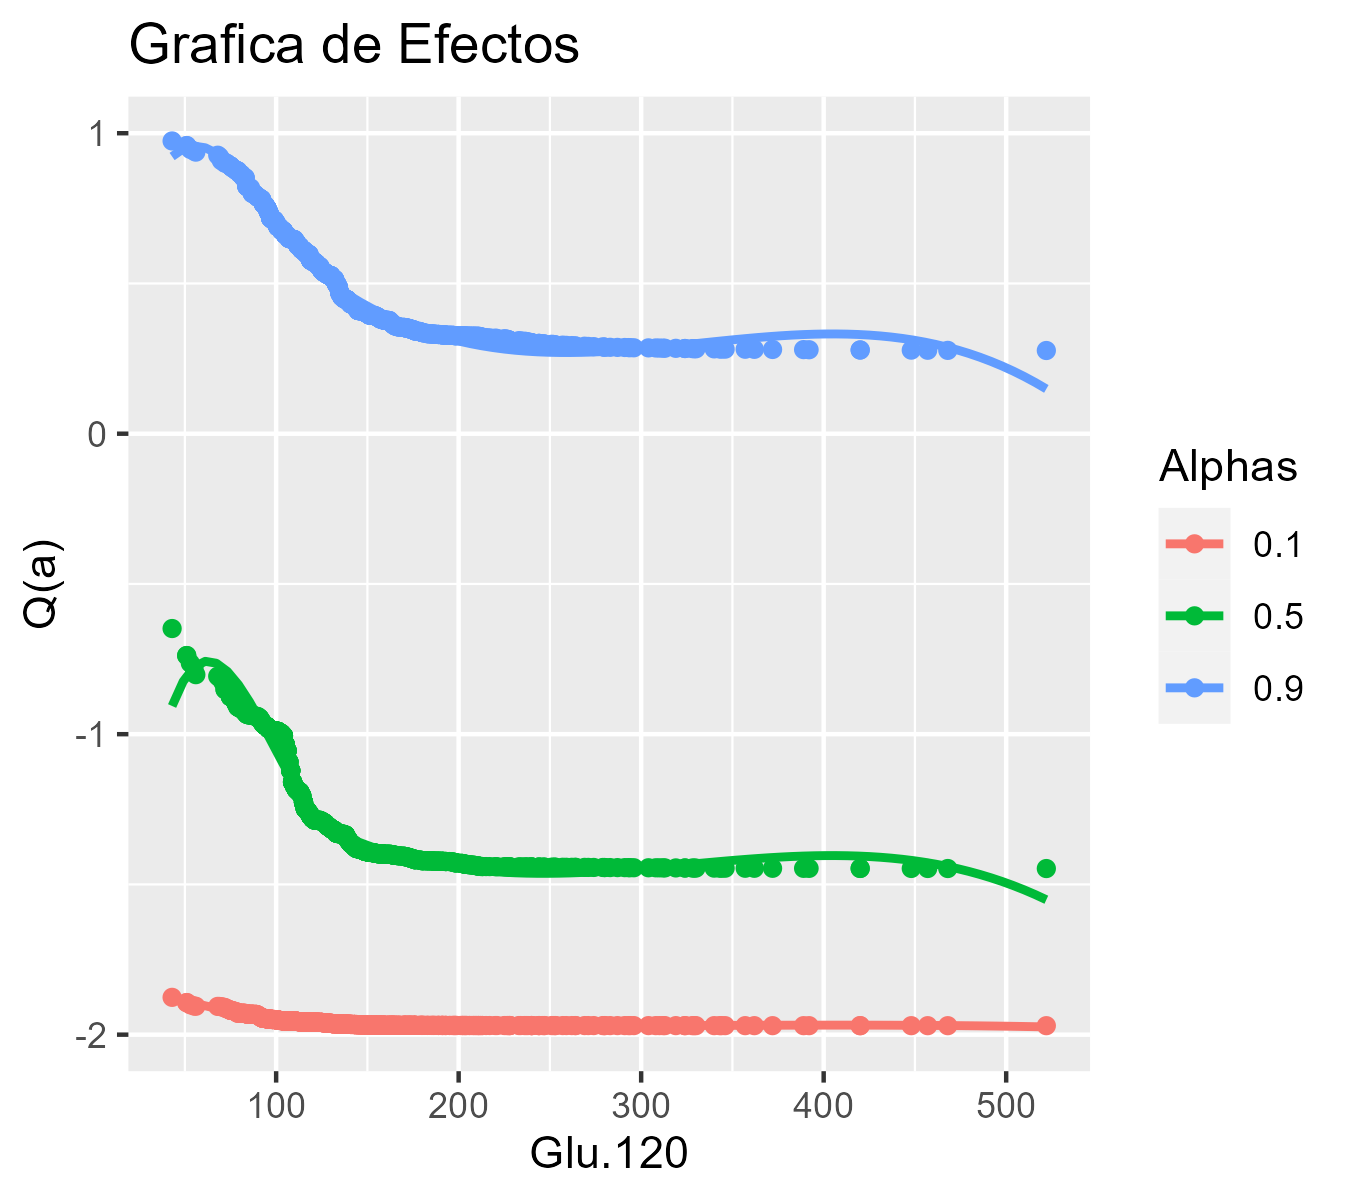
\includegraphics[width=0.3\textwidth]{4img/MujGlu.120Efec.png}}
  \subfloat[Glu.120, Hombres]{
   \label{Efec120H4}
    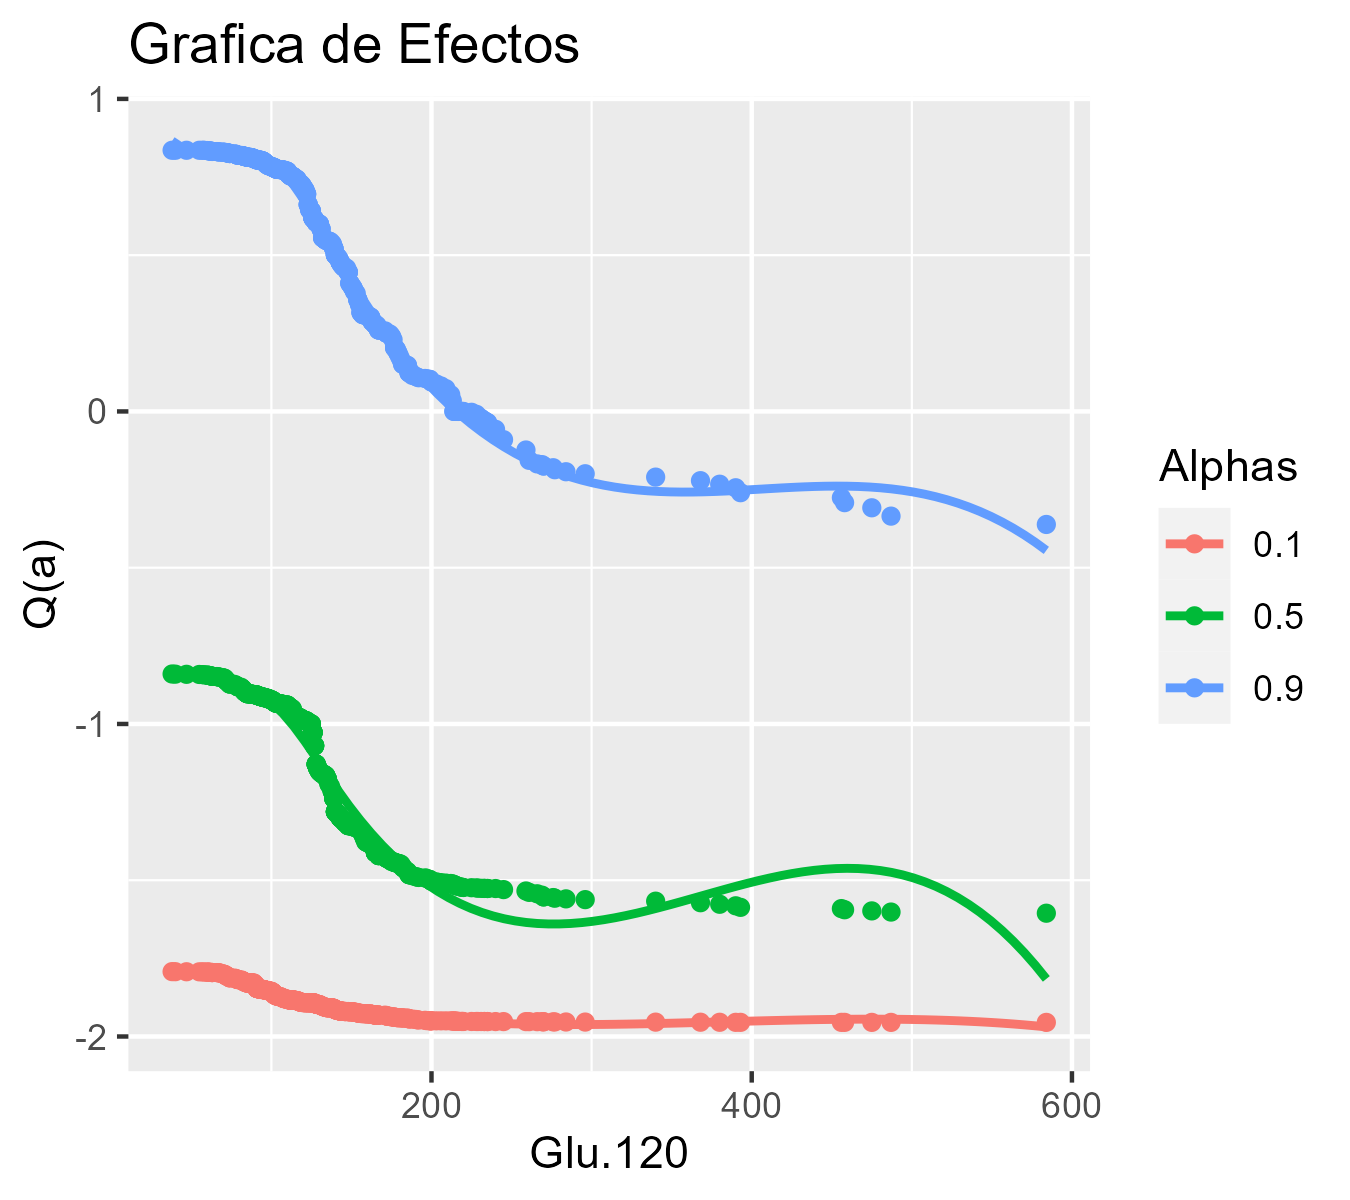
\includegraphics[width=0.3\textwidth]{4img/HomGlu.120Efec.png}}
  \subfloat[Glu.120, Total]{
   \label{Efec120T4}
    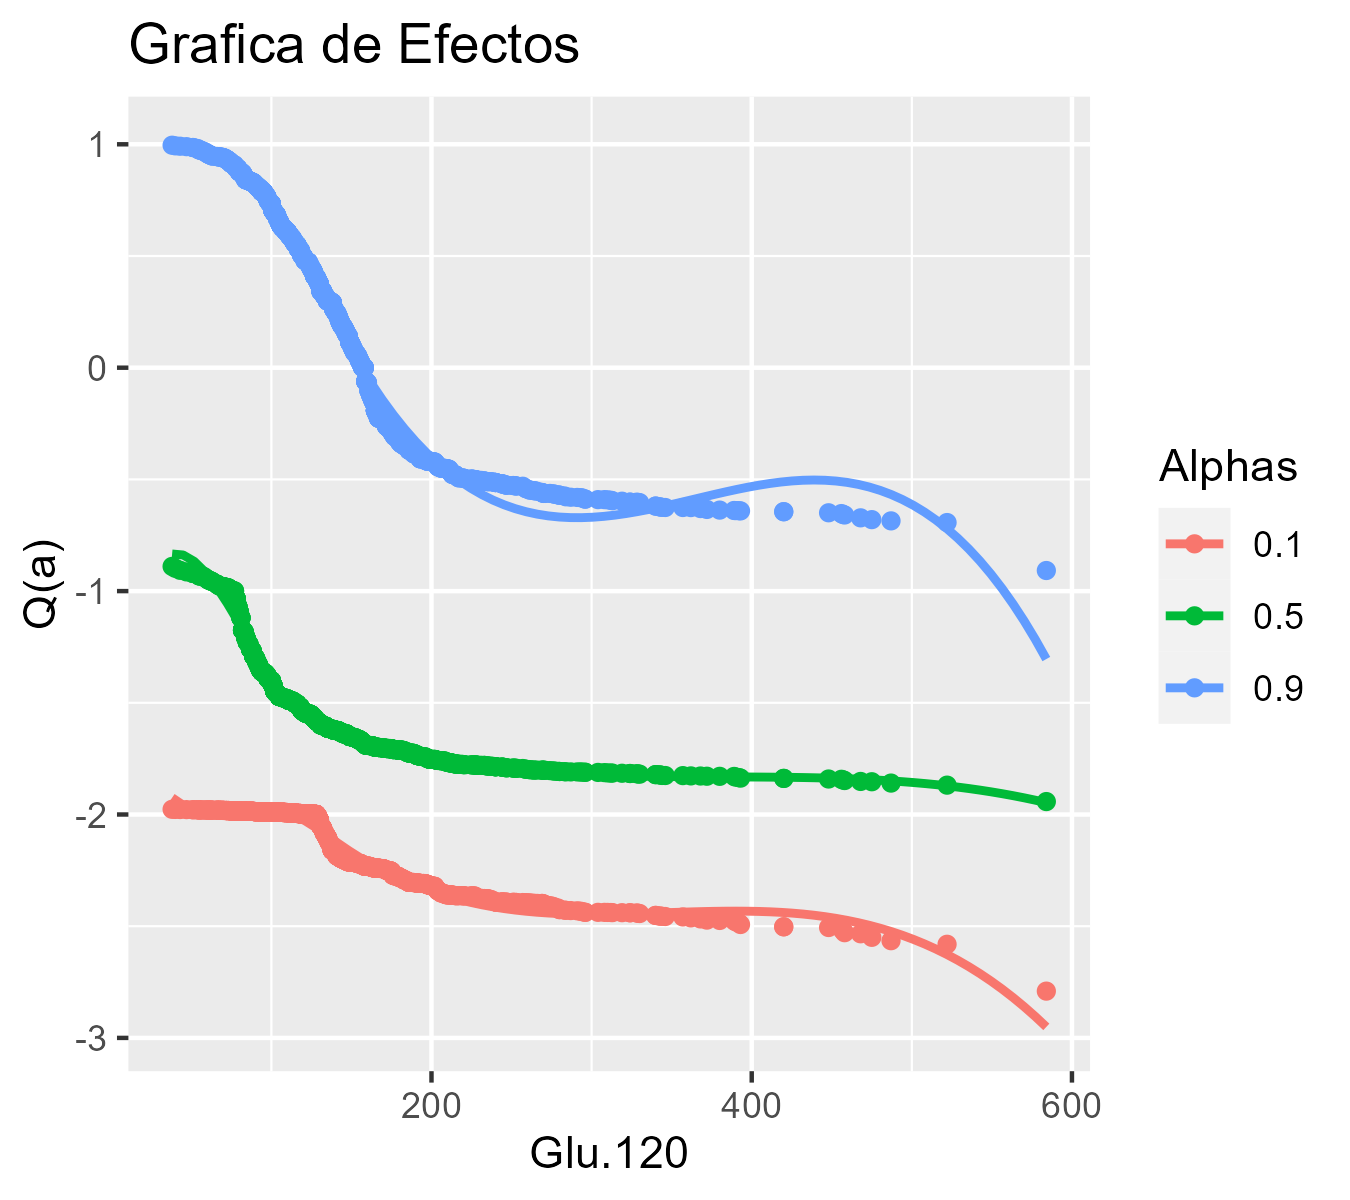
\includegraphics[width=0.3\textwidth]{4img/TotalGlu.120Efec.png}}
\end{figure}

\begin{figure}[H]
 \centering
  \subfloat[Glu.0, Mujeres]{
   \label{Efec0M4}
    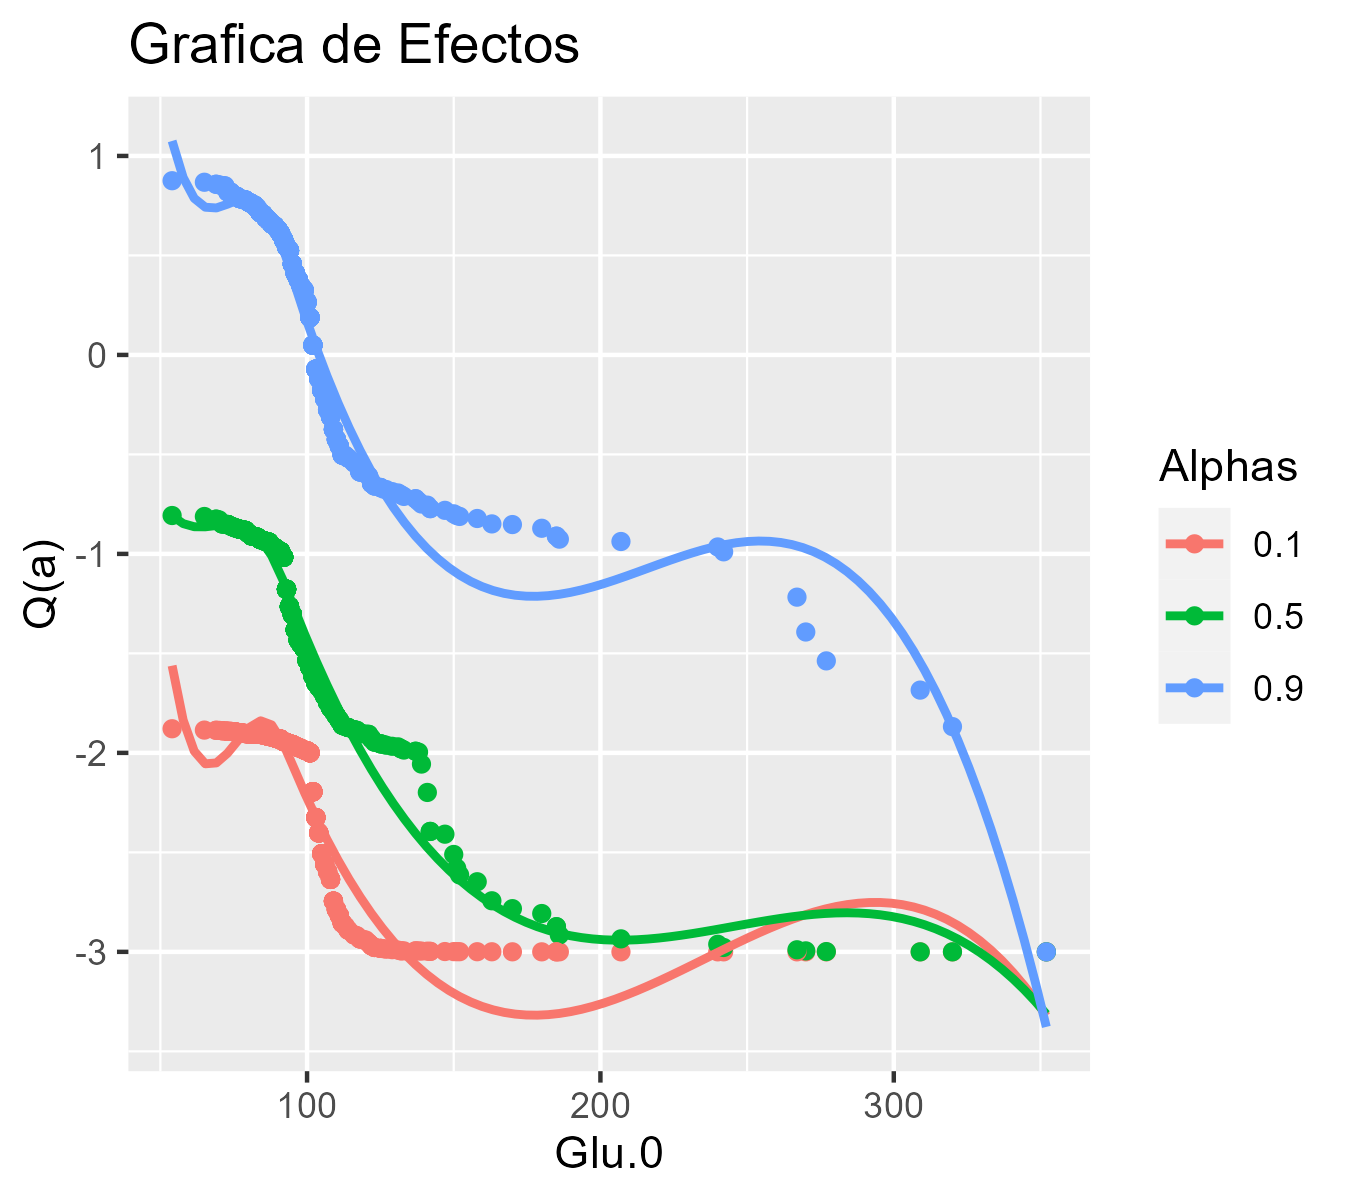
\includegraphics[width=0.3\textwidth]{4img/MujGlu.0Efec.png}}
  \subfloat[Glu.0, Hombres]{
   \label{Efec0H4}
    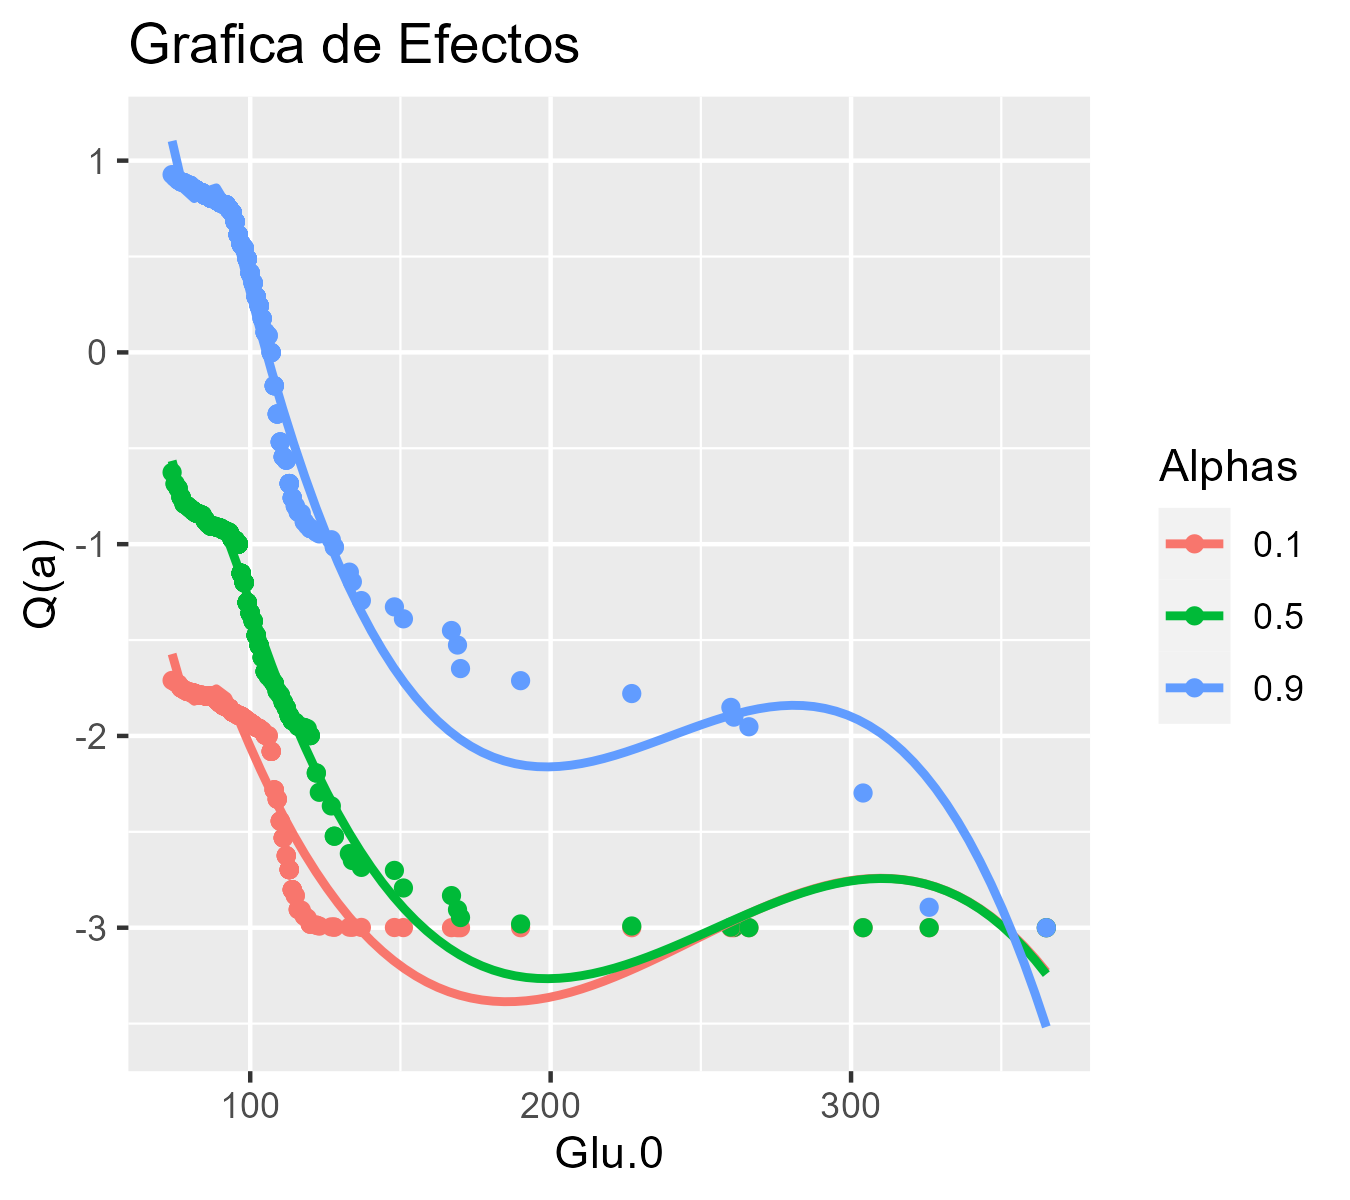
\includegraphics[width=0.3\textwidth]{4img/HomGlu.0Efec.png}}
  \subfloat[Glu.0, Total]{
   \label{Efec0T4}
    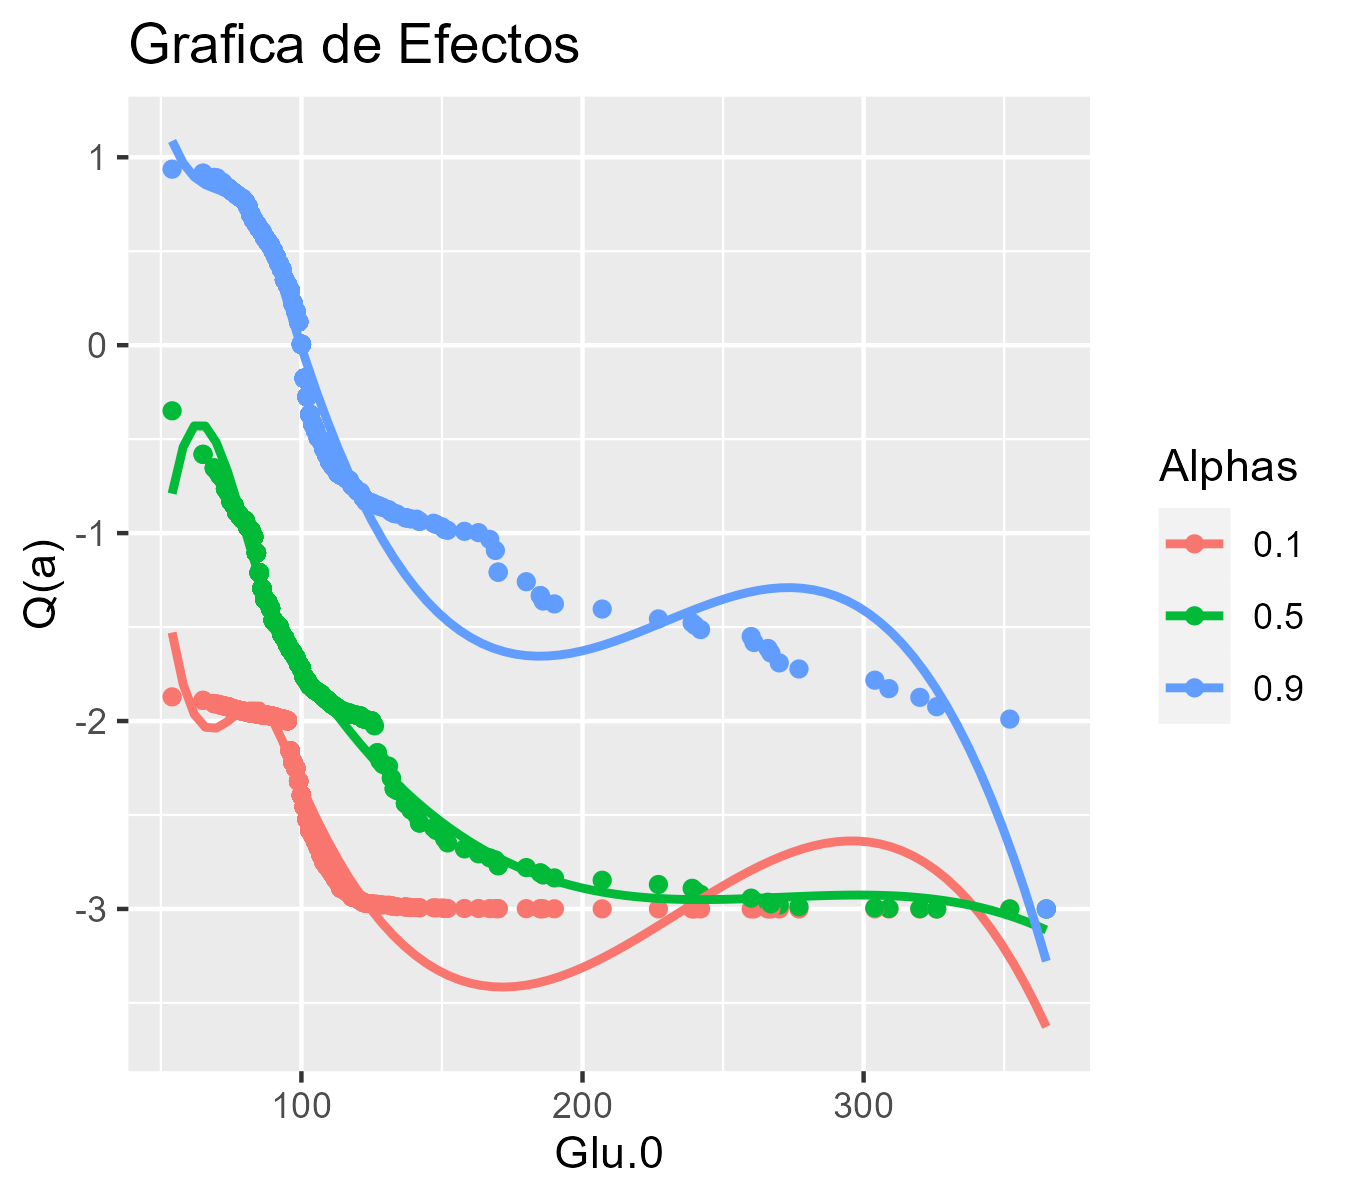
\includegraphics[width=0.3\textwidth]{4img/TotalGlu.0Efec.png}}
\end{figure}

\begin{figure}[H]
 \centering
  \subfloat[BMI, Total]{
   \label{EfecBMIM4}
    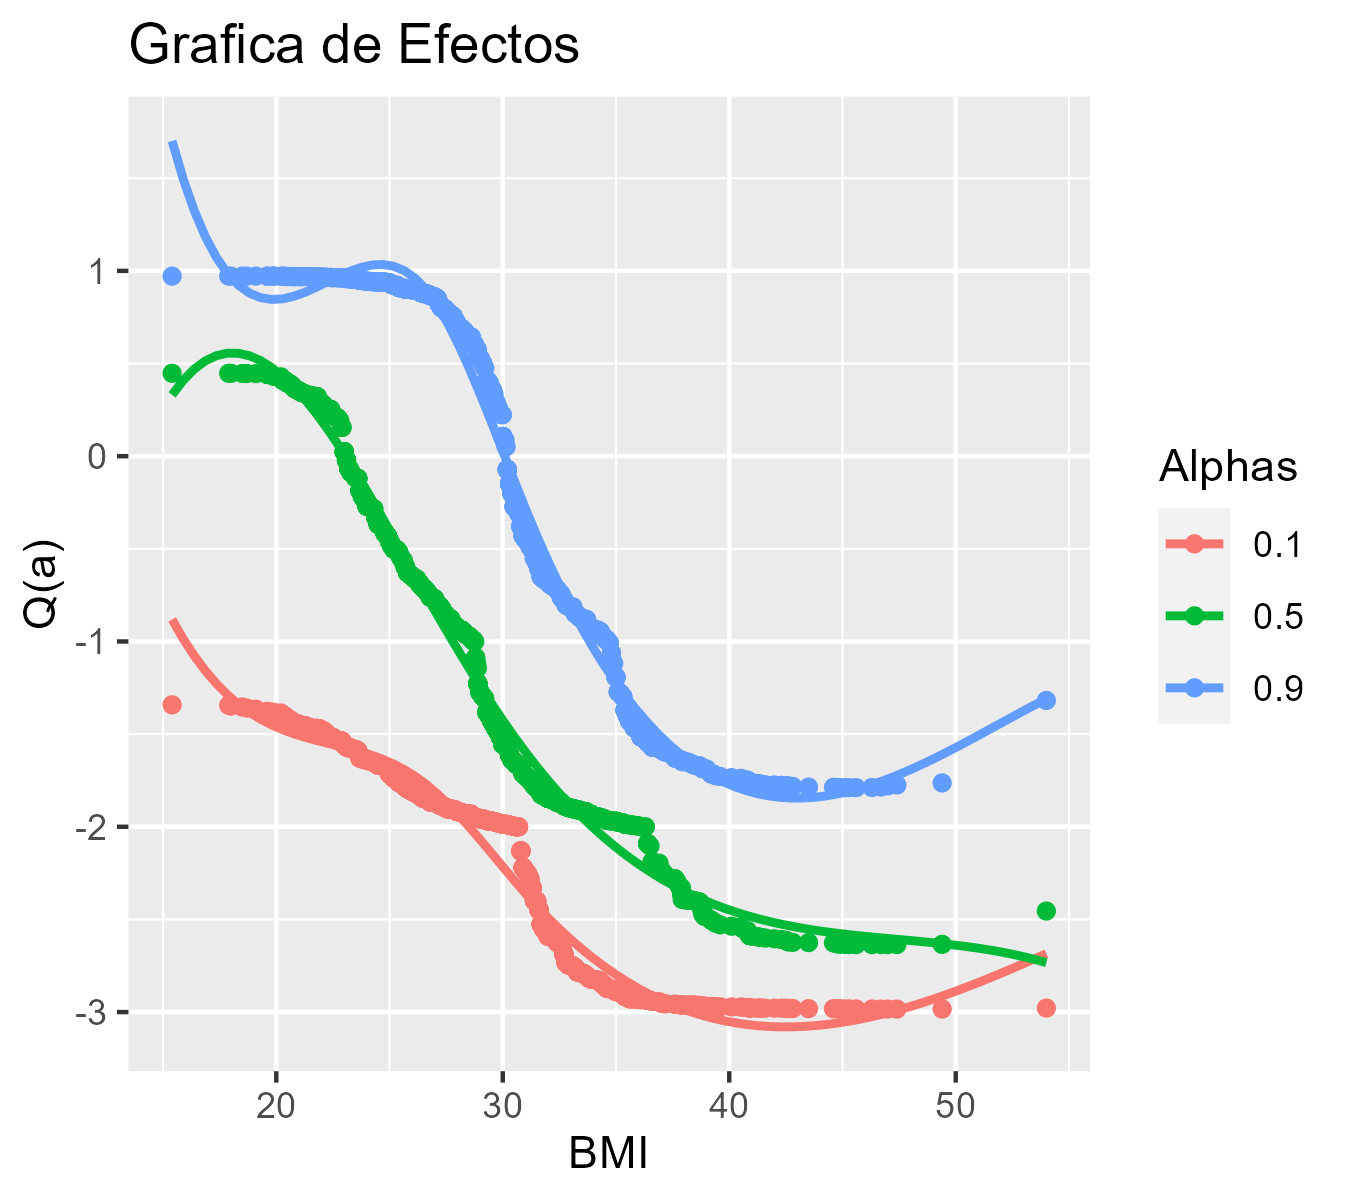
\includegraphics[width=0.3\textwidth]{4img/MujBMIEfec.png}}
  \subfloat[BMI, Total]{
   \label{EfecBMIH4}
    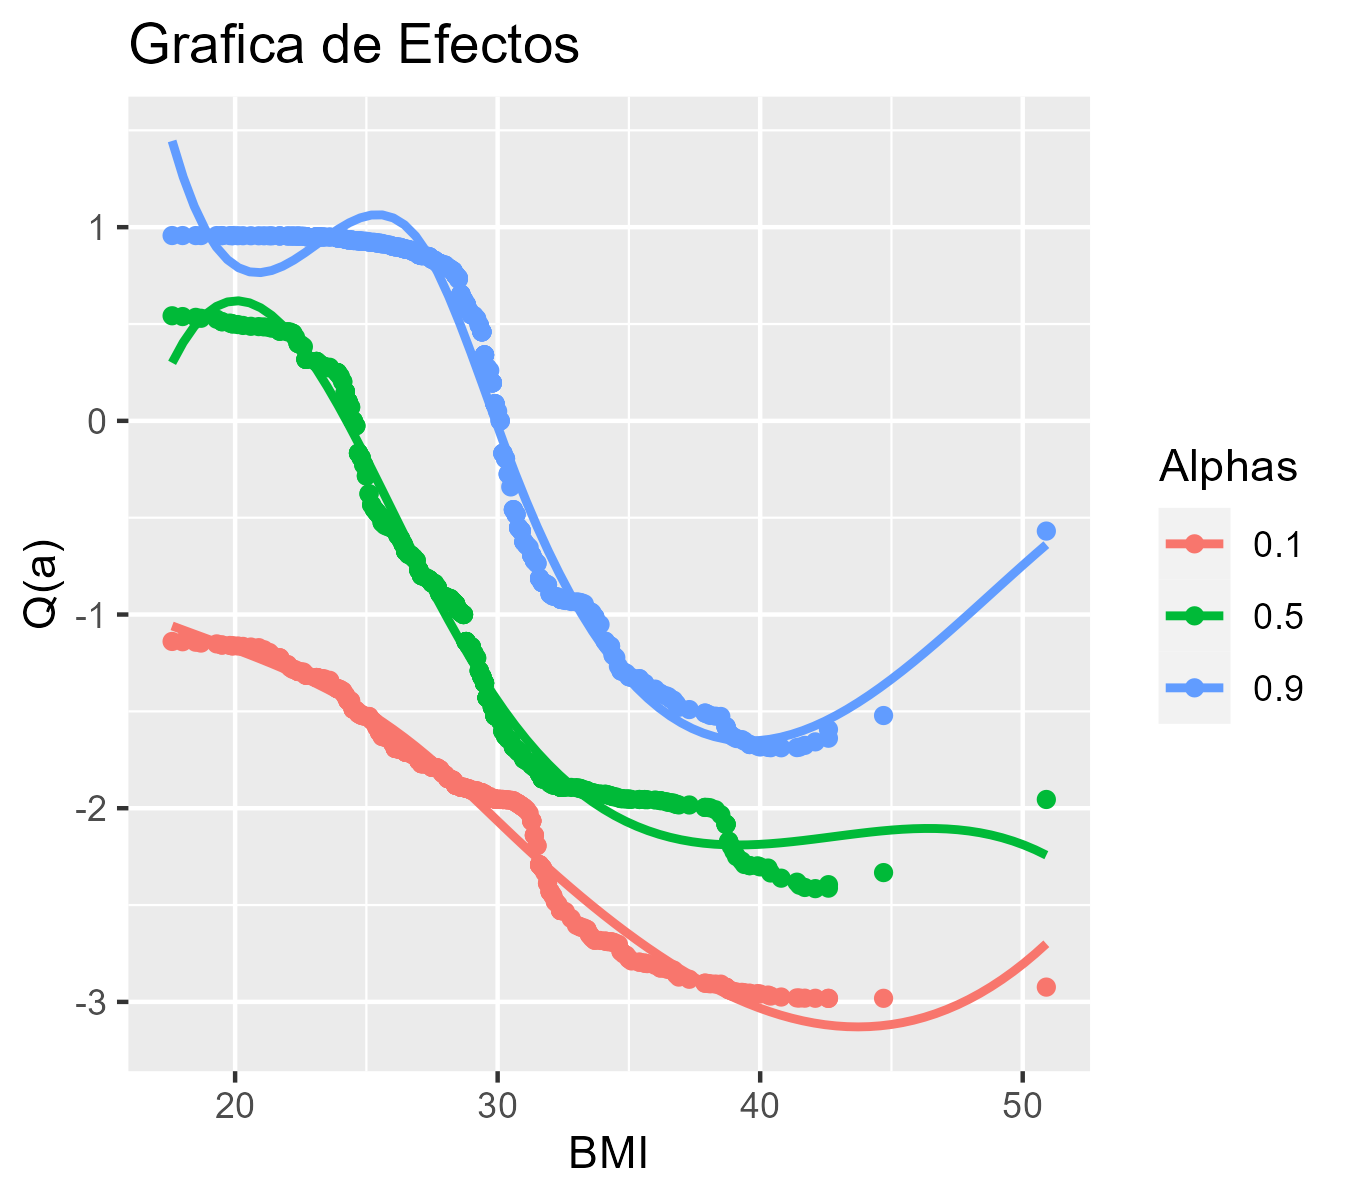
\includegraphics[width=0.3\textwidth]{4img/HomBMIEfec.png}}
  \subfloat[BMI, Total]{
   \label{EfecBMIT4}
    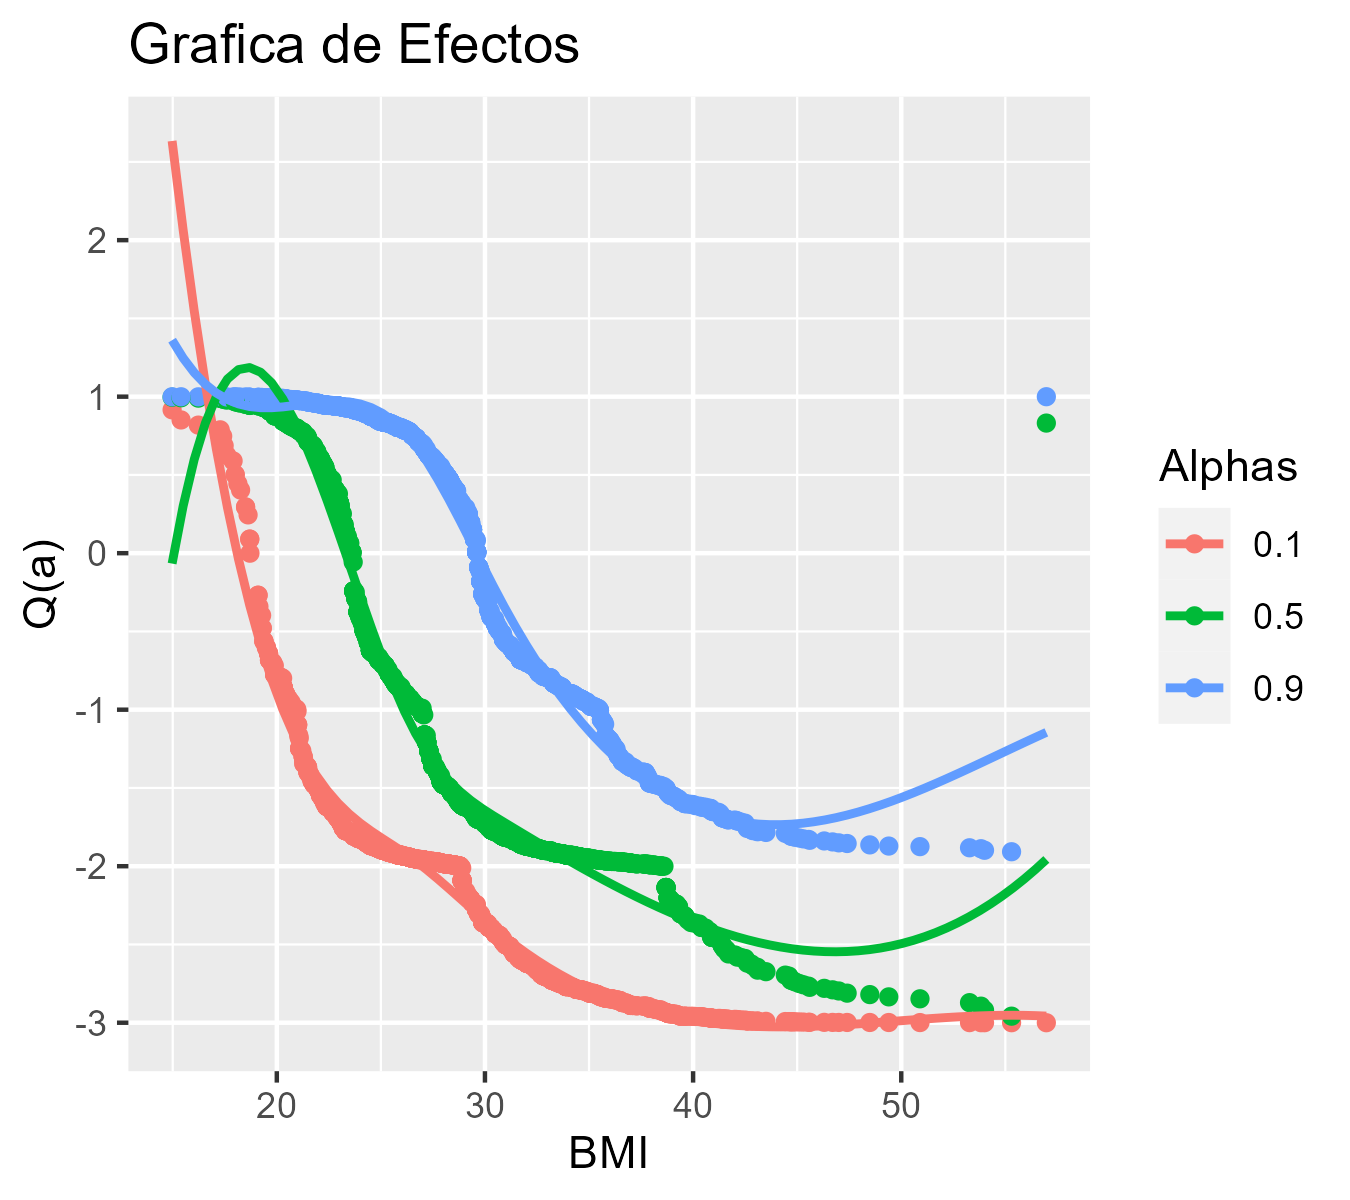
\includegraphics[width=0.3\textwidth]{4img/TotalBMIEfec.png}}
\end{figure}

\begin{figure}[H]
 \centering
  \subfloat[PA.diast, Mujeres]{
   \label{EfecPAM4}
    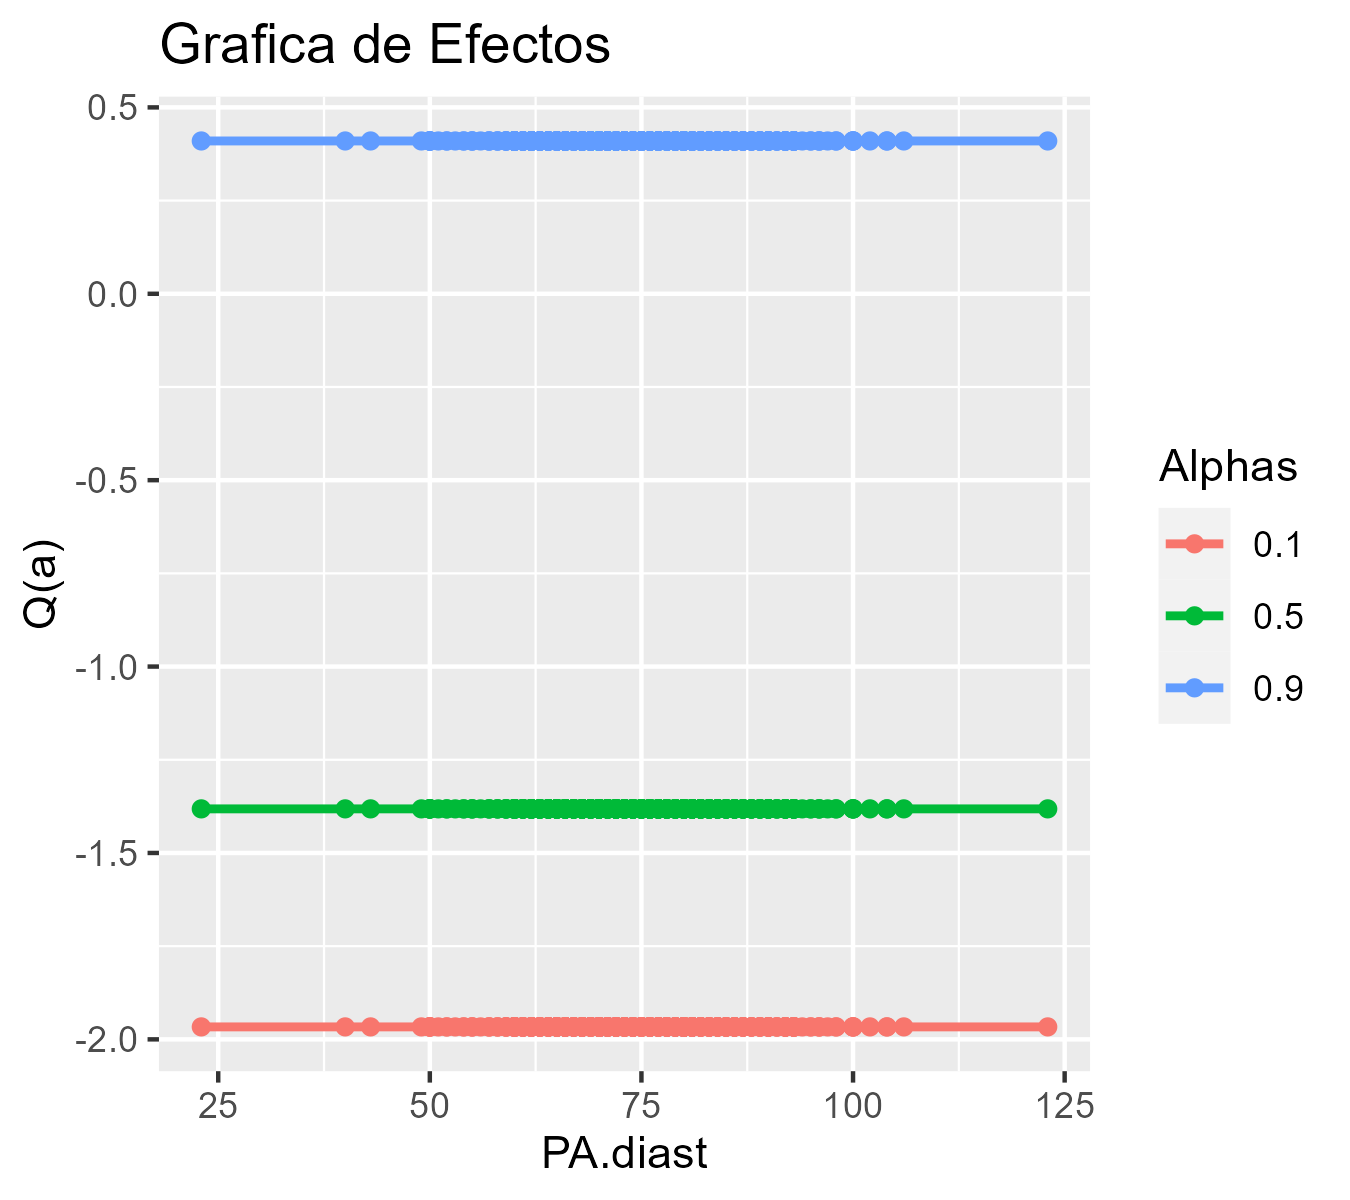
\includegraphics[width=0.3\textwidth]{4img/MujPA.diastEfec.png}}
  \subfloat[PA.diast, Hombres]{
   \label{EfecPAH4}
    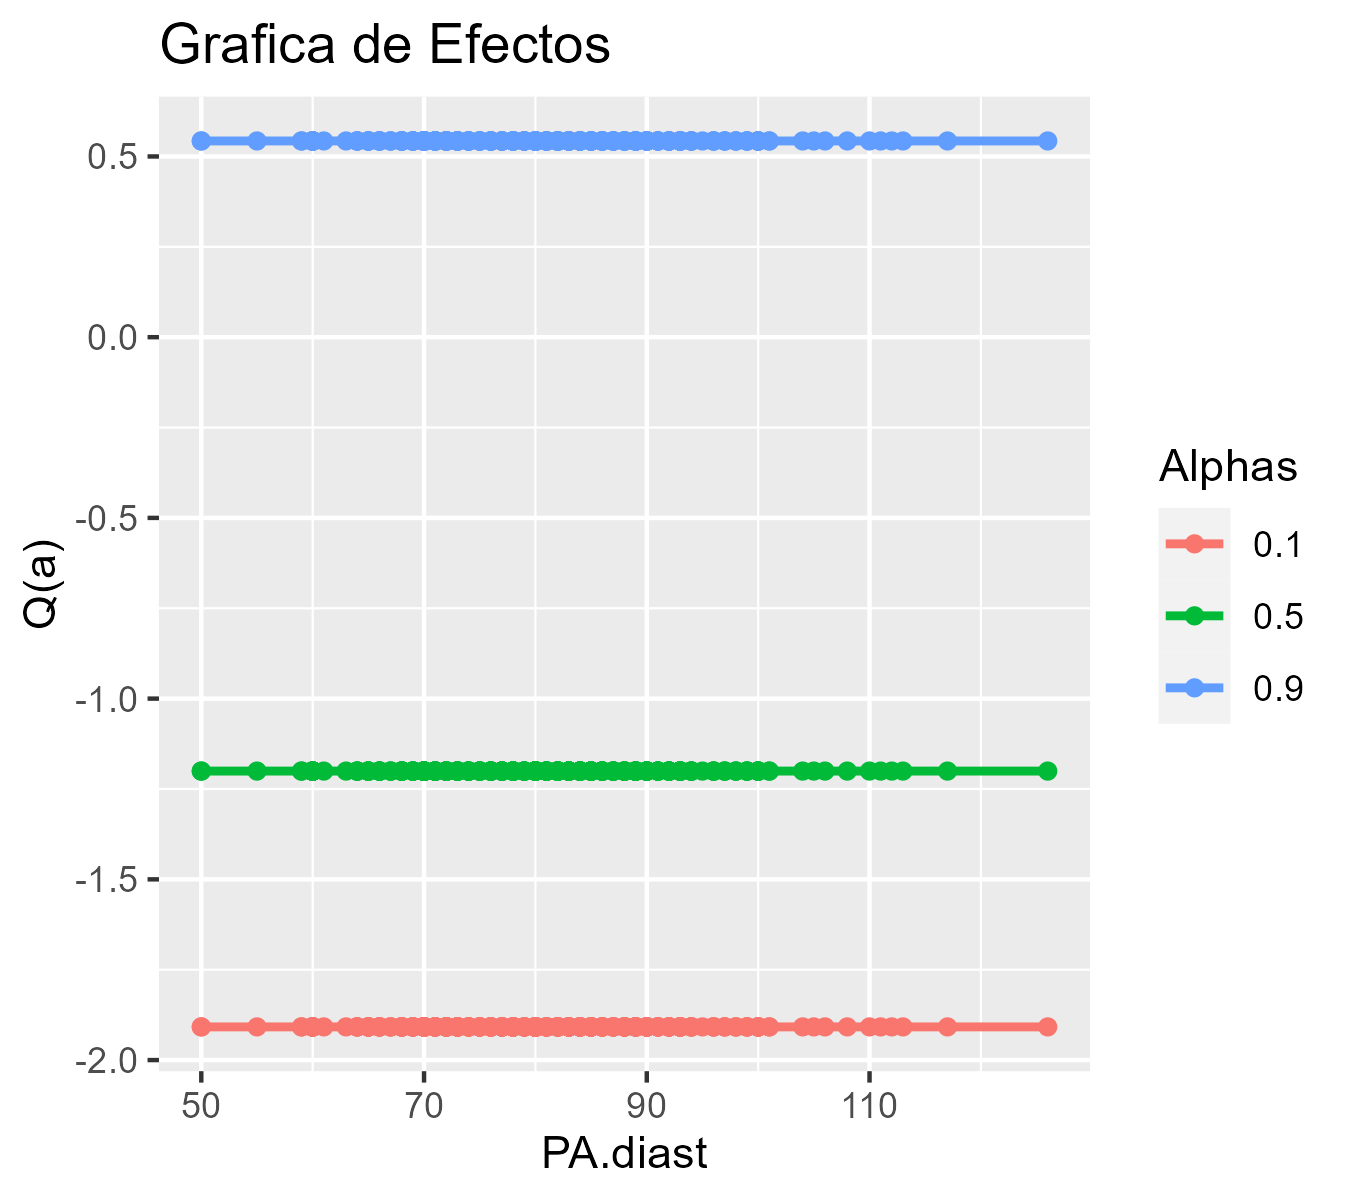
\includegraphics[width=0.3\textwidth]{4img/HomPA.diastEfec.png}}
  \subfloat[PA.diast, Total]{
   \label{EfecPAT4}
    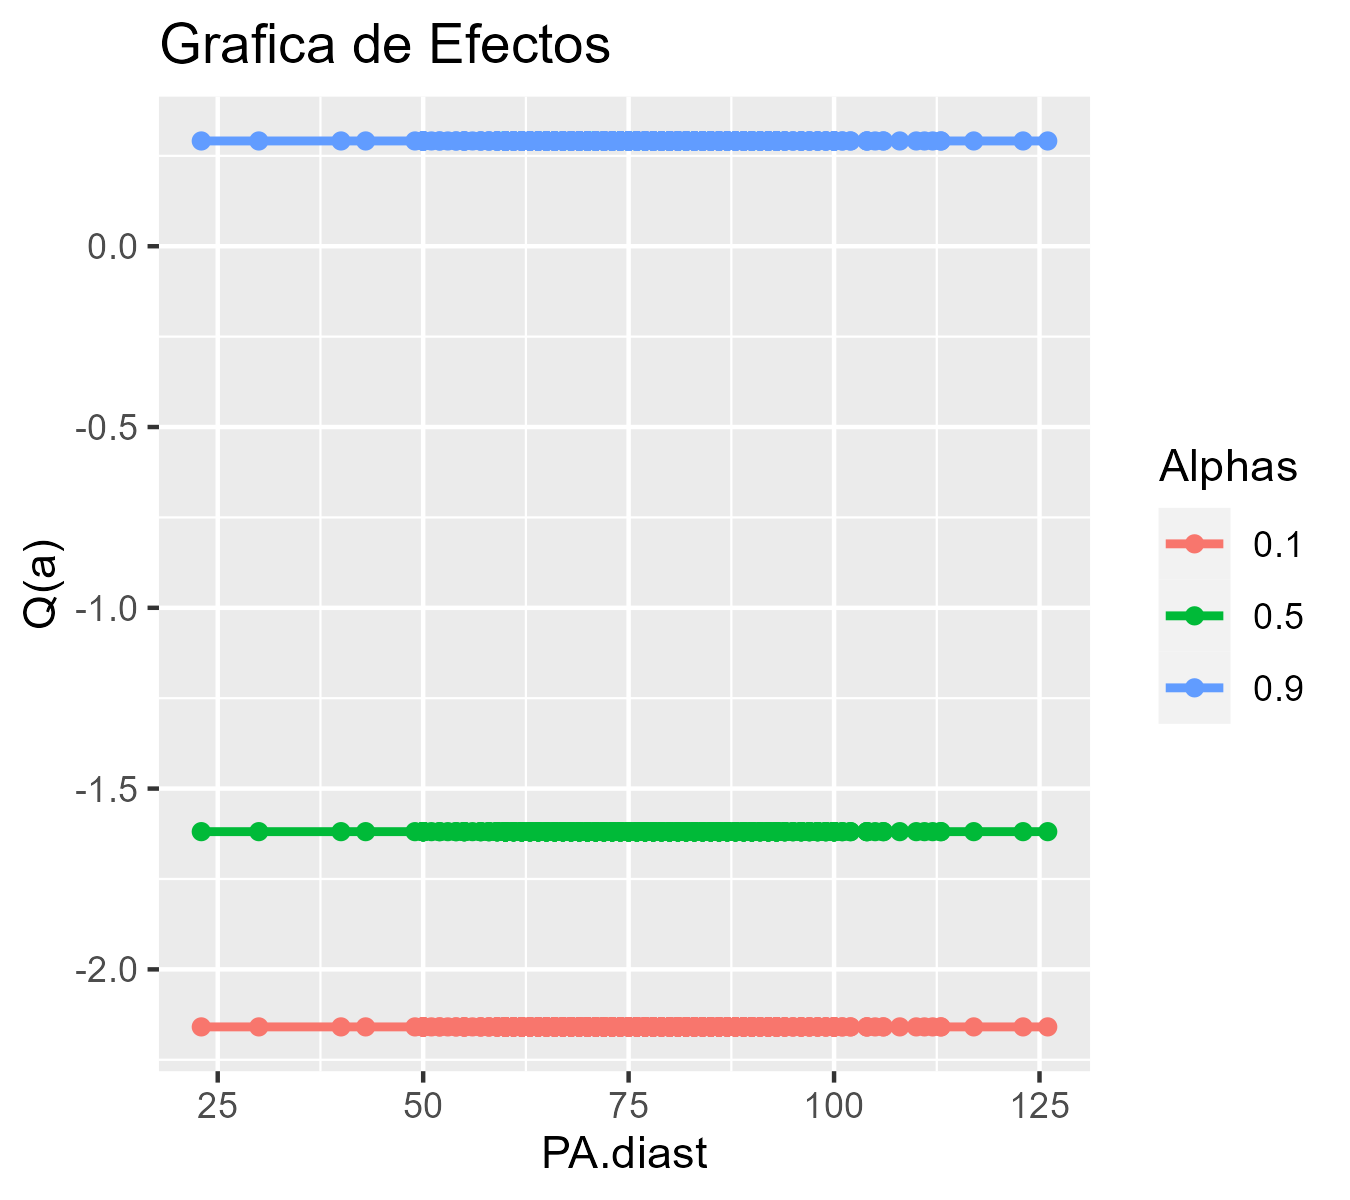
\includegraphics[width=0.3\textwidth]{4img/TotalPA.diastEfec.png}}
    \caption{Gráficas de efectos para la regresión de 4 variables.}
    \label{fig:efecto4}
\end{figure}



Ahora se analizará los efectos de la glucosa en tiempo $0$, Figuras \ref{Efec0M4}, \ref{Efec0H4} y \ref{Efec0T4} . En mujeres se observa que inicialmente influye levemente en la variable respuesta. Luego, este efecto aumenta y posteriormente disminuye. Sin embargo, el nivel de aumento o disminución depende en gran medida del cuantil que se considere. Por otro lado, en hombres, el decrecimento en la variable respuesta es muy drástico al principio, y luego se vuelve muy leve. Al igual que en mujeres, este nivel de cambio también se ve afectado por el nivel del cuantil con el que se realice la regresión. Estas diferencias en los efectos de la glucosa en tiempo $0$ entre géneros resaltan la importancia de considerar las características específicas de cada grupo al analizar los datos y desarrollar modelos predictivos.


En el efecto de la variable $Glu.0$ del modelo combinado de hombres y mujeres, parece haber un cambio en todos los valores de la glucosa, y estos cambios varían de acuerdo al nivel de la regresión. Sin embargo, es importante destacar que el rango de la variable respuesta en este modelo combinado es más grande que los rangos individuales de hombres y mujeres. Esto sugiere que la inclusión de ambos géneros puede resultar en una variabilidad más amplia en la variable respuesta, lo que podría reflejar la diversidad de respuestas dentro de la población en general. 

En las Figuras \ref{EfecPAM4}, \ref{EfecPAH4} y \ref{EfecPAT4}, se pueden observar los efectos de la variable presión diastólica sobre la variable respuesta. Se puede notar que no hay un cambio significativo en la variable respuesta ante los diferentes valores de la presión diastólica en los $3$ modelos. Esto indica que la presión diastólica no aporta información relevante al modelo, ya que su contribución es prácticamente nula en relación con la variable respuesta. Por lo tanto, se puede concluir que esta variable no tiene un impacto significativo y podría ser excluida del modelo sin perder precisión predictiva.

Los efectos de las variables $BMI$ aparecen en las Figuras \ref{EfecBMIM4}, \ref{EfecBMIH4} y \ref{EfecBMIT4}. Las interpretaciones son similares a los casos de las variables $Glu.0$ y $Glu.120$, por lo que no se describen. 

En el Apéndice \ref{ApendiceA}, se presentan las visualizaciones de los modelos D-vine ajustados específicamente para mujeres y para hombres, junto con sus respectivas tablas de probabilidades. La inclusión de estos modelos en el apéndice permite una evaluación detallada y comparativa de las diferencias y similitudes en la dependencia entre variables según el género, sin interrumpir el flujo principal del análisis en el cuerpo del documento.